\documentclass[a4paper,12pt,oneside,openright]{memoir}
\chapterstyle{veelo}

%\documentclass[draft,final]{vutinfth} % Remove option 'final' to obtain debug information.

\usepackage{TUINFDA}
\usepackage{url}
\usepackage[colorlinks=true,urlcolor=blue]{hyperref}					% links in pdf
\usepackage{graphicx}            			% Figures
\usepackage{verbatim}            			% Code-Environment
\usepackage{listings}
\usepackage{graphicx}
\usepackage{caption}
\usepackage{subfig}
\usepackage{float}
\usepackage{amsmath}


% hglanzer: problem workstation@labor <--> laptop
%\usepackage[lined,linesnumbered,algochapter]{algorithm2e} % Algorithm-Environment
\usepackage[lined,linesnumbered,algochapter,norelsize]{algorithm2e} % Algorithm-Environment


\usepackage{pgf}					
\usepackage{tikz}					% tikz graphics
\usetikzlibrary{arrows,automata}
\usepackage[toc]{glossaries}

\makeglossary
\loadglsentries{acronyms}

\usepackage[backend=bibtex, sorting=none]{biblatex}
\addbibresource{references.bib}

%%%%%%%%%%%%%%%%%%%%%%%%%%%%%%%%%%%%%%%%%%%%%%%%%%%%%%%%%%%%%%%%%%%%%%%%%%%%%%%%%

\thesistitle{Highly available KNX networks}
%\thesissubtitle{Building a secure and dependable Layer} % optional
\thesisdate{14.8.2015}

% all titles and designations have to be gender-related!
\thesisdegree{Diplom-Ingenieur}{Diplom-Ingenieur}
\thesiscurriculum{Technische Informatik}{Computer Engineering} % your study
\thesisverfassung{Verfasser} % Verfasser
\thesisauthor{B.Sc. Harald Glanzer} % your name
\thesisauthoraddress{Hardtgasse 25 / 12A, 1190 Wien} % your address
\thesismatrikelno{0727156} % your registration number

\thesisbetreins{Ao.Univ-Prof. DI Dr. Wolfgang Kastner}
\thesisbetrzwei{DI Dr. Lukas Krammer}
%\thesisbetrdrei{Dr. Vorname Familienname} % optional

% define page numbering styles
\makepagestyle{numberCorner}
\makeevenfoot{numberCorner}{\thepage}{}{}
\makeoddfoot{numberCorner}{}{}{\thepage}

% define custom macros for specific formats or names
\newcommand{\uml}[1]{\texttt{#1}}
\newcommand{\cd}{\textsf{Class Diagram}}

% for shell command snippets
\newcommand{\shellcmd}[1]{\\\indent\indent\texttt{\footnotesize\# #1}\\}

% for shell command snippets with multiple lines
\lstdefinestyle{BashInputStyle}{
  language=bash,
  basicstyle=\small\sffamily,
  numbers=left,
  numberstyle=\tiny,
  numbersep=3pt,
  %frame=tb,
  columns=fullflexible,
  backgroundcolor=\color{yellow!20},
  linewidth=0.9\linewidth,
  xleftmargin=0.1\linewidth,
  breaklines=true,
  showstringspaces=false,
  captionpos=b
}

\lstdefinestyle{Cstyle}{
  language=C,
  basicstyle=\small\sffamily,
  numbers=left,
  numberstyle=\tiny,
  numbersep=3pt,
  %frame=tp,			% top bottom frame
  columns=fullflexible,
  backgroundcolor=\color{yellow!20},
  linewidth=0.95\linewidth,
  xleftmargin=0.1\linewidth,
  breaklines=true,
  keepspaces=true,
  captionpos=b,
  showstringspaces=false
}

\begin{document}

\captionnamefont{\bfseries}

%%%%%%%%%%%%%%%%%%%%%%%%%%%%%%%%%%%%%%%%%
%%%   FRONTMATTER    %%%%%%%%%%%%%%%%%%%%
%%%%%%%%%%%%%%%%%%%%%%%%%%%%%%%%%%%%%%%%%
\frontmatter
\pagenumbering{roman}

%%%%%%%%%%%%%%%%%%%%%%%%%%%%%%%%%%%%%%%%%
%%%   TITLEPAGES    %%%%%%%%%%%%%%%%%%%%%
%%%%%%%%%%%%%%%%%%%%%%%%%%%%%%%%%%%%%%%%%

% the german title page is required as first page
% $Id: titlepage.tex 1752 2010-03-20 11:07:02Z tkren $
%
% TU Wien - Faculty of Informatics
% thesis titlepage
%
% This titlepage is using the geometry package, see
% <http://www.ctan.org/macros/latex/contrib/geometry/geometry.pdf>
%
% For questions and comments send an email to
% Thomas Krennwallner <tkren@kr.tuwien.ac.at>
% or to Petra Brosch <brosch@big.tuwien.ac.at>
%

\selectlanguage{ngerman}

% setup page dimensions for titlepage
\newgeometry{left=2.4cm,right=2.4cm,bottom=2.5cm,top=2cm}

% force baselineskip and parindent
\newlength{\tmpbaselineskip}
\setlength{\tmpbaselineskip}{\baselineskip}
\setlength{\baselineskip}{13.6pt}
\newlength{\tmpparindent}
\setlength{\tmpparindent}{\parindent}
\setlength{\parindent}{17pt}

% first titlepage
\thispagestyle{tuinftitlepage}

%
% Kludge: for each titlepage set \pagenumbering to a different
% style. This is used to fix a problem with hyperref, because there
% are multiple "page 1" and hyperref hates that
%
\pagenumbering{Alph}

\begin{center}
{\ \vspace{3.4cm}}

\begin{minipage}[t][2.8cm][s]{\textwidth}%
\centering
\thesistitlefontHUGE\sffamily\bfseries\tuinfthesistitle\\
\bigskip
{\thesistitlefonthuge\sffamily\bfseries\tuinfthesissubtitle}
\end{minipage}

\vspace{1.3cm}

{\thesistitlefontLARGE\sffamily \tuinfthesistype}

\vspace{6mm}

{\thesistitlefontlarge\sffamily zur Erlangung des akademischen Grades}

\vspace{6mm}

{\thesistitlefontLARGE\sffamily\bfseries \tuinfthesisdegree}

\vspace{6mm}

{\thesistitlefontlarge\sffamily im Rahmen des Studiums}

\vspace{6mm}

{\thesistitlefontLarge\sffamily\bfseries \tuinfthesiscurriculum}

\vspace{6.5mm}

{\thesistitlefontlarge\sffamily eingereicht von}

\vspace{6mm}

{\thesistitlefontLarge\sffamily\bfseries \tuinfthesisauthor}

\vspace{1.5mm}

{\thesistitlefontlarge\sffamily Matrikelnummer \tuinfthesismatrikelno} 

\vspace{1.4cm}

\vspace{0pt}\raggedright\thesistitlefontnormalsize\sffamily
\begin{minipage}[t][1.6cm][t]{\textwidth}%
  %
  an der

  Fakult\"{a}t f\"{u}r Informatik der Technischen Universit\"{a}t Wien
\end{minipage}

\begin{minipage}[t][4cm][t]{\textwidth}%
  \vspace{0pt}\raggedright\thesistitlefontnormalsize\sffamily
  %
  \begin{tabbing}%
	    \hspace{19mm} \= \hspace{66mm} \kill
	    \tuinfthesisbetreuung: \> \tuinfthesisbetreins\\
	    Mitwirkung: \> \tuinfthesisbetrzwei\\
	                \> \tuinfthesisbetrdrei
  \end{tabbing}
\end{minipage}

\begin{minipage}[t][1.5cm][t]{\textwidth}%
  \vspace{0pt}\sffamily\thesistitlefontnormalsize
  \begin{tabbing}%
    \hspace{45mm} \= \hspace{63mm} \= \hspace{51mm} \kill
    Wien, \tuinfthesisdate \> {\raggedright\rule{51mm}{0.5pt}} \> {\raggedright\rule{51mm}{0.5pt}} \\
    \> \begin{minipage}[t][0.5cm][t]{51mm}\centering (Unterschrift \tuinfthesisverfassung)\end{minipage}
    \> \begin{minipage}[t][0.5cm][t]{51mm}\centering (Unterschrift \tuinfthesisbetreuung)\end{minipage}
    \end{tabbing}
\end{minipage}

\end{center}

% we want an empty page right after first titlepage
\pagestyle{empty}
\cleardoublepage

% we're done with the titlepages, proceed with default pagenumbering
\pagenumbering{roman}

% restore baselineskip
\setlength{\baselineskip}{\tmpbaselineskip}
\setlength{\parindent}{\tmpparindent}

% back to normal geometry
\restoregeometry

\selectlanguage{english}

%%% Local Variables:
%%% TeX-PDF-mode: t
%%% TeX-debug-bad-boxes: t
%%% TeX-parse-self: t
%%% TeX-auto-save: t
%%% reftex-plug-into-AUCTeX: t
%%% End:


% an english translation may follow
% $Id: titlepage.tex 1752 2010-03-20 11:07:02Z tkren $
%
% TU Wien - Faculty of Informatics
% thesis titlepage
%
% This titlepage is using the geometry package, see
% <http://www.ctan.org/macros/latex/contrib/geometry/geometry.pdf>
%
% For questions and comments send an email to
% Thomas Krennwallner <tkren@kr.tuwien.ac.at>
% or to Petra Brosch <brosch@big.tuwien.ac.at>
%

\selectlanguage{english}

% setup page dimensions for titlepage
\newgeometry{left=2.4cm,right=2.4cm,bottom=2.5cm,top=2cm}

% force baselineskip and parindent
%\newlength{\tmpbaselineskip}
%\setlength{\tmpbaselineskip}{\baselineskip}
%\setlength{\baselineskip}{13.6pt}
%\newlength{\tmpparindent}
%\setlength{\tmpparindent}{\parindent}
%\setlength{\parindent}{17pt}

% first titlepage
\thispagestyle{tuinftitlepage}

\pagenumbering{Roman}

\begin{center}
{\ \vspace{5cm}}

\begin{minipage}[t][2.8cm][s]{\textwidth}%
\centering
\thesistitlefonthuge\sffamily\bfseries\tuinfthesistitle\\
\bigskip
\bigskip
\bigskip
\bigskip
{\thesistitlefontHUGE\sffamily\bfseries\tuinfthesissubtitle\HUGE}
\\
~
\\
%Building a Security Gateway for KNX networks with improved availability
\end{minipage}

{\ \vspace{6cm}}

\vspace{0pt}\raggedright\sffamily\Large
\begin{minipage}[t][4cm][t]{\textwidth}%
  \begin{tabbing}%
	     \hspace{40mm} \= \hspace{66mm} \kill
	    Author:\> B.Sc. Harald Glanzer\\  
	    \hspace{40mm} \= \hspace{66mm} \kill
	    Advisor:\> \tuinfthesisbetreins\\
	    Assistance: \> \tuinfthesisbetrzwei\\
	    \\
	    Department:\>  Institute of Computer Aided Automation\\
	    \>Automation Systems Group
     \end{tabbing}
\end{minipage}

{\ \vspace{4cm}}


\begin{minipage}[t][1.5cm][t]{\textwidth}%
  \vspace{0pt}\sffamily\thesistitlefontnormalsize
  \begin{tabbing}%
    \hspace{45mm} \= \hspace{63mm} \= \hspace{51mm} \kill
    Vienna, \tuinfthesisdate \> {\raggedright\rule{51mm}{0.5pt}} \> {\raggedright\rule{51mm}{0.5pt}} \\
    \> \begin{minipage}[t][0.5cm][t]{51mm}\centering (Signature of Author)\end{minipage}
    \> \begin{minipage}[t][0.5cm][t]{51mm}\centering (Signature of Advisor)\end{minipage}
    \end{tabbing}
\end{minipage}

\end{center} % optional

%%%%%%%%%%%%%%%%%%%%%%%%%%%%%%%%%%%%%%%%%
%%%   ERKLAERUNG DER SELBSTAENDIGKEIT   %
%%%%%%%%%%%%%%%%%%%%%%%%%%%%%%%%%%%%%%%%%
\cleardoublepage
\selectlanguage{ngerman}
\chapter*{Erklärung zur Verfassung der Arbeit}

\tuinfthesisauthor\\
\tuinfthesisauthoraddress

\vspace*{1.2cm}

Hiermit erkläre ich, dass ich diese Arbeit selbständig verfasst habe, 
dass ich die verwendeten Quellen und Hilfsmittel vollständig angegeben 
habe und dass ich die Stellen der Arbeit - einschließlich Tabellen, 
Karten und Abbildungen -, die anderen Werken oder dem Internet im 
Wortlaut oder dem Sinn nach entnommen sind, auf jeden Fall unter Angabe 
der Quelle als Entlehnung kenntlich gemacht habe.\\

\vspace*{2cm}
\begin{tabbing}%
    \hspace{58mm} \= \hspace{28mm} \= \hspace{58mm} \kill
    {\raggedright\rule{58mm}{0.5pt}} \> \> {\raggedright\rule{58mm}{0.5pt}} \\
    \begin{minipage}[t][0.5cm][t]{58mm}
	\vspace{0pt}\sffamily\thesistitlefontnormalsize
	\centering (Ort, Datum)
    \end{minipage}
    \> \>
    \begin{minipage}[t][0.5cm][t]{58mm}
	\vspace{0pt}\sffamily\thesistitlefontnormalsize
	\centering (Unterschrift \tuinfthesisverfassung)
    \end{minipage}
\end{tabbing}


\selectlanguage{english}

%%%%%%%%%%%%%%%%%%%%%%%%%%%%%%%%%%%%%%%%%
%%%   ACKNOWLEDGEMENTS    %%%%%%%%%%%%%%%
%%%%%%%%%%%%%%%%%%%%%%%%%%%%%%%%%%%%%%%%%

% optional acknowledgements may be included in german or in english
\selectlanguage{ngerman}
\chapter*{Danksagung}

Hier fügen Sie optional eine Danksagung ein.
 		% optional
\selectlanguage{english}
%\chapter*{Acknowledgements}

Optional acknowledgements may be inserted here.	% optional

%%%%%%%%%%%%%%%%%%%%%%%%%%%%%%%%%%%%%%%%%
%%%   ABSTARCT    %%%%%%%%%%%%%%%%%%%%%%%
%%%%%%%%%%%%%%%%%%%%%%%%%%%%%%%%%%%%%%%%%

\chapter*{Abstract}
\gls{hbas} denominates systems for controlling building applications summarized under the term \gls{hvac}. Parameters can thus be controlled in a centralized manner, 
promising lower maintenance and energy costs and higher comfort. Security aspects were often neglected because the used hardware platforms lacked the needed processing power
and malicious attacks against such systems ignored.
\\
Nevertheless, corporate buildings as well as private homes contain a great variety of additional applications, for example access controls, burglar alarm or fire detection systems.
This group of applications makes much greater demands regarding the underlying technical system. Obviously, access must be only granted to authenticated persons and fire detection
systems must work reliable in case of emergency. 
\\
The different requirements lead to a separation of critical and uncritical systems, unifying them into one system would allow to further decrease maintenance costs and re-use
the existing infrastructure for both fields of application 
\\
\\
Therefore, this thesis proposes a extension to \gls{knx} which is suitable for critical environments. For this purpose it is necessary to detect and guard against malicious attacks
as well as to cope with randomly occurring hardware faults. 


DErsteres ermöglicht der Einsatz von Kryptographie,
zweiteres kann mittels Redundanz bewerkstelligt werden. Beide Begriffe sowie \gls{knx} selbst werden ausführlich erläutert, gefolgt von dem erarbeitetem Lösungsvorschlag.
Der Ansatz unterteilt eine \gls{knx}-Installation in einen ungesicherten und einen gesicherten Teil. Letzterer ist geschützt gegen böswillige Angriffe und ausserdem doppelt ausgeführt,
womit ein teilweiser Ausfall kompensiert werden kann. Abschliessend wird der implementierte Prototyp erläutert. 
\cleardoublepage
\selectlanguage{ngerman}
\chapter*{Kurzfassung}
\gls{hga} befasst sich mit Systemen zur Steuerung bzw. Regelung von Gebäudeanwendungen wie Heizungen, Klimaanlagen oder Beleuchtungssystemen. Raumparameter
können so zentral gesteuert werden, was sowohl den Verwaltungsaufwand als auch den Energieverbrauch senken und den Komfort erhöhen kann. 
Sicherheitstechnische Überlegungen spielten traditionellerweise eine untergeordnete Rolle.
Einerseits standen die Ressourcen auf den verwendeten Plattformen oft nicht zur Verfügung, andererseits wurden die Auswirkungen eines böswilligen Eingriffes in das System vernachlässigt.
%Zusätzlich ist z.B. die optimale Regelung der Raumtemperatur in einem
%Bürogebäude wichtig für den Komfort der darin arbeitenden Menschen, was sich auch auf die Produktivität auswirken kann.
\\
Firmengebäude wie Privatgebäude beherbergen jedoch eine viel grössere Anzahl an Applikationen, man denke hier an Zugangskontrollen, 
Alarmanlagen oder Brandlöschsysteme. Diese Gruppe von Anwendungen stellt höhere Anforderungen an das zugrunde liegende technische System:
Türe dürfen nur von authorisierten Personen geöffnet werden können, Alarmanlagen dürfen sich nicht einfach von Einbrechern deaktivieren lassen, und Brandmeldesysteme müssen im
Extremfall mit einem hohen Grad an Zuverlässigkeit funktionieren. 
\\
Diese unterschiedlichen Anforderungen führten zu einem Auseinanderwachsen der vorhandenen Systeme. Das Zusammenführen 
von kritischen und unkritischen Systemen würde einerseits den Verwaltungsaufwand weiter senken und zusätzlich erlauben die vorhandene Infrakstruktur, z.b. die Verkabelung,
für beide Anwendungsgebiete zu verwenden.
\\
\\
Diese Arbeit beschäftigt sich deshalb mit einer Erweiterung des \gls{knx} Standards für die \gls{hga} welcher auch in kritischen Umgebungen eingesetzt werden kann.
Dazu ist es einerseits nötig, böswillige Angriffe zu erkennen und zu verhindern als auch technische Defekte abfedern zu können. Ersteres ermöglicht der Einsatz von Kryptographie,
zweiteres kann mittels Redundanz bewerkstelligt werden. Beide Begriffe sowie \gls{knx} selbst werden ausführlich erläutert, gefolgt von dem erarbeitetem Lösungsvorschlag.
Der Ansatz unterteilt eine \gls{knx}-Installation in einen ungesicherten und einen gesicherten Teil. Letzterer ist geschützt gegen böswillige Angriffe und ausserdem doppelt ausgeführt,
womit ein teilweiser Ausfall kompensiert werden kann. Der Aufbau der vorgeschlagenen Lösung wird beschrieben und abschliessend der implementierte Prototyp erläutert. 

\selectlanguage{english}

%%%%%%%%%%%%%%%%%%%%%%%%%%%%%%%%%%%%%%%%%
%%%   CONTENTS    %%%%%%%%%%%%%%%%%%%%%%%
%%%%%%%%%%%%%%%%%%%%%%%%%%%%%%%%%%%%%%%%%
% uncomment to set document language to german (results in "Inhaltsverzeichnis", "Kapitel", "Abbildung", etc. instead of "Contents", "Chapter", and "Figure"), otherwise the document's language is english
%\selectlanguage{ngerman}

\setcounter{tocdepth}{1}

\cleardoublepage
\pagestyle{numberCorner}
\tableofcontents*

%%%%%%%%%%%%%%%%%%%%%%%%%%%%%%%%%%%%%%%%%
%%%   MAINMATTER    %%%%%%%%%%%%%%%%%%%%%
%%%%%%%%%%%%%%%%%%%%%%%%%%%%%%%%%%%%%%%%%

\mainmatter
\pagenumbering{arabic}
\pagestyle{numberCorner}

%%%%%%%%%%%%%%%%%%%%%%%%%%%%%%%%%%%%%%%%%
\chapter{Introduction}
\label{ch:intro}
\section{Motivation}

\gls{knx} is an open communications protocol for \gls{hbas}.
It uses a layered structure and supports wired communication over twisted pair
and power line as well as wireless communication by radio transmission. 
Additionally, it supports communication with \gls{tcp}/\gls{ip} hosts by special gateways. 
As such, it can be used for controlling traditional services like \gls{hvac}, but also for more
sophisticated applications like surveillance or fire alarm systems of buildings \cite{knxapps}.
\\
\\
Driven by the need to reduce maintenance costs and to improve usability, the application of \glspl{hbas} is no longer limited to traditional \gls{hvac} services.
Modern building management includes much more different and more sophisticated tasks like elevator control, alarm systems or access control, to name a few.
To reduce costs it would be natural to bring together these services under the control of one management system, a claim also supported through improved 
standardization efforts.
\\
Given these potential applications, a wide range of attacks would be possible. 
Replay attacks by intercepting and replaying datagrams would allow an adversary to introduce arbitrary \gls{knx} traffic, switching doors
or disabling burglar alarms. Passive attackers can monitor the bus traffic to analyze the types of \gls{knx} devices within the network, gathering knowledge that can be used
to develop further attack strategies.
\gls{dos} attacks, disabling all directly connected \gls{knx} devices, can be conducted by simply physically shortcutting or interrupting a line
connection, rendering the corresponding network segment unavailable. Clearly, such attacks must be precluded for sensitive services like fire or burglar alarms,
relying on the availability of the communication network.
\\
High availability, in general, can only be achieved by redundancy, i.e., by using replicated resources. Therefore, all
resources needed for transmitting data between two points must exist redundantly and independently from each other.
\\
The countermeasure against eavesdropping and replay attacks, providing integrity, confidentiality and authenticity, consists of authentication
between the sender and receiver of a message, and encryption of these messages, combined in a security scheme called \gls{ae}.
%In contrast to traditional \gls{hvac} tasks, where security concerns were neglected, integration of these additional services calls for application of measurements
%to prevent misuse and improved availability. Avoiding misused is in general achieved by integrating confidentiality and authenticity measurements, a fact which
%was neglected by the \gls{knx} consortium at first, but was fixed in several extensions afterwards.
%Improved availability, which is of course of prime interest in applications like burglar alarm systems or elevator control, can be achieved in various ways. 
\section{Problem statement}
The origin \gls{knx} standard did not include countermeasures to prevent adversary misuse. This deficit was fixed afterwards by various extensions, bringing confidentiality and
authenticity to \gls{knx}. Nevertheless, up to today no methods for increasing availability are provided, a fact considered problematic in view of the potential application domains.
\\
For example, a burglar can render an alarm system useless if he can shortcut the bus lines, thus suppressing the (encrypted) alarm messages. In contrast to such an malicious attack, a transient
hardware failure can also disable a system, unacceptable for systems handling fire alarms or controlling elevators.

\section{Aim of the work}

The overall goal of this work is to develop a concept for a secure and highly available \gls{knx} network that also considers interoperability and compatibility, 
allowing the usage in environments even with increased safety-critical requirements. The proposed solution shall be resistant against malicious adversary, as well as against
transient hardware failures.
\\
To achieve this, so called security gateways will be used. These gateways will possess two kinds of \gls{knx} interfaces: one kind of interface will be
connected to standard, unsecured \gls{knx} networks.
The second interface constitutes the entry point to a secured \gls{knx} network which is connected to the secure interfaces of other
security gateways. To achieve higher availability, these secure interfaces and the respective communication lines must exist redundantly. This ensures that
even in case of a \gls{dos} attack, communication within the segment is possible.
\\
\\
To show the feasibility of the solution by a proof of concept, a demonstration network shall be built.
For the security gateways, RaspberryPis in combination with \gls{knx}-\gls{usb}-dongles will be used. Therefore, the RasperryPis
are acting as gateways between the secure and the insecure \gls{knx} networks, each of them running a master daemon responsible
for reading datagrams from the \gls{knx} insecure world, encrypting and authenticating them and sending them over the secure
\gls{knx} lines.
\\
It is important to note that the practical part of this work will only
handle the twisted-pair media of \gls{knx} (i.e., \gls{knx} \gls{TP}-1), although the basic principles can be deployed in a modified manner in
wireless and power line networks as well.
\\
A threat analysis will be conducted to prove that the system can withstand the defined attacks and is robust,
i.e., that it can recover from erroneous states. This will be done by exposing the demonstration network to the various defined attacks. 

\section{Structure of the work}

Chapter \ref{ch:prerequisites} introduces the required prerequisites for providing integrity and confidentiality, handling symmetric and asymmetric ciphers. 
Afterwards Chapter \ref{ch:availability} explains the term availability and is concluded by state-of-the art technologies implementing highly-available communication networks.
\\
The structure of the \gls{knx} standard and the most important cryptographic extensions are explained in Chapter \ref{ch:knx}.   
\\
Chapter \ref{ch:concept} suggests a \gls{knx} extension that is applicable in environments with increased availability needs.
\\
The work is concluded by Chapter \ref{ch:implementation}, which explains the implementation of the prototype, evaluates it and discusses the results.




%%%%%%%%%%%%%%%%%%%%%%%%%%%%%%%%%%%%%%%%%

%%%%%%%%%%%%%%%%%%%%%%%%%%%%%%%%%%%%%%%%%
\chapter{Prerequisites}
\label{ch:prerequisites}
\label{chap2}
\section{Information security}

Information security is the effort to protect information - be it in electronic or physical form - from adversary threats. 
The domain in which the data is protected can be time, i.e., protecting saved information for later usage, or space, i.e., protecting information
transmitted physically from one user to another. To protect information, three key objectives must be met:
\\
\\
\textbf{Confidentiality} is used to protect sensitive information from eavesdroppers who are not allowed to gain knowledge of that information.
\\
\textbf{Integrity} ensures that some kind of information can not be altered by third-parties, or that such a modification can be detected by the
receiver of the information, but also includes information non-repudiation. Integrity can be separated into data integrity and system integrity. While the first one assures
that information is only modified in an authorized manner, the latter one demands that a system performs its intended function, free from manipulation.
\\
\textbf{Availability} guarantees that the system works promptly and information, which is needed by an entity to provide some service, is accessible.
\\
\\
Because all three properties go hand-in-hand with each other, they are also called the "CIA - triad" \cite{stallings} - successfully attacking one property may allow attacking
another one. 
\\
For example, if a
confidentiality attack against a computer system responsible for money transfers can be conducted to steal a password used for controlling this system,
an attacker
can subsequently render the system unusable, therefore compromising availability. Otherwise, the attacker could also try to remain undetected and change
booking orders, thus mounting an attack against the integrity of the system. Therefore, these three basic concepts are interleaved and building a system which honors
only parts of them will most likely lead to an insecure system.
\\
In addition to the three objectives listed above, additional security objectives are used frequently: \textbf{authenticity} is the property of being genuine and being able to be 
trusted, while \textbf{accountability} allows to trace the actions of an entity uniquely to that entity.
%Integrity and authenticity are semantically related: checking the integrity implicitly checks authenticity, provided that the key used to generate the tag is only known to authentic entities.
%Vice versa, authenticating the sender of a message is only useful if the message itself cannot be modified by an adversary, i.e., integrity is guaranteed.
%To avoid confusion, the term integrity is used if the meaning is clear from the context.
\subsection{Threats}
Threats form a \textit{potential} violation of security - a violation must not need to occur for there to be a threat. Stallings \cite{stallingsThreat}
divides threat consequences into four categories:
\begin{itemize}
 \item \textbf{Unauthorized disclosure} is a threat aimed against confidentiality. It occurs when an entity gains access to information for which it is not authorized.
 \item \textbf{Deception} threatens system integrity, and may result in tricking an authorized entity into accepting modified data.
 \item \textbf{Usurpation} opposes data integrity such that a system is controlled by an unauthorized entity.
  \item \textbf{Disruption} compromises the availability such that the system services do not operate correctly.
\end{itemize}

\subsection{Attacks}\label{sec:attacks}
Attacks are the manifestation of a security violation, exploited by an attacker. 
A classification of attacks against communication networks is given in Figure \ref{fig:attacks}.  

\begin{figure}[h]
    \centering
\begin{tikzpicture}[scale=0.2]
\tikzstyle{every node}+=[inner sep=2pt]
\tikzstyle{arrow}=[draw, -latex] 
\tikzset{
    pil/.style={
           ->,
           thick,
           shorten <=1pt,
           shorten >=1pt,}
}
    \node[draw,rectangle] at (10,-5)		(attacks)			{Attacks}; 
    \node[draw,rectangle] at (0,-10)		(passive)			{Passive}; 
     \node[draw,rectangle] at (20,-10)		(active)			{Active}; 
    \node[draw,rectangle] at (0,-15)		(rel)			{Release}; 
    \node[draw,rectangle] at (-10,-15)		(ana)			{Analysis}; 
     \node[draw,rectangle] at (10,-15)		(repl)			{Replay}; 
     \node[draw,rectangle] at (18,-15)		(dos)			{DOS}; 
     \node[draw,rectangle] at (28,-15)		(masq)			{Masquerade}; 
     \node[draw,rectangle] at (42,-15)		(mod)			{Modification}; 

\path[pil,->] (attacks)  (passive); 
\path[pil,-] (attacks)  edge[auto]   node[] {} (passive); 
\path[pil,-] (passive)  edge[auto]   node[] {} (ana); 
\path[pil,-] (passive)  edge[auto]   node[] {} (rel); 
\path[pil,-] (attacks)  edge[auto]   node[] {} (active); 
\path[pil,-] (active)  edge[auto]   node[] {} (dos); 
\path[pil,-] (active)  edge[auto]   node[] {} (repl); 
\path[pil,-] (active)  edge[auto]   node[] {} (masq); 
\path[pil,-] (active)  edge[auto]   node[] {} (mod); 
\end{tikzpicture}
\caption{Classification of attacks}
    \label{fig:attacks}
\end{figure}

% \begin{figure}[h]
%     \centering
%     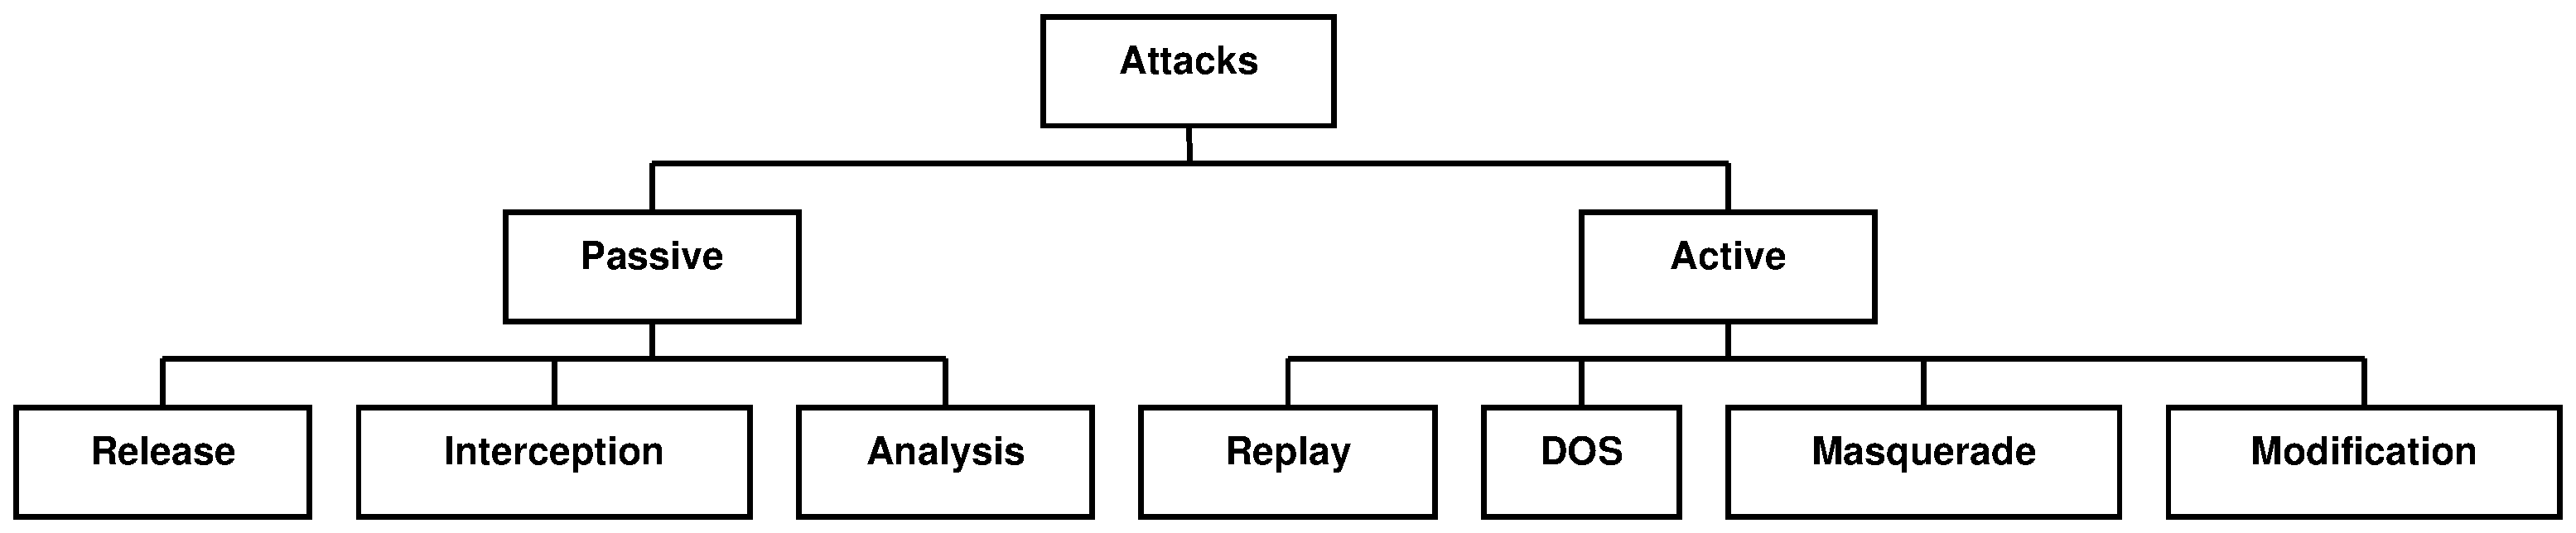
\includegraphics[width=1\textwidth]{figures/attacks.eps}
%     \caption{Classification of attacks}
%     \label{fig:attacks}
% \end{figure}
% The standard model for entity $A$ sending information to entity $B$ is shown in Figure \ref{fig:stdComm}. 
% \begin{figure}[h]
%  \centering
% \begin{tikzpicture}[scale=0.2]
% \tikzstyle{every node}+=[inner sep=2pt]
% \tikzstyle{arrow}=[draw, -latex] 
% \tikzset{
%     pil/.style={
%            ->,
%            thick,
%            shorten <=1pt,
%            shorten >=1pt,}
% }
% \usetikzlibrary{automata,positioning}
% \usetikzlibrary{positioning}
% 
% \node[state,text width=0.8cm,align=center]					at (-40,0)		(a)		{A}; 
% \node[state,text width=0.8cm,align=center]					at (0,0)		(b)		{B}; 
% \path[pil,->] (a)  edge[auto]   node[text width=1cm] {} (b);
% \end{tikzpicture}
% \caption{Communication between two users}
% \label{fig:stdComm}
% \end{figure}
\subsection{Passive attacks}
Passive attacks are aimed against confidentiality. The attacker $E$ intercepts the data transmitted between the two or more entities by monitoring the communication
medium and recording all the traffic. 
\\
After obtaining the data, the attacker can \textbf{release} the data itself to an outside entity. Another way to exploit the data is to \textbf{analyze} them,
allowing the attacker to gain knowledge of some kind of meta data like origin, destination, quantity and frequency of the data flows. 
\\
Because of its passive nature, the data sent are not modified, thus such an attack is hard to detect. Otherwise, encrypting the traffic to gain confidentiality suffices to guard
against the release of data. To guard against traffic analysis is harder because it may be impossible to encrypt some kind of meta data. For example, the destination address of a
message may not be encrypted because routers handling the message must be able to determine the next routing decision based on this address.
Another reason is that some meta information will always be present, like the size of the message or the simple fact that communication between two points has occurred.
\begin{figure}[h]
\centering
\begin{tikzpicture}[scale=0.2]
\tikzstyle{every node}+=[inner sep=2pt]
\tikzstyle{arrow}=[draw, -latex] 
\tikzset{
    pil/.style={
           ->,
           thick,
           shorten <=1pt,
           shorten >=1pt,}
}
\usetikzlibrary{automata,positioning}
\usetikzlibrary{positioning}
\node[state,text width=0.8cm,align=center]					at (-40,0)		(a)		{A}; 
\node[state,text width=0.8cm,align=center]					at (0,0)		(b)		{B}; 
\node[state,text width=0.8cm,align=center]					at (-20,-10)		(e)		{E}; 
\node[state,text width=0.1cm,align=center,minimum size=0.1,fill]		at (-20,0)		(+)		{}; 
\path[pil,->] (a)  edge[auto]   node[text width=1cm] {} (b);
\path[pil,->] (+)  edge[auto]   node[text width=1cm] {} (e);
\end{tikzpicture}
\label{fig:passAttack}
\caption{Passive attack}
\end{figure}
\subsection{Active attacks}
Unfortunately, a restriction to passive attacks only is no realistic assumption for many systems. Whenever the adversary has access to the communication medium, active attacks
cannot be ruled out, allowing the attacker to modify the data stream, or to create false ones. In contrast to their passive counterparts, active attacks can be detected but
not prevented. Therefore, the focus lies on detecting and recovering from active attacks.
\\
\\
\begin{figure}[hf]
\centering
\begin{tikzpicture}[scale=0.2]
\tikzstyle{every node}+=[inner sep=2pt]
\tikzstyle{arrow}=[draw, -latex] 
\tikzset{
    pil/.style={
           ->,
           thick,
           shorten <=1pt,
           shorten >=1pt,}
}
\usetikzlibrary{automata,positioning}
\usetikzlibrary{positioning}
\node[state,text width=0.8cm,align=center]					at (-40,0)		(a)		{A}; 
\node[state,text width=0.8cm,align=center]					at (0,0)		(b)		{B}; 
\node[state,text width=0.8cm,align=center]					at (-20,-10)		(e)		{E}; 
\node[state,text width=0.1cm,align=center,minimum size=0.1,fill]		at (-20,0)		(+)		{}; 
\path[pil,->] (a)  edge[auto]   node[text width=1cm] {} (b);
\path[pil,->] (e)  edge[auto]   node[text width=1cm] {} (+);
\end{tikzpicture}
\label{fig:actAttack}
\caption{Active attack}
\end{figure}
A \textbf{replay} attack consists of two steps: first, the attacker monitors the traffic (i.e., conducts a passive attack) and injects this recorded package in the second step,
thus trying to produce an unauthorized effect.
Of course the package can also be modified and injected afterwards, resulting in a \textbf{modification} attack.
A \textbf{Denial of Service (DOS)} attack tries to overload system resources, attacking availability such that the system is not
usable by legitimate users. Finally, \textbf{masquerade} attacks occurs when one entity pretends to be another entity, often based on replay attacks by replying (modified)
authentication messages of an authorized entity.
\\
\\
To prevent active attacks, integrity mechanisms must be combined with confidentiality mechanisms - 
the basic tool to achieve them is cryptography, introduced in the next Section \ref{sec:crypto}. To provide availability, different techniques must be used,
as shown in Section \ref{sec:availability}.

\section{Cryptography}\label{sec:crypto}
Cryptography\footnote{classical greek for krypt\^{o}s: concealed}
is the science of encrypting information - its evolution was no linear process. Ciphers were used independently in different
places, were forgotten and disappeared when the corresponding civilization died.
A short time table for prominent events is presented below; for a comprehensive outline of cryptographic history, "The Codebreakers", written by David Kahn,
is suggested \cite{codebreakers}.
\\
\\
One of the oldest witnesses for cryptography are hieroglyphs used in Egypt about 2000 B.C., forming the predecessor
of a simple substitution cipher. 500 B.C., the "skytale" was used by greek and spartan military leaders, performing a transposition cipher. Another classical
example is the "Caesar Cipher", named after its inventor and used about 100 B.C. to hide information by replacing every letter of the alphabet by a letter some fixed number down the alphabet,
thus performing a substitution cipher. Ahmas al-Qalqashandi, an egypt writer, introduced the frequency analysis, a method for breaking substitution ciphers,
in the 14th century. About 300 years later, the "Geheime Kabinets-Kanzlei" in Vienna routinely intercepts, copies and 
 re-seales diplomatic correspondence to embassies, and manages to decrypt a great percentage of the ciphertexts. In the beginning of the 20th century, the 
 first cryptographic device called "Enigma"\footnote{classical greek for "riddle"} is patented for commercial use and is later used in World War 2 by german troops for 
 military communication. Successful attacks against the "Enigma" cipher are demonstrated by polish mathematicians even before outbreak of the war, and systematic
 decryption of "Enigma" - based ciphertexts are conducted in Bleatchley Park, U.K., by using so called "Turing-Bombs", giving the allies invaluable advantages.
The second half of the 20th century introduces public key cryptography. In 1976 Whitfield Diffie and Martin Hellman specify a 
protocol for key exchange, based on a public key system developed by Ralph Merkle. One year later, the RSA public key encryption is invented by the american
mathematicians Rivest, Shamir and Adleman.
\\
Cryptography is basically the art of hiding information by turning cleartext
data into a random looking stream or block of bits, called ciphertext, using some kind of
key. This process is referred to as encryption in general, but it is important to note that for many block ciphers, this encryption process
can also be used to generate a special tag called \gls{mac2}, providing integrity.
\\
The next sections deal with how to achieve confidentiality, the 
concepts of how to achieve integrity are partially based on the confidentiality methods and are introduced in Section \ref{Integrity}.
\\
\\
Key, clear- and cipher text are strings built from the alphabet $\mathcal{A}$. 
\begin{itemize}
 \item $\mathcal{A}$ is a finite set, denoting the alphabet used, for example
 $\mathcal{A} = \{0, 1\}$
 \item $\{0, 1\}^n$ denotes the set of all possible strings with length $n$
 \item $\mathcal{M}$ denotes the message space, consisting of all strings that can be built with the 
 underlying alphabet
 \item $\mathcal{C}$ denotes the ciphertext space, also consisting of the strings from 
 the alphbet
$\mathcal{A} = \{0, 1\}$
\item $\mathcal{K}$ denotes the keyspace, also built from the alphabet. Key $e$ is used for encryption, while key $d$ is used for decryption.
Both keys are also referred to as keypair, written $(e,d)$. 
If it is computationally easy to derive the private key $e$ from the public key $d$ (in most cases $e = d$), the encryption scheme
is called symmetric, otherwise the scheme is called asymmetric.

Every element $e \in \mathcal{K}$ determines the function $\mathcal{M} \rightarrow \mathcal{C}$
  \begin{center}
 $ciphertext = E_e(cleartext)$ \footnote{this one-parameter function can also be written as the equivalent two-parameter function $ciphertext=E(e,cleartext$)}
  \end{center}
\end{itemize}
Unauthorized parties - lacking the used key - should, by looking at the ciphertext, learn
absolutely nothing about the hidden cleartext apart from the length of the origin message. Authorized parties are
able to retrieve the original data out of the ciphertext by using the key with polynomial work, thus reversing
the encryption. This reversing process is called decryption.
\begin{itemize}
 \item For every key $d \in \mathcal{K}$, $D_d$ denotes the function from $\mathcal{C} \rightarrow
  \mathcal{M}$, and is called decryption function.
  \begin{center}
  $cleartext  = D_d(ciphertext)$
    \end{center}
\end{itemize}
Combining these properties yields a cipher or encryption scheme defined over $\mathcal{(K,M,C)}$, which is a pair of \textit{efficient}
 \footnote{"runs in polynomial time"} algorithms such that
 \begin{center}
   $\mathcal{K} \times \mathcal{M} \rightarrow \mathcal{C}$
   \\
   $\mathcal{K} \times \mathcal{C} \rightarrow \mathcal{M}$
 \end{center}
 The correctness property ensures for every pair of $(e,d) \in \mathcal{K}$ and for every message $m \in \mathcal{M}$ that encryption is reverseable, i.e., 
 it must hold that 
 \begin{center}  
 $ m = D_d(E_e(m))$
  \end{center}

\subsection{Security of a cipher}

\subsubsection{Perfect secrecy}

A formal definition of a secure cipher was introduced by Shannon in 1949 \cite{6769090}, viewed from a communication-theory point of view, as follows:
given a finite message space, every possible cleartext message has its own a priori probability (for example, the distribution of letters in a 
specific language). Additionally, every key can be chosen with specific probability. It is assumed that these
two probabilities constitute the a priori knowledge of an attacker.
\\
A message is picked, encrypted
and sent to the receiver. The eavesdropper, intercepting the message, can calculate the a posteriori probabilities for all possible cleartext messages, 
leading to the observed cipher text - these are the conditional properties that under a fixed key, encrypting the cleartext message lead to the
observed ciphertext message.
\\
If the a posteriori probabilities for all possible encryptions are the same as all a priory probabilities, the attacker has learned absolutely
nothing from intercepting the cipher text, which is defined by Shannon as "perfect secrecy". Such a cipher cannot be broken by a ciphertext-only-attack,
even by an adversary with unlimited time and processing power.
\\
Shannon proved that for a perfectly secure cipher, the key space must be at least as big as the message space.
Otherwise there will exist cleartext messages which are mapped to the same cipher texts, and thus a priori and a posteriori probabilities will be different,
allowing the attacker to get knowledge he should not have gotten. 

\subsubsection{Semantic security}

Another definition of the security of a cipher, based on complexity theory, is "semantic security".
To be semantically secure, a cipher must not be breakable by an adversary in a reasonable time
frame \cite{handbook1}, where this time frame is a function of the useful timespan of the protected data. This synonymously means for a semantically secure
cipher that an adversary must be forced to spend super-polynomial time to be able to break it. It follows that \textit{all} semantically secure ciphers
can be broken in principle by mounting the "brute-focrce" attack, searching the correct $n$-bit key in the exponential big key space $2^n$. Thus, such an
exhaustive search must be rendered impracticable by using a suitable large key space to obtain a secure cipher.
Semantic security is therefore a weaker form of security, namely perfect secrecy against an adversary having only polynomially bounded
processing powers \cite{GoldwasserMicali}.

\subsubsection{Kerckhoff's principle}
When designing cryptographic systems, a fundamental question is what components of it have to be protected from public knowledge, and what parts can be
published without compromising the security of the system. 
\\
The dutch cryptographer Auguste Kerckhoff stated rules for designing a secure cipher.
According to "Kerckhoff's Principle" that was stated in the year 1883, among other properties, a secure system should not rely on the secrecy of
its components, the only part that should be kept secret is the key alone. Shannon acknowledged these assumptions to be "pessimistic and hence safe, but 
in the long run realistic, since one must expect the system to be found out eventually".
\\
\\
Mapped to the definitions above, the sets $\mathcal{M, C, K}$, as well as the
transformation functions $E_e$ and $D_d$, must not be secret. The only thing that has to be kept private is the decryption key $d$.
This separation of key and algorithm allows the publication of the basic cipher methods, benefiting from peer review. A contradicting approach 
trying to strengthen the safety of a cryptographic system by hiding the inner workings from public is also known as "Security by Obscurity".

\subsection{Randomness and probabilistic theory}
A basic requirement of all cryptographic schemes is the availability of randomness. Entropy, denoted $H$, is the unit of the unpredictability of a process, as
 defined by Shannon in \cite{6773024}
 \begin{align}
 H = - \sum_{i=1}^{k} p_i* ln(p_i)
\end{align}
where $p_i$ is the probability of a certain outcome.
The higher the predictability, or in other words, the more likely an event, the lower its entropy. Flipping a "fair" coin is a canonical 
example of a process with maximum entropy, because every coin flip has a probability of $\frac{1}{2}$, and all flips are independent from each other \cite{1621063}.
If obtaining "heads" of the coin is viewed as a logical "0" and "tails" as a logical "1", a binary string of length $n$ can be built, where the probability of all possible
strings of same length is equal, as shown in Figure \ref{fig:uniform}, yielding a uniform distribution, with
$H = 2^n*\frac{1}{2^n}*ln(2^n) = n$ bit. 
\\
\\
The importance of random numbers in cryptography is founded on the nature of the cipher used, as will be shown in the next sections. For example,
stream ciphers generate a keystream which is used
for encryption. If the keystream is predictable by an adversary, the security of the cipher is reduced. Similar arguments are valid for block ciphers, which often
rely on an initial value called \gls{iv} for encryption. Key negotiation algorithms schemes often rely on finding a random prime number, which can be 
achieved by choosing a random number and testing it for primality. Again, if such a prime number can be narrowed down within some borders, this fact may
weaken the encryption process.
\\
A fundamental problem in generating random numbers by utilizing computing devices is the deterministic nature of an algorithm:
\\
\\
\textit{"Anyone who considers arithmetical methods of producing random digits is, of course, in a state of sin."} \footnote{John von Neumann, 1951}
\\
\\
Such numbers are therefore called \textit{pseudo}random. Lots of cryptographic products suffered serious flaws because of relying on a broken \gls{prng}. A 
historical example of such a broken random number generator, outputting biased (i.e., not uniformly distributed) values was "RANDU", invented by IBM in the
1960s. 
The generator belongs to the class of multiplicative congruential algorithms as proposed by Lehmer \cite{MR0044899}, which can basically generate random
numbers of sufficient quality, \textbf{if} the parameters are chosen correctly.
Random values can be obtained after setting an initial value for $I_0$, called seed, and repeatedly executing the calculation
\begin{center}
 $I_{j+1} = 65539 * I_j \pmod{2^{31}}$.
\end{center}
One problem 
is that consecutive values generated by RANDU are not independent, a fact that	 can be seen in Figure \ref{fig:randu}. To obtain the plot, 10000 uniformly distributed 
random numbers were chosen as initial seeds for $I_i$ and plotted as x-values, $I_{i+1}$ served as y- and $I_{i+2}$ as z-values. While one would suspect that all points
would be equally distributed, a clear pattern arises, indicating that the values are correlated.
\\
To assess the quality of a \gls{prng}, beside of such spectral tests lots of additional tests are available, see \cite{nistRAND} for details.
\\
To encounter the shortcomings of a \gls{prng}, a \gls{trng} uses a natural process as non-deterministic data source, for example
thermal noise of a semi conductor, cosmic noise from space or digital oscillators.
\begin{figure}
    \centering
    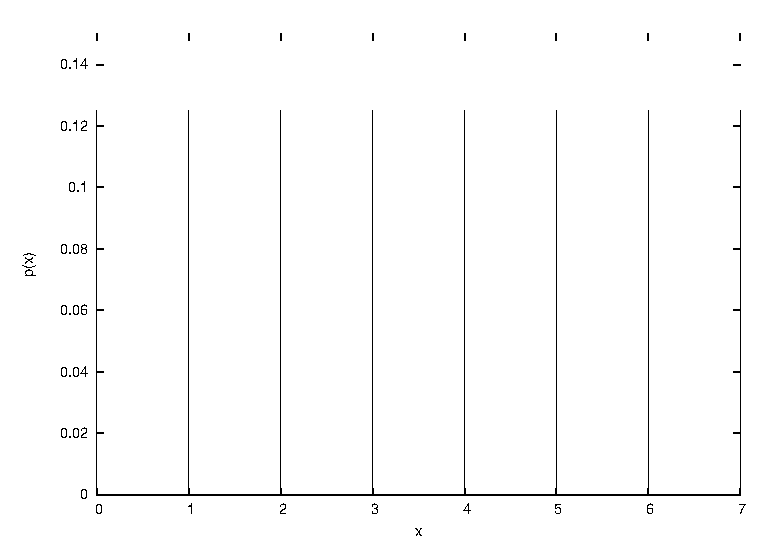
\includegraphics[width=0.6\textwidth]{figures/uniform}
    \caption{Uniform Distribution of binary string of length three}
    \label{fig:uniform}
\end{figure}
\begin{figure}
    \centering
    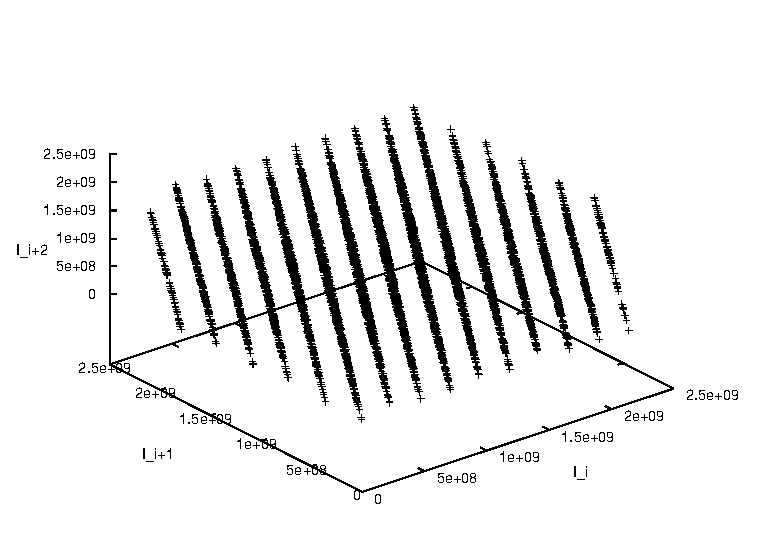
\includegraphics[width=1\textwidth]{figures/randu}
    \caption{Spectral Plot of RANDU output}
    \label{fig:randu}
\end{figure}

\subsection{The discrete logarithm problem}\label{refDLP}
The \gls{dlp}, a mathematical problem, is the basis of two important key exchange algorithms, both introduced in Section \ref{pkc}. \gls{dh} utilizes finite fields, whose
theoretical background is introduced below. \glspl{ec}, basis for the second algorithm, are also explained.

\subsubsection{Finite fields \gls{dlp}}
A field consists of a set $\mathcal{F}$ together with two operations $\cdot$, namely addition "+" and multiplication "*", satisfying the following properties:
\begin{itemize}
 \item  Closure: for all elements from $\mathcal{F}$, the set is closed under the defined operations, i.e., applying an operator $\cdot$ to two elements from the set results in an
element also belonging to the set.
 \item Associativity and commutativity hold, i.e., $a \cdot (b \cdot c) = (a \cdot b) \cdot c$ and $a \cdot b = b \cdot a$
 \item For both operations, an identity element $e$ exists such that $a\cdot e = a$  for all elements from the set $\mathcal{F}$ 
 \item For both operations, an inverse element exists such that $a\cdot a^{-1} = e$ for all elements from the set $\mathcal{F} \backslash \{0\}$ 
 \item Distributivity holds: $(a+b) \cdot c = a \cdot c + b \cdot c$ for all elements 
\end{itemize}
For a finite field, the cardinality of the set 
$\mathcal{F}$ is finite and called order of the field, with identity elements for addition and
multiplication. Inverses can be found for all
elements regarding addition such that $a + (-a) = e$ and regarding multiplication for all elements except ${0}$ such that $a * a^{-1} = e$.
\\
\\
A specific example of a finite field is a prime field, which can be constructed by taking the set of integers $\mathbb{Z}\pmod p$, with $p \in \mathbb{P}$, thus
restricting the set of all integers to the set $\mathbb{Z}_p = \{0, 1, ..., p-1\}$.
By choosing $p$ as prime it is ensured that for any element $a \in \mathcal{F} \backslash\{0\}$, a multiplicative inverse exists: $ a * a^{-1} = 1 \pmod p$.
The set of numbers for which multiplicative inverses exist is called $\mathbb{Z}{_p}^*$, so for $p$ being prime, $\mathbb{Z}_p \backslash \{0\} = \mathbb{Z}{_p}^*$.
\\
By raising an element $a \in \mathbb{Z}_p$ to different powers, a subgroup of $\mathbb{Z}{_p}^*$
is generated, a fact that follows from Fermat's little theorem stating that for $p$ being prime and raising $a$ to the power $p-1$, the outcome is congruent 1
modulo p
\begin{center}
 $a^{p-1} \equiv 1 \pmod p $.
\end{center}
Raising $a$ to higher powers results in
\begin{center}
 $a^{p} \equiv a*a^{p-1} \equiv a \pmod p$ \\
 $...$ \\
 $a^{2p} \equiv a^2 * a^{p-1} * a^{p-1} \equiv a^2 \pmod p$.
\end{center}
Thus, generating higher powers than $(p-1)$ does not yield different outcomes. If by raising $a$ to $(p-1)$ different powers all elements from $\mathbb{Z}{_p}^*$ can
be generated, $a$ is called primitive root or generator, generating a cyclic group.
If $p$ is prime it can be shown that at least one such generator $g$ must exist and can be found efficiently \cite{primitiveRoot}.
Conversely this means that for all elements from  $\mathbb{Z}{_p}^*$ a unique exponent in the interval $[0, p-1]$ exists,
called the discrete logarithm for the base $ g \pmod p$.
\\
\\
Several algorithms exist to find the discrete logarithm.
The most naive method conducts an exhaustive search, so for a prime of $n$ bits length, $2^n$ search operations
are necessary. More efficient algorithms exist, with the best methods finishing after about $2^{\frac{n}{2}}$ steps \cite{5199978}. 
Therefore, by choosing a sufficient large prime, finding the discrete logarithm is considered a hard problem, a fact
that is exploited by the \gls{dh} key exchange algorithm and its variants.

\subsubsection{Elliptic curve \gls{dlp}}\label{sec:ecIntro}
An \gls{ec} is basically the set of all points
satisfying an equation with the form as shown in \ref{basicEC}, called "Weierstraß" equation
\begin{align}\label{basicEC}
 y^2 = x^3 + ax +b
\end{align}
The additional condition $4a^3 + 27b^3 \neq 0$ assures that the \gls{ec} does not possess any singularities.
\\
An imaginary point "in infinity", denoted $\infty$, serves as additive identity element, and also belongs to the \gls{ec} by definition
\begin{center}
 $P + \infty = \infty + P = P, P + (-P) = \infty$.
\end{center}
Negatives can be calculated easily due to the symmetric nature of the curves by swapping the sign of the y-coordinate of the point. For point $P$ with coordinates $(x, y)$, $-P$ is defined as
$(x,-y)$, thus satisfying $P + (-P) = \infty$.
\\
By defining an \gls{ec} over $\mathbb{Z}_p$, with $a, b \in \mathbb{Z}_p$, a cyclic group can be generated. The addition operation that "adds" two points on
this curve is defined by a "chord-and-tangent" rule. Figure \ref{fig:ecAdd}
shows addition of two points, while \ref{fig:ecDouble} shows adding a point to itself. It is important to note that this representation is shown in the domain
$\mathbb{R}$ for visualization - in real \gls{ec} cryptography, only elements $\pmod p$ (i.e., from the set $\mathbb{Z}_p$)
are allowed to avoid rounding errors. 
\\
\\
Addition is defined as connecting points $P$ and 
$Q$, finding the intersection of the line with the \gls{ec} ($R'$) and reflecting that point across the x-axis to obtain the result $R$. 
%\begin{minipage}{\linewidth}
%      \centering
%      \begin{minipage}{0.8\linewidth}
          \begin{figure}[H]
          \centering
              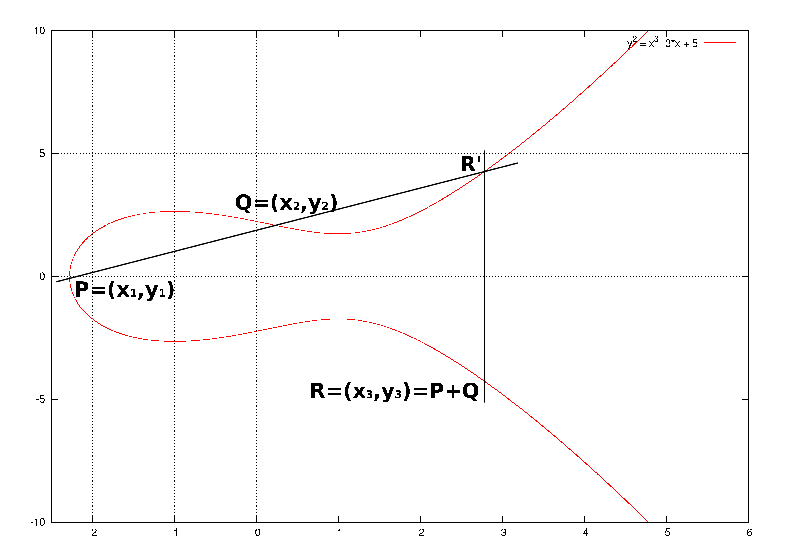
\includegraphics[width=0.6\linewidth]{figures/ecAdd.eps}
              \caption{Adding two points}
              \label{fig:ecAdd}
          \end{figure}
Mathematically, the new coordinates can be calculated as shown in equation \ref{adding}
\begin{align}\label{adding}
x_3 = (\frac{y_2-y_1}{x_2-x_1})^2-x_1-x_2, y_3=\frac{y_2-y_1}{x_2-x_1}(x_1-x_3)-y_1.
\end{align}   
Point-doubling of $P$ is achieved in a similar way by determining the tangent of $P$, finding the intersection and reflection.
%      \end{minipage}
     % \hspace{0.05\linewidth}
%      \begin{minipage}{0.8\linewidth}
          \begin{figure}[H]
	    \centering
              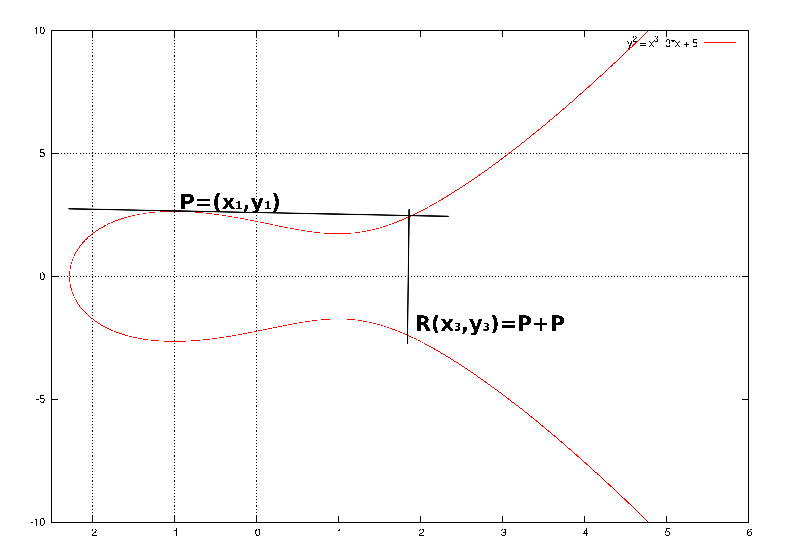
\includegraphics[width=0.6\linewidth]{figures/doubleEC.eps}
              \caption{Doubling a point}
              \label{fig:ecDouble}
          \end{figure}
%      \end{minipage}
%  \end{minipage}
% Formulae to calculate x- and y-coordinates for the resulting points
% for point addition $R=P+Q$ and point doubling $R=P+P$ are shown in equations \ref{adding} and \ref{doubling} respectively:
% 
% 
% \begin{align}\label{doubling}
%  x_3 = (\frac{3x_1^2 +a}{2y_1})^2 - 2x_1, y_3=\frac{3x_1^2+a}{2y_1}(x_1-x_3)-y_1
% \end{align}
Multiplication is defined as successive addition of a point to it self in the way
\begin{center}
 $kP = \underbrace{P+P+...+P}_{k-times}$.
\end{center}


\subsubsection{\gls{ecdlp}}\label{ecdp}

Based on this group operations, the \gls{ecdlp} \cite{ecdlp} can be defined as follows: given an \gls{ec} $E$ over the finite field $\mathcal{F}_p$, $P$ of order $n$ of this curve 
and a point $Q$, find the integer $k$ such that $Q = kP$. $k$ is called the discrete logarithm of $Q$ to the base $P$.
\\
\\
To find $k$, the most naive algorithm trying all possible numbers will terminate after $\frac{n}{2}$ on average. In contrast, the running time of the best known attack is bounded by 
$\sqrt{p}$, where $p$ is the largest prime divisor of $n$. Therefore, such an attack is infeasible for properly chosen \gls{ec} parameters.
%Additionally to the CIA - triad, sometimes two more concepts are used in the security field: \textbf{Authenticity} is tied to integrity and ensures the property
%of being genuine, while \textbf{Accountability} allows to link actions performed on a system uniquely to the entity responsible for them.

\section{Symmetric vs. Asymmetric Cryptography}

As already stated, two very fundamental differences regarding the key used in a cryptographic system can be found. Symmetric ciphers, where 
the same key is used for encryption and decryption, outperform its asymmetric counterparts in regards of data throughput by a factor of about 1000 \cite{5412055}.
Additionally, they need shorter keys to achieve the same level of security - both arguments encourage its use in embedded devices because of its less computing
and memory demands.
\\
The big disadvantage of symmetric ciphers is that the key must be known to sender
and receiver of the message \textit{before} secure communication can take place. This constitutes some kind of chicken-egg problem: to be able to send encrypted
data, the key must be distributed, i.e. a secure channel has to be setup first for key exchange. But if such a secure channel can be established, it could also be used
for transmitting the sensitive data themself.
\\
Asymmetric or public key cryptography solves the problem of key distribution by using two different keys, belonging to the same key pair: the \textit{private}
key must be be protected from disclosure, while the \textit{public} key can be published without harming security. For encryption, the public key of the receiver
is used, who in turn will use his private key to decrypt the message. 
\\
To be able to take benefit from the advantages of both schemes, a hybrid approach is possible: at first, public key cryptography is used to negotiate a symmetric session
key, which then can be used to encrypt the actual, sensitive data.

\subsection{Stream Ciphers}
Most stream ciphers belong to the family of symmetric ciphers, thus $e_i = d_i$. The reason is that most asymmetric ciphers are deterministic ciphers,
i.e. the encryption of the same message with a fixed public key always yields the same cipher text. Thus, such repeated messages can be detected by 
an adversary. 
Probabilistic public-key encryption can solves this problem for stream ciphers,
but this scheme will not be handled in this work because of its low practical application.
\\
For encryption, stream ciphers take arbitrary long messages (from the message space $\mathcal{M}$), and encrypt
them to the corresponding ciphertext (out of the ciphertext-space $\mathcal{C}$), by applying
one digit of the message to one digit of the key. It is valid to say that a streamcipher is a block cipher with blocklength 1.
\begin{itemize}
 \item A keystream is a sequence of symbols $e_0, e_1, ..., e_n$, all taken from the keyspace $\mathcal{K}$
\end{itemize}
The encryption function $E_e$ performs the substitution $c_i = E_e(e_i, m_i)$, producing one encrypted symbol at a time. Analogously,
the decryption function inverts this substitution: $m_i = D_d(d_i, c_i)$.

\subsubsection{The Vernam Cipher} 

This cipher, also called \gls{otp}, was invented by Gilbert Vernam in 1918, and belongs to the family of polyalphabetic stream ciphers,
which means that every character of the origin message is mapped to another character of the same alphabet. In contrast to a monoalphabetical cipher,
there is no fixed mapping between the input and output characters.
The substitution is achieved by generating a keystream and by executing 
a bit-wise \gls{xor} operation, as defined in table \ref{table:xor}, of key and message.
\begin{center}
\begin{tabular}{ c c | c }
 \label{table:xor}
   &  & $\bigoplus$ \\ \hline
  0 & 0 & 0 \\
  0 & 1 & 1 \\
  1 & 0 & 1 \\
  1 & 1 & 0 \\
\end{tabular}
\end{center}
Decryption can be achieved by applying the \gls{xor} operation to key and ciphertext:
\begin{center}
 $m_i = c_i \bigoplus k_i = (m_i \bigoplus k_i) \bigoplus k_i = m_i$, with $ k_i \bigoplus k_i = 0, const \bigoplus 0 = const$
\end{center}
Obviously, the security of the cipher heavily depends on the quality of the \gls{prng}. If a truly random source is used to generate the key stream, this cipher
has perfect secrecy: for a n-character ciphertext, \textbf{all} n-character cleartexts are equally probable, and vice versa. 
The reason for this is the \gls{xor} operation: both outcomes are equally probable, introducing one bit of randomness into every data bit. 
\\
Additionally, the \gls{xor} operation can be built easily in hardware, accelerating the encryption or decryption process.
\\
Nevertheless, the cipher can be completely broken if the same key is used for encrypting more than one cleartext message, allowing to mount
an attack based on frequency analysis.
If an attacker is able to intercept a high number of different ciphertexts, all encrypted with the same key, the pairwise xor'ing of the ciphertexts
yields the xor-combination of the corresponding cleartexts, because
\begin{center}
 $m_1 \bigoplus m_2 = (c_1 \bigoplus k) \bigoplus (c_2 \bigoplus k) = c_1 \bigoplus c_2 \bigoplus k \bigoplus k = c_1 \bigoplus c_2 \bigoplus 0 = c_1 \bigoplus c_2$
\end{center}
Whenever the same character is present in two different ciphertexts at the same position, the result of the \gls{xor} operation will be 0x00, allowing to draw
inferences about the language used. By utilizing frequency analysis, the used key can be determined with high probability position by position with effort bounded by $O(n^2)$.

\subsubsection{Stream Ciphers based on \gls{lfsr}}

An disadvantage of the Vernam cipher is that a key of equal length as the message is necessary. To mitigate this problem, a \gls{lfsr} can be used to generate
a key of proper length from a much shorter, initial key, called \textit{seed}. Such \gls{lfsr} are denoted by the tuple $\langle L, C(D) \rangle$. $L$ is the number of stages, and $C(D)$ is the
\textit{connection polynomial}. Because of the finite length, every \gls{lfsr} can only take on a finite number of internal states, producing
a periodic output sequence.
If the degree of the connection polynomial is equal to the number of stages and the connection polynomial is irreducible (i.e. the polynomial can not
be factored into 2 non-constant polynomials), no matter of the initial state, the output sequence produced will always be of maximum periodicity.
\\
Figure \ref{fig:lsfr} shows a 4 stage non-singular \gls{lfsr} with
\begin{center}
 $L=4$,  $C(D) = 1 + D + D^4$,
\end{center}
Table \ref{table:lfsr} \cite{handbookLFSR} shows the corresponding output sequence produced. After
15 shifts a state equal to the initial state is achieved, and the outputs
begin to repeat.
\\
While such \gls{lfsr} can be easily built in hardware, a problematic fact remains that their \textit{linear complexity} is bounded by $L$. Therefore, a \gls{lfsr}
should never be used as keystream generator directly, instead the outputs of different \gls{lfsr} are combined by a non-linear function, thus obtaining a
nonlinear generator.
\begin{figure}
    \centering
    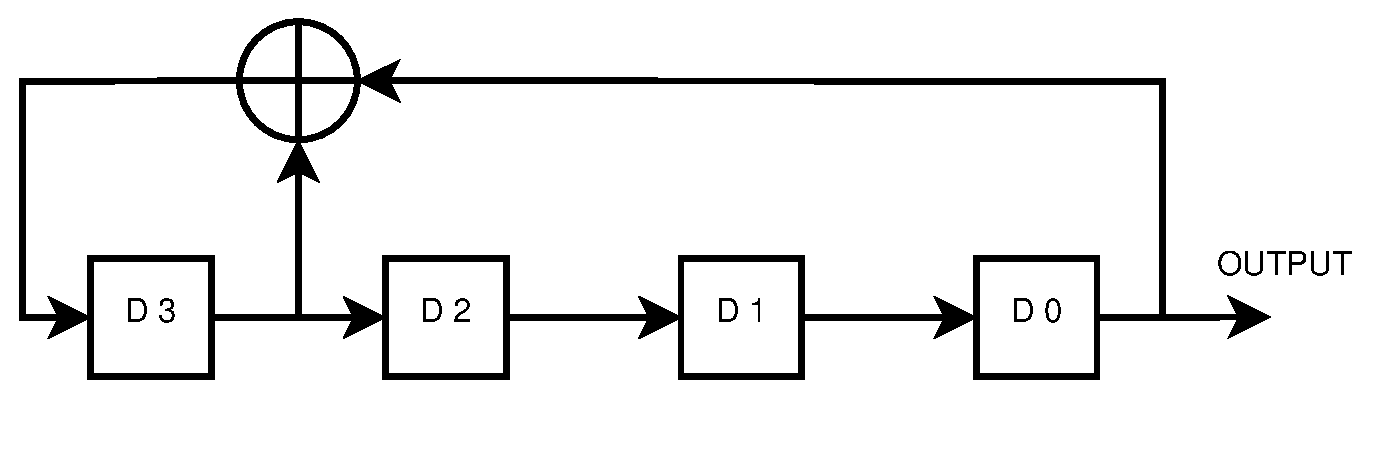
\includegraphics[width=0.8\textwidth]{figures/LSFR.eps}
    \caption{4 Stage LFSR}
    \label{fig:lsfr}
\end{figure}
\begin{center}
\begin{minipage}{0.45\textwidth}
\begin{tabular}{ c | c | c | c | c }
 \label{table:lfsr}
  t & $D_3$ & $D_2$ & $D_1$ & $D_0$ \\ \hline
  0 & 0 & 1 & 1 & 0 \\
  1 & 0& 0& 1& 1\\
  2 & 1&0 &0 &1 \\
  3 & 0& 1& 0& 0\\
  4 & 0&0 &1 &0 \\
  5 & 0&0 &0 &1 \\
  6 & 1&0 &0 &0 \\
  7 & 1&1 &0 &0 \\
  \end{tabular}
\end{minipage}\hfill
\begin{minipage}{0.45\textwidth} 
\begin{tabular}{ c | c | c | c | c }
  t & $D_3$ & $D_2$ & $D_1$ & $D_0$ \\ \hline
  8  & 1& 1& 1& 0\\
  9  & 1& 1& 1& 1\\
  10 & 0& 1& 1& 1\\
  11 & 1& 0& 1& 1\\
  12 & 0& 1& 0& 1\\
  13 & 1& 0& 1& 0\\
  14 & 1& 1& 0& 1\\
  15 & 0& 1& 1& 0\\
\end{tabular}
\end{minipage}
\end{center}

\subsection{Block Ciphers}
These ciphers operate on input blocks of fixed size, transforming them into output blocks of same size. This implies that larger messages must be broken into
suitable blocks, and that for the last remaining block it may be necessary to add padding bytes to yield the full block size,
adding overhead to the message - a disadvantage compared to stream ciphers. For example, to encrypt a message just exceeding the block size by one byte,
for the excess byte a complete block must be concatenated. 
\\
On the other hand, while stream ciphers are strictly sequential by nature, there exist methods to speed up block ciphers by splitting the message
first, and then process them in parallel\footnote{Counter Mode, see \ref{confidentiality}}. 
\\
Two main types of block cipher exist: \textit{transposition} ciphers use a key-dependent permutation to re-order the characters of the block to obtain the ciphertext.
This is a bijective transformation, so decryption can be achieved by simply reversing the permutation.
\\
Substitution ciphers define a key-dependent mapping of characters from the alphabet $\mathcal{A}$ to the same alphabet, thus replacing every character by one
or more other characters. In the latter case, this equals an injective function which can not be reversed directly.
\\
A product cipher is a combination of ciphers of different types to achieve a higher level of security than possible as with the basic ciphers. 
\\
Feistel networks are special product ciphers, composed of \gls{sp} networks. They were first described by Horst Feistel in the year 1973\cite{feistel}, and are 
the basis of a variety of block ciphers like "LUCIFER" \cite{feistel1974block,}, developed by Feistel, and \gls{des}.
\\
Figure \ref{fig:feistel} shows the principal layout of such ciphers: at first, the plaintext block of length
2n-bits is divided into two n-bits blocks, often called $L_0$ and $R_0$ for left and right block, respectively. After that the first round starts: every round
is characterized by performing a substitution, followed by a permutation of the two half-blocks. For substitution, at first a \textit{round function},
parametrized by a \textit{round key} is applied to one half of the data block, followed by a \gls{xor} operation. The output of the rounds can be calculated
according to the formulas shown in \ref{table:feistel}
\\
\begin{center}
\begin{tabular}{ l l}
 \label{table:feistel}
  Encryption of round 1: & $L_1 = R_0$  \\ 
   &  $R_1 = L_0 \bigoplus F(k_1, R_0)$\\ \hline
  Encryption of round 2: & $L_{2} = R_1$  \\
   &  $R_{2} = L_1 \bigoplus F(k_2, R_1)$ \\ \hline
   ... &  \\ \hline
   Encryption of round n: & $L_{n} = R_{n-1}$ \\
   & $R_n = L_{n-1} \bigoplus F(k_n, R_{n-1})$ \\
\end{tabular}
\end{center}
Decryption is achieved by applying the ciphertext to the same network, with the round keys applied in reverse order, reducing hardware- respectively
code size. Because every decryption step, see \ref{table:feistelRev}, does not rely on reversing the round function, there is no necessity for the round function to be bijective.
\begin{center}
\begin{tabular}{ l l}
 \label{table:feistelRev}
Decryption of round n: & $R_{n-1} = L_n$  \\
 & $L_{n-1} = R_n \bigoplus F(k_n, R_{n_1}) = R_n \bigoplus F(k_n, L_{n}) $
\end{tabular}
\end{center}

\begin{figure}
    \centering
    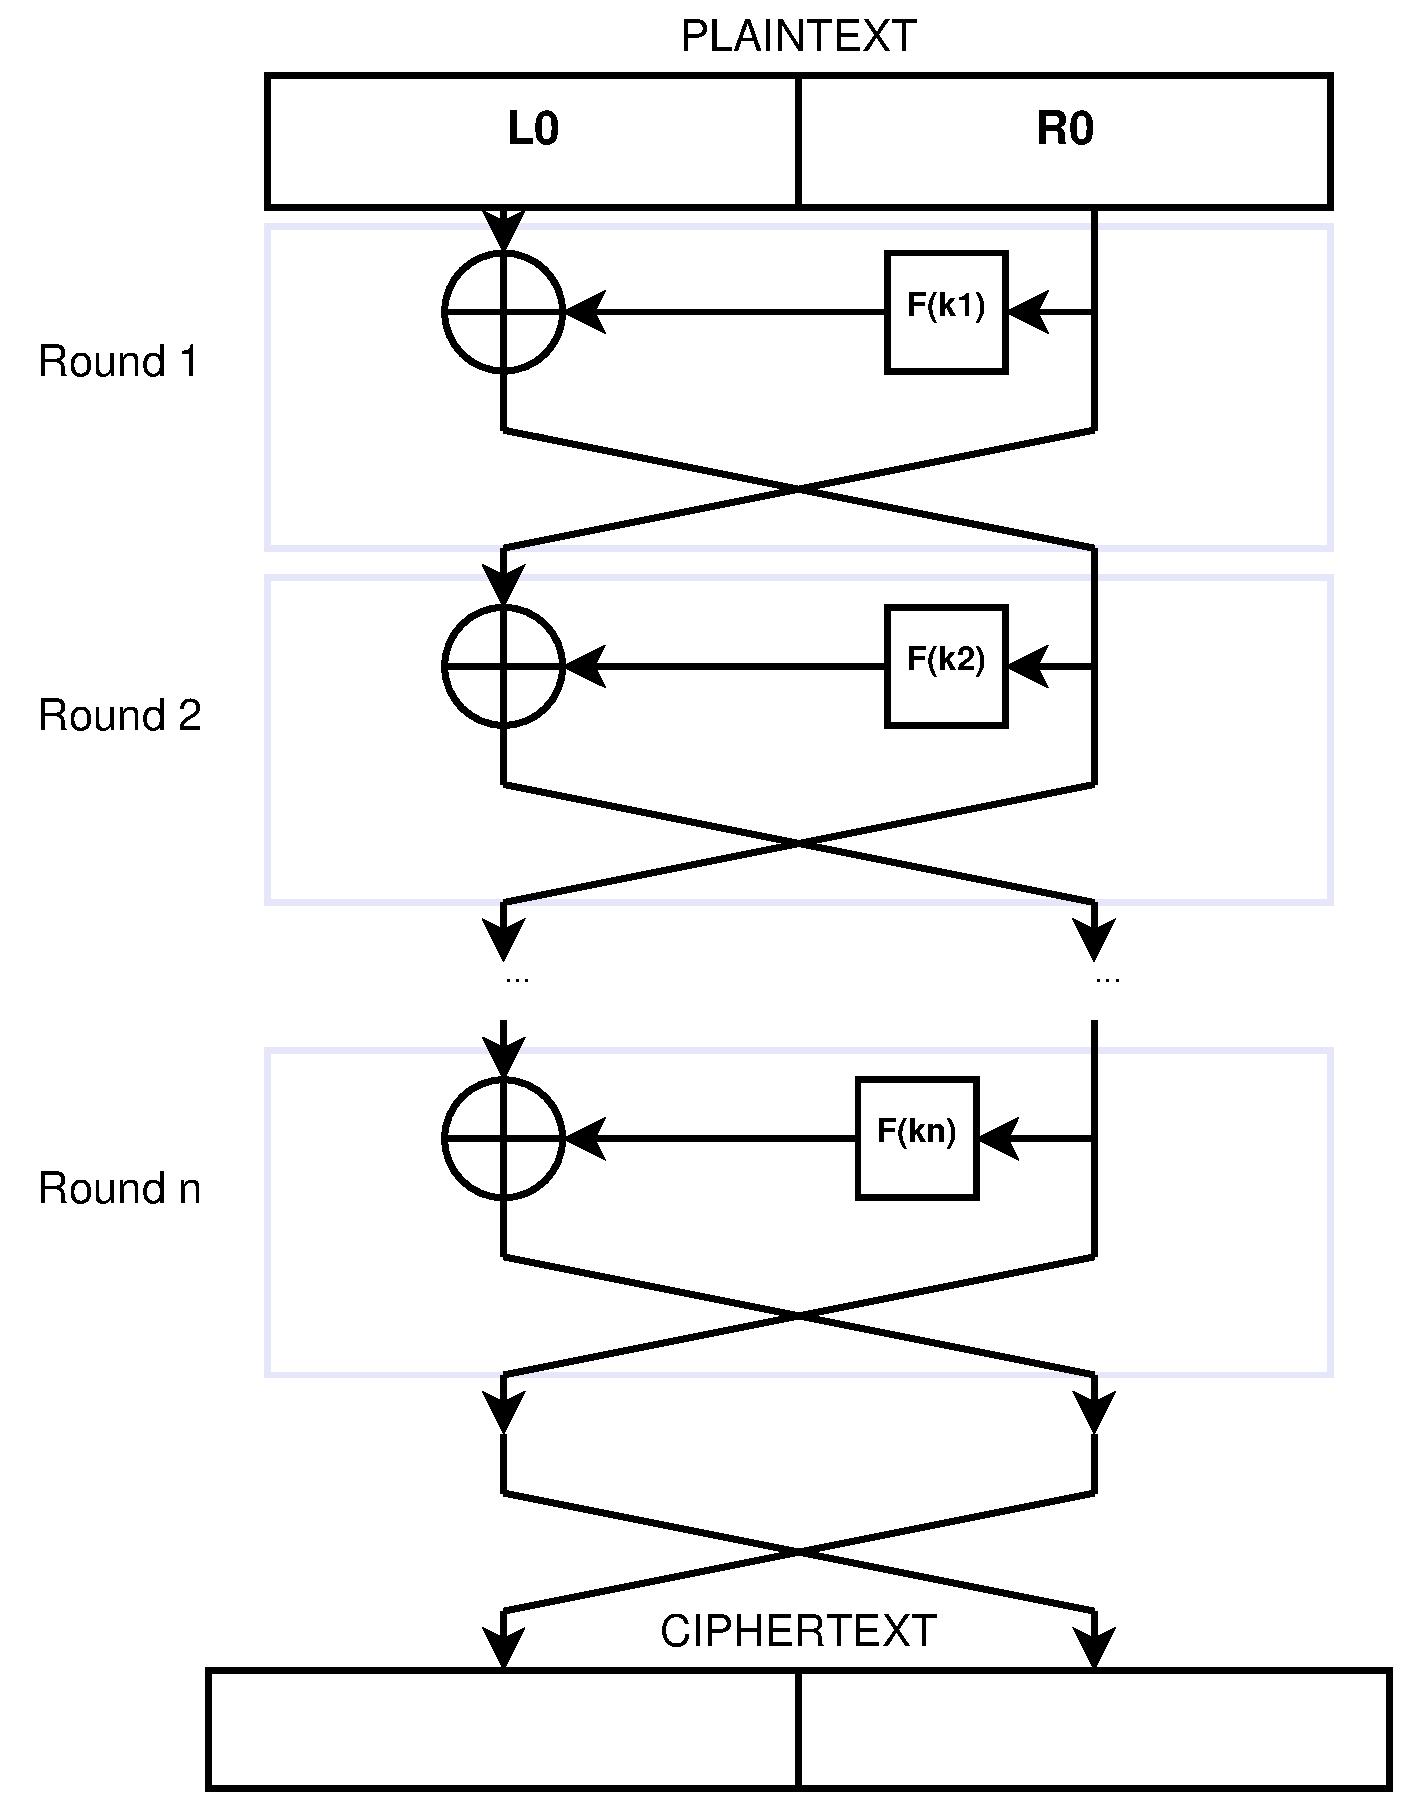
\includegraphics[width=0.5\textwidth]{figures/feistel.eps}
    \caption{Feistel Substitution-Permutation Network}
    \label{fig:feistel}
\end{figure}

\subsubsection{\gls{des} and \gls{3des}}
\gls{des}, designed by IBM and published by \gls{nist} in 1977 \cite{des}, encrypts 64 bit blocks in 16 processing rounds.
\\
For every round, a 56 bit round key is derived from the basic 56 bit
key by permutations. The 64 bit data block to be encrypted respectively decrypted is subjected to an initial permutation and then feed into the Feistel
network. The round function operates as follows:
\\
At first, the 32 bit half block is expanded to 48 bit by copying specific bits. The outcome is added to the round key modulo 2 (i.e., the \gls{xor} operation).
Next, a non-linear transformation is applied by so-called "S-Boxes", performing a surjective function by substituting blocks of 6 bit by only
4 bit. Lastly, a deterministic permutation follows, achieved through "P-Boxes", concluding the round
function.
\\
Because of the small key size, \gls{des} was successfully broken for the first time\footnote{At least officially - rumors about the involvement of the \gls{nsa}
regarding the small key size and the design of the S-Boxes existed since the publication} by a brute-force attack in 1997.
\\
To prevent such attacks, \gls{3des} was published: the cleartext- respectively 
cipertext block is feed 3 times to the \gls{des} cipher, using 3 different keys $k_1, k_2, k_3$ to first encrypt with $k_1$, decrypt with $k_2$ and finally 
encrypt with $k_3$, effectively tripling the key size:
\begin{center}
 $ciphertext = E(k_3(D(k_2,E(k_1, cleartext)))$
\end{center}
The special sequence of encryption, decryption and again encrypting was chosen because by setting $k_1 = k_2 = k_3$, a \gls{3des} implementation can also be used
for en/decryption of \gls{des} messages.

\subsubsection{\gls{aes}}

Also called "Rijndael" after its developers Joan Daemen und Vincent Rijmen, \gls{aes} is is the successor of \gls{3des}, as
proposed by the \gls{nist} in 2001. Basic properties are a block size of 128 bit, and possible key sizes
of 128, 192 or 256 bit.
\\
The operation, shown in Figure \ref{fig:aesEnc}, starts by copying the input block into a square matrix, called "State",
followed by a \gls{xor} combination of the first round 
key and the matrix. Then, 9, 11 or 13 rounds, depending on the key size, are performed: substitution by S-Boxes, permutation by shifting rows, 
another substitution by mixing columns and applying the round key. A last round, omitting the mix-columns stage, concludes the encryption.
Operating on the whole data block, \gls{aes} is not a Feistel network, therefore all substitutions and permutations must be reversible to allow decryption: 
the S-Box used here is therefore implementing byte-by-byte substitutions. The round keys are derived from the origin key by the \gls{aes} key expansion.
\begin{figure}
    \centering
    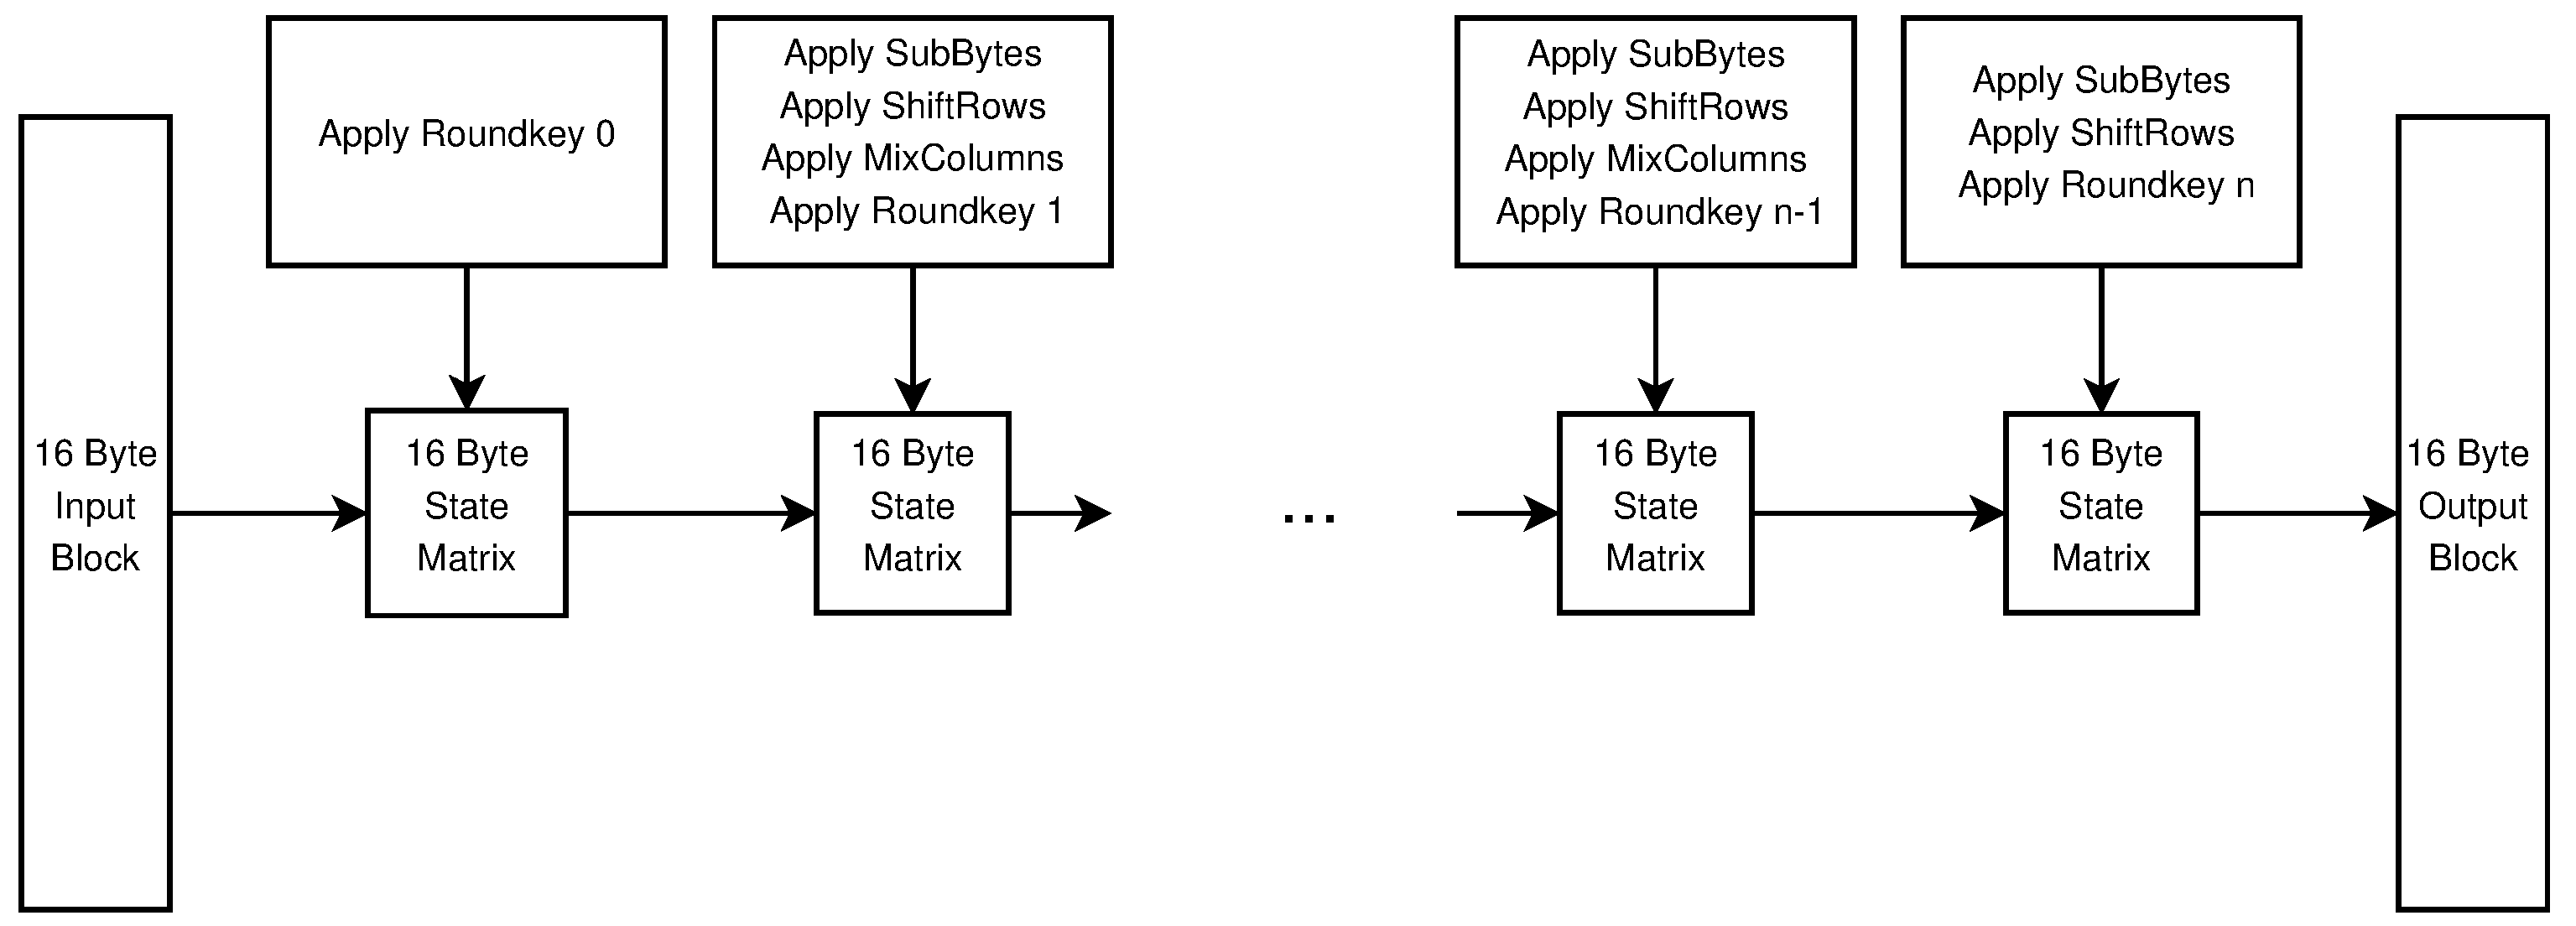
\includegraphics[width=1\textwidth]{figures/aesEnc.eps}
    \caption{AES Encryption Process}
    \label{fig:aesEnc}
\end{figure}
Decryption uses the round keys in reverse order. To reverse the first substitution of every round, a unique inverse S-Box is used, while the shifting rows
and mixing columns can also be reversed.

\subsection{Mode of Operation}\label{confidentiality}

Because block ciphers  operate on a fixed number of bytes, messages larger than this block size must be broken into parts of suitable size, and depending on 
the resulting size of the last block, it may be necessary to append a padding to it. Five different such modes were defined by \gls{nist} in 2001 \cite{moo},
which will be introduced in the next sections. For all modes it does not matter what underlying block cipher is used, as long as the block cipher implements
a cryptographic secure function. 
\\
An important property of this modes is the error propagation.
Whenever a bit error occurs on the transmission channel due to noise or interference,
a logical '0' of the transmitted cipher text is substituted by a logical '1' or vice versa. This bit error in the cipher text produces one or more bit errors
in the clear text, thus the name error propagation \cite{burda}.

\subsubsection{\gls{ecb}}\label{deterministicEnc}

\gls{ecb} can be used to gain confidentiality and allows the parallel processing of all input blocks. This mode does not use any \gls{iv} or nonce, therefore
repeating input blocks are mapped to the same output blocks under the same key, implementing a deterministic encryption scheme.
This is problematic, which can be seen quite intuitively by comparing 
Figures \ref{fig:tuxclr} and \ref{fig:tuxecb}. Therefore, this mode should never be used.
\\
 \begin{minipage}{\linewidth}
      \centering
      \begin{minipage}{0.4\linewidth}
          \begin{figure}[H]
              
\includegraphics[width=\linewidth]{figures/TuxCleartext.png}
              \caption{Unencrypted Picture}
              \label{fig:tuxclr}
          \end{figure}
      \end{minipage}
      \hspace{0.05\linewidth}
      \begin{minipage}{0.4\linewidth}
          \begin{figure}[H]
              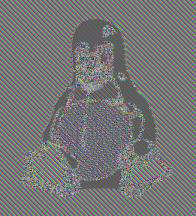
\includegraphics[width=\linewidth]{figures/TuxECB.png}
              \caption{\gls{ecb} encryption of the picture}
              \label{fig:tuxecb}
          \end{figure}
      \end{minipage}
  \end{minipage}

\subsubsection{\gls{cbc}}

This mode uses an \gls{iv} and can therefore be used for encryption of same messages without changing the key. Additionally, \gls{cbc} can also be used
for \gls{mac2} generation, as shown in section \ref{Integrity}.
\\
Encrypting a message is shown in Figure \ref{fig:cbc_encrypt}.
\begin{center}
$ C_0 = E(k, (M_0 \bigoplus IV ) )  $
\\
$ C_1 = E(k, (M_1  \bigoplus C_0) ) $
\\
$...$
\\
$ C_i = E(k, (M_i \bigoplus C_{i-1} ) )  $
\end{center}
To reverse the process, i.e. decrypt the message, see Figure \ref{fig:cbc_encrypt}
\begin{center}
$ M_0 = D(k, C_0) \bigoplus IV $
\\
$ M_1 = D(k, C_1) \bigoplus C_0 $
\\
$...$
\\
$ M_i = D(k, C_i) \bigoplus C_{i-1} $
\end{center}
The \gls{iv} does not have to be kept private, but must be known to the receiver of the message. It is important that such an \gls{iv} is unpredictable, otherwise
allowing a \gls{cpa}. Also, it must not repeat over the lifetime of the key, otherwise introducing the \gls{ecb} problem again. 
\\
The \gls{iv} introduces overhead, which is more problematic for  shorter messages.
To avoid such a message expansion, a solution is to use a "nonce", which stands for "\textit{n}umber used \textit{once}", as suggested in \cite{cryptoEng}.
Sender and receiver must maintain a message counter. This message counter must be encrypted to avoid predictability, and can then be used as \gls{iv}. Care must
be taken for the counter not to overflow within the lifetime of a key.

\begin{figure}
    \centering
    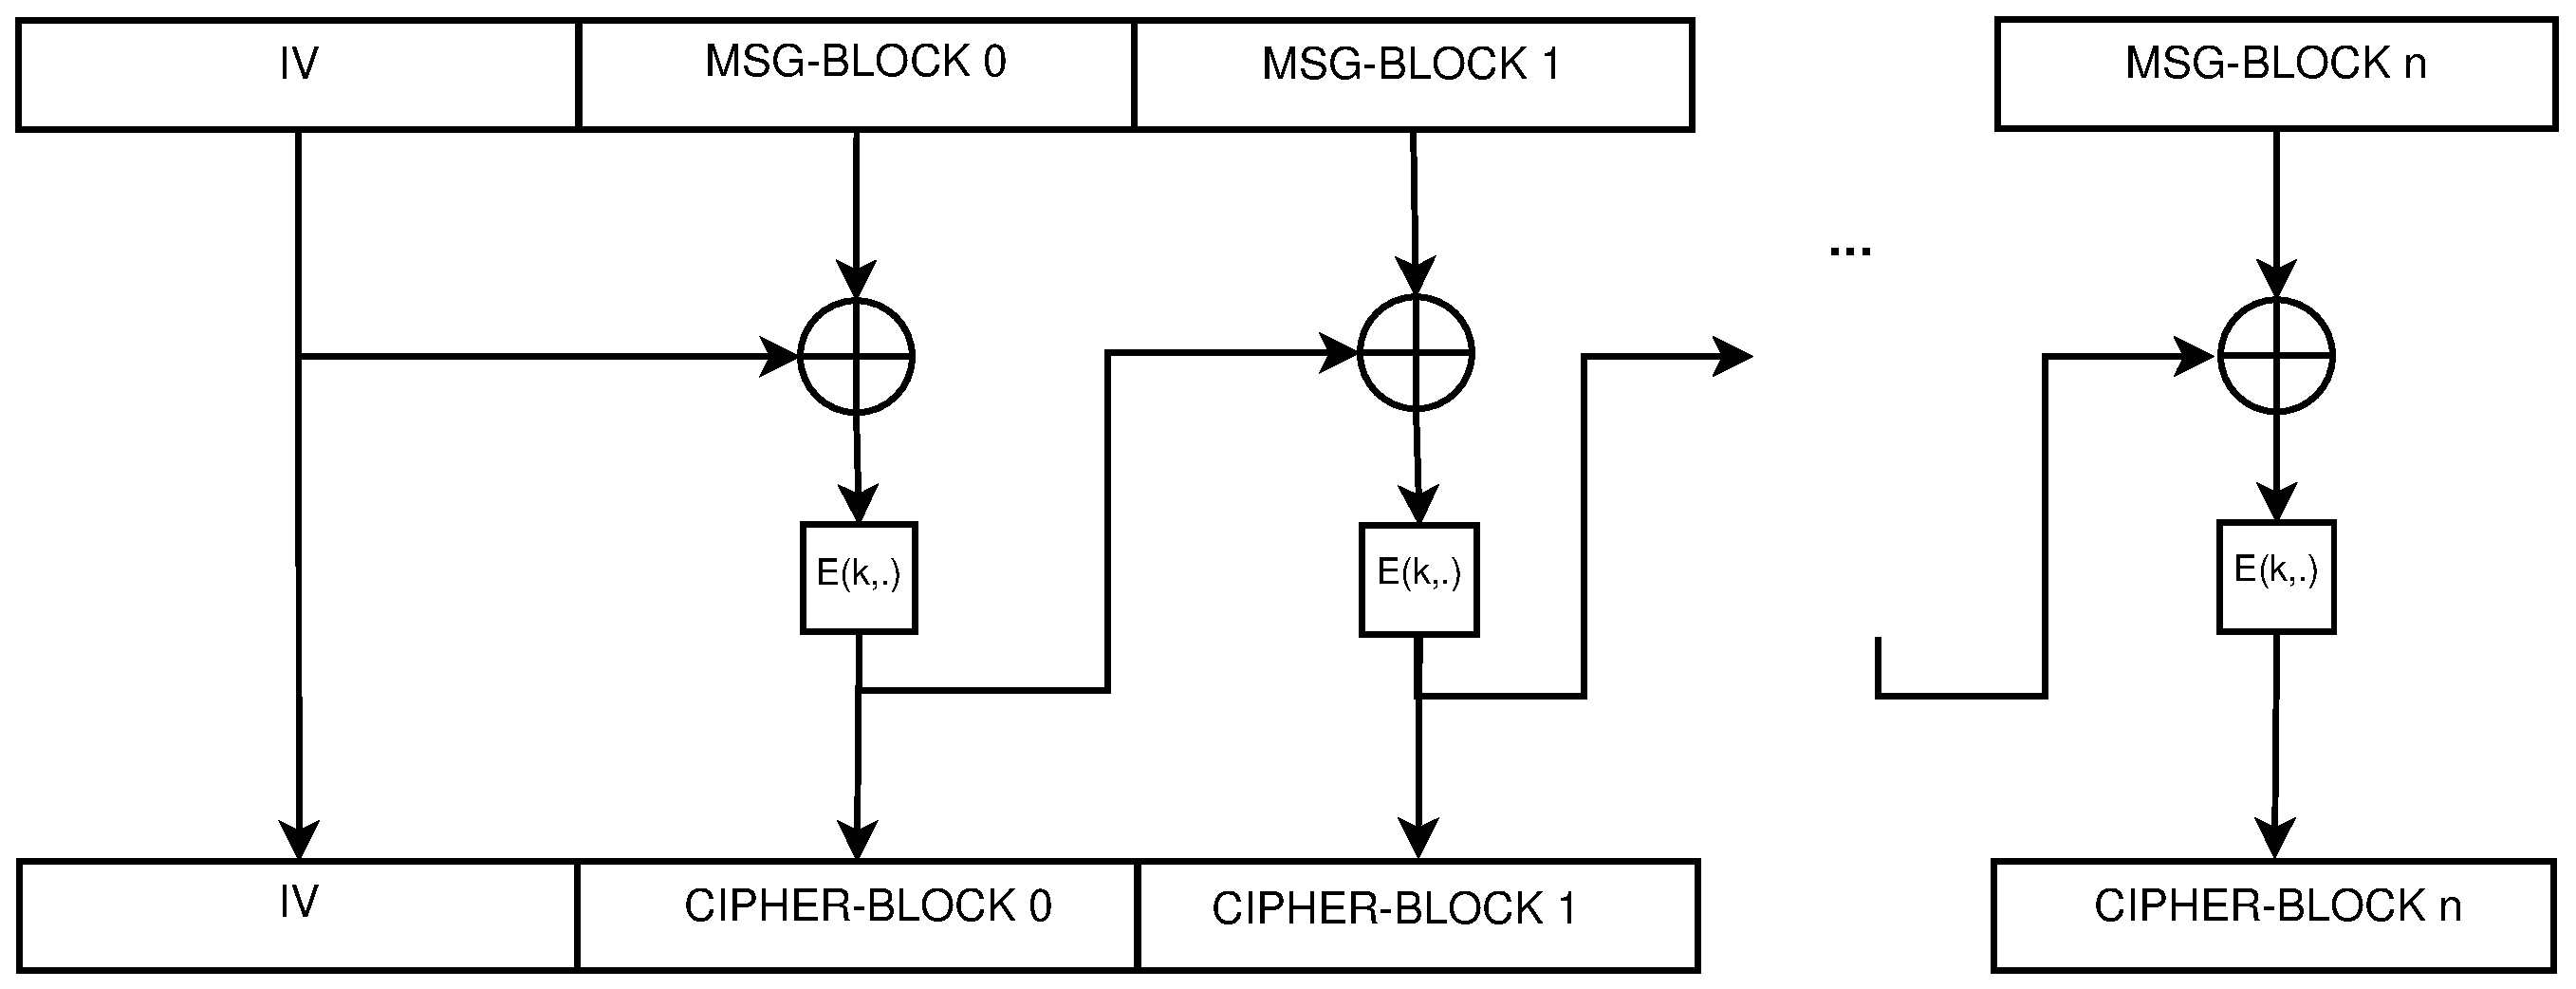
\includegraphics[width=1\textwidth]{figures/CBCencrypt.eps}
    \caption{\gls{cbc} for encrypting messages}
    \label{fig:cbc_encrypt}
\end{figure}

\begin{figure}
    \centering
    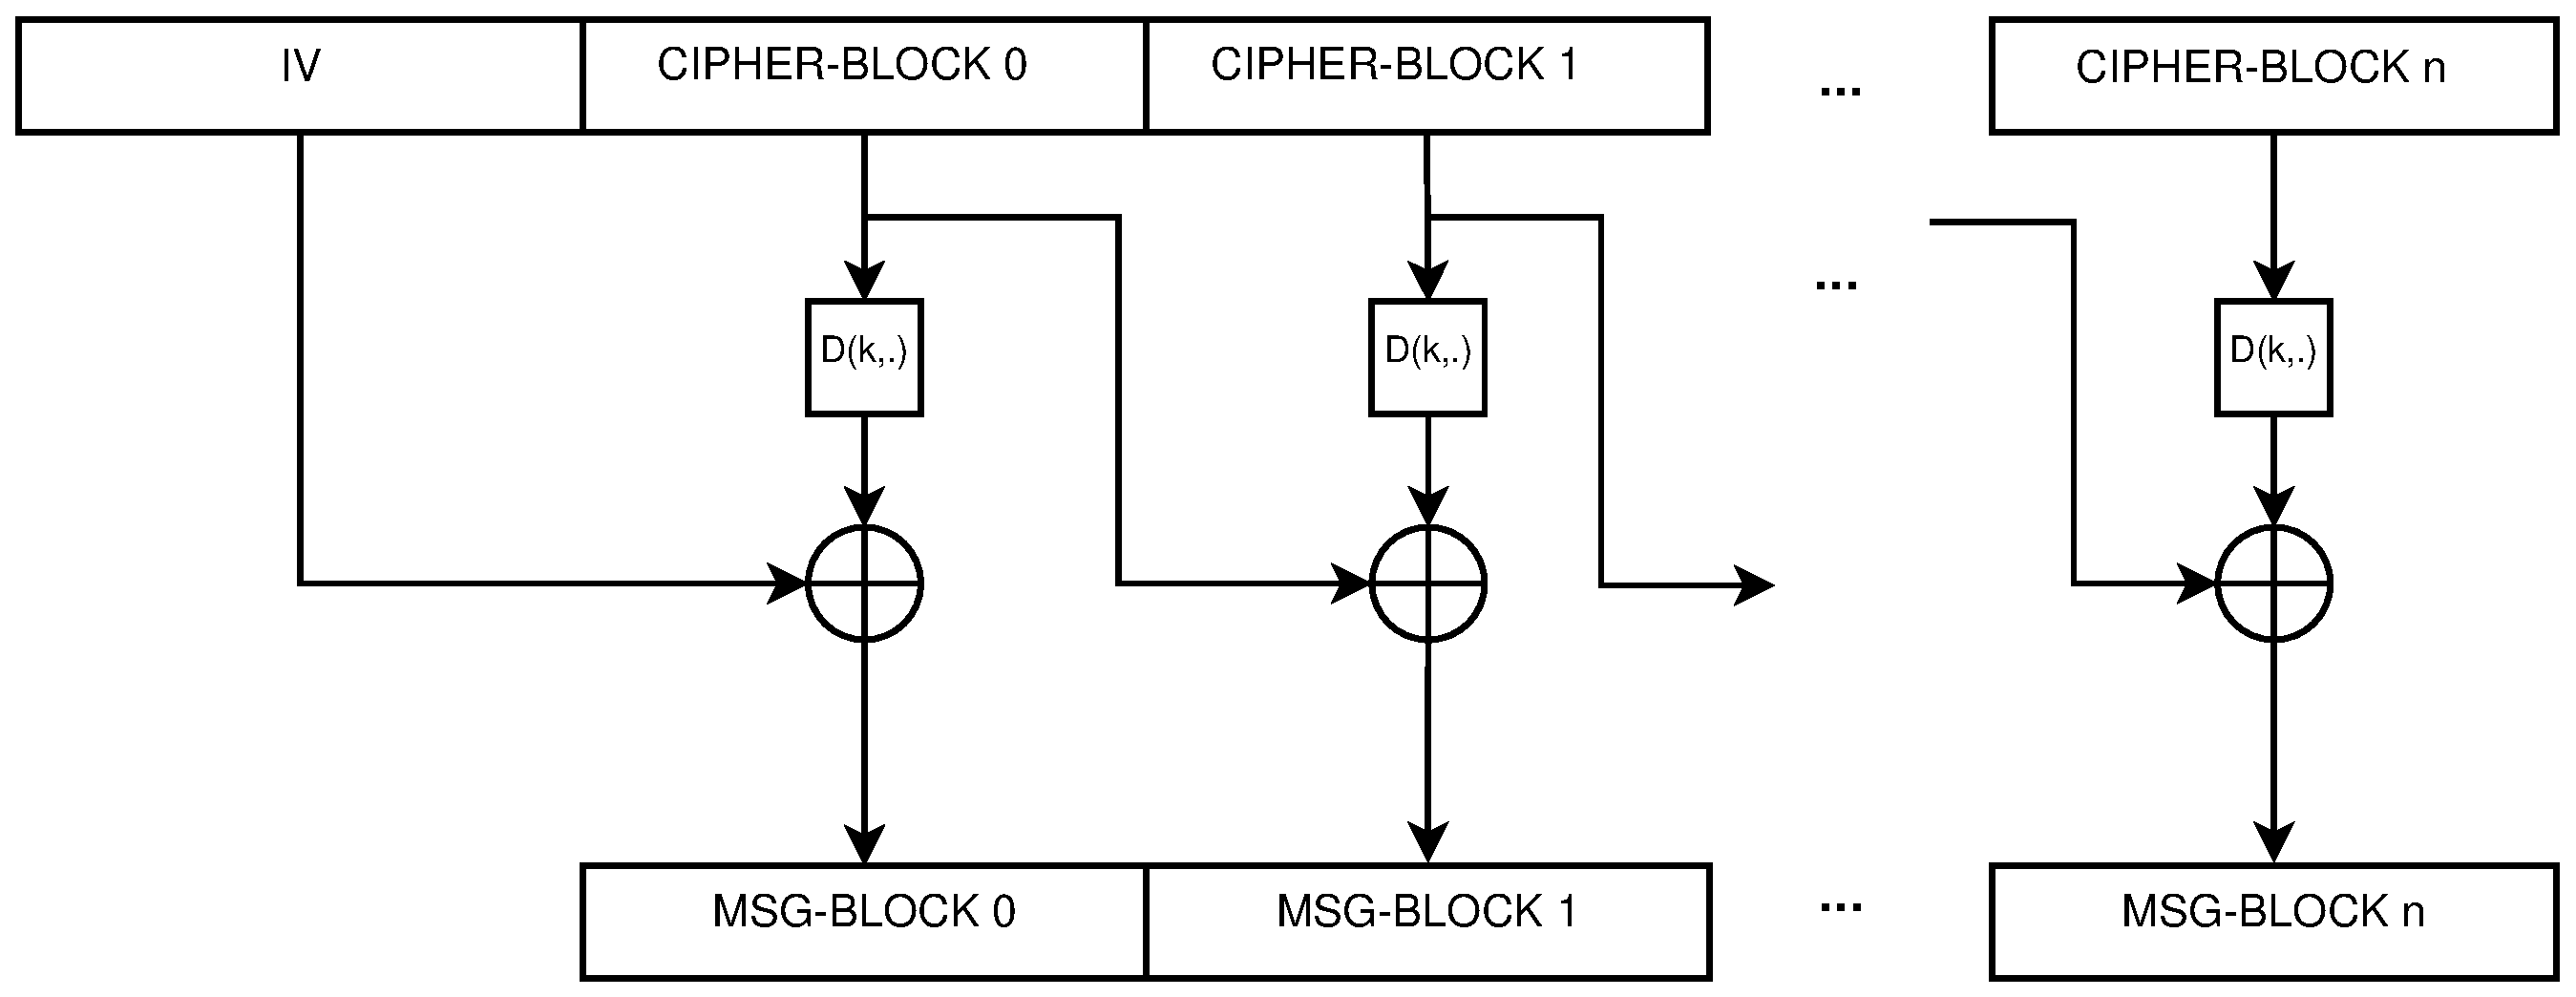
\includegraphics[width=1\textwidth]{figures/CBCdecrypt.eps}
    \caption{\gls{cbc} for decrypting messages}
    \label{fig:cbc_decrypt}
\end{figure}

\subsubsection{\gls{ctr} mode}

This confidentiality mode generates a key stream by encrypting a counter value with a block cipher. The key stream is then applied to the cleartext
blocks with the \gls{xor} operation, as shown in Figure \ref{fig:ctr}. For the last block, the key stream is truncated to match the size of the cleartext block.
\\
Decryption works by generating the same key stream on the receiver's side, and applying the \gls{xor} operation to the ciphertext blocks, similar to the
decryption process used in the Vernam cipher.
\begin{figure}
    \centering
    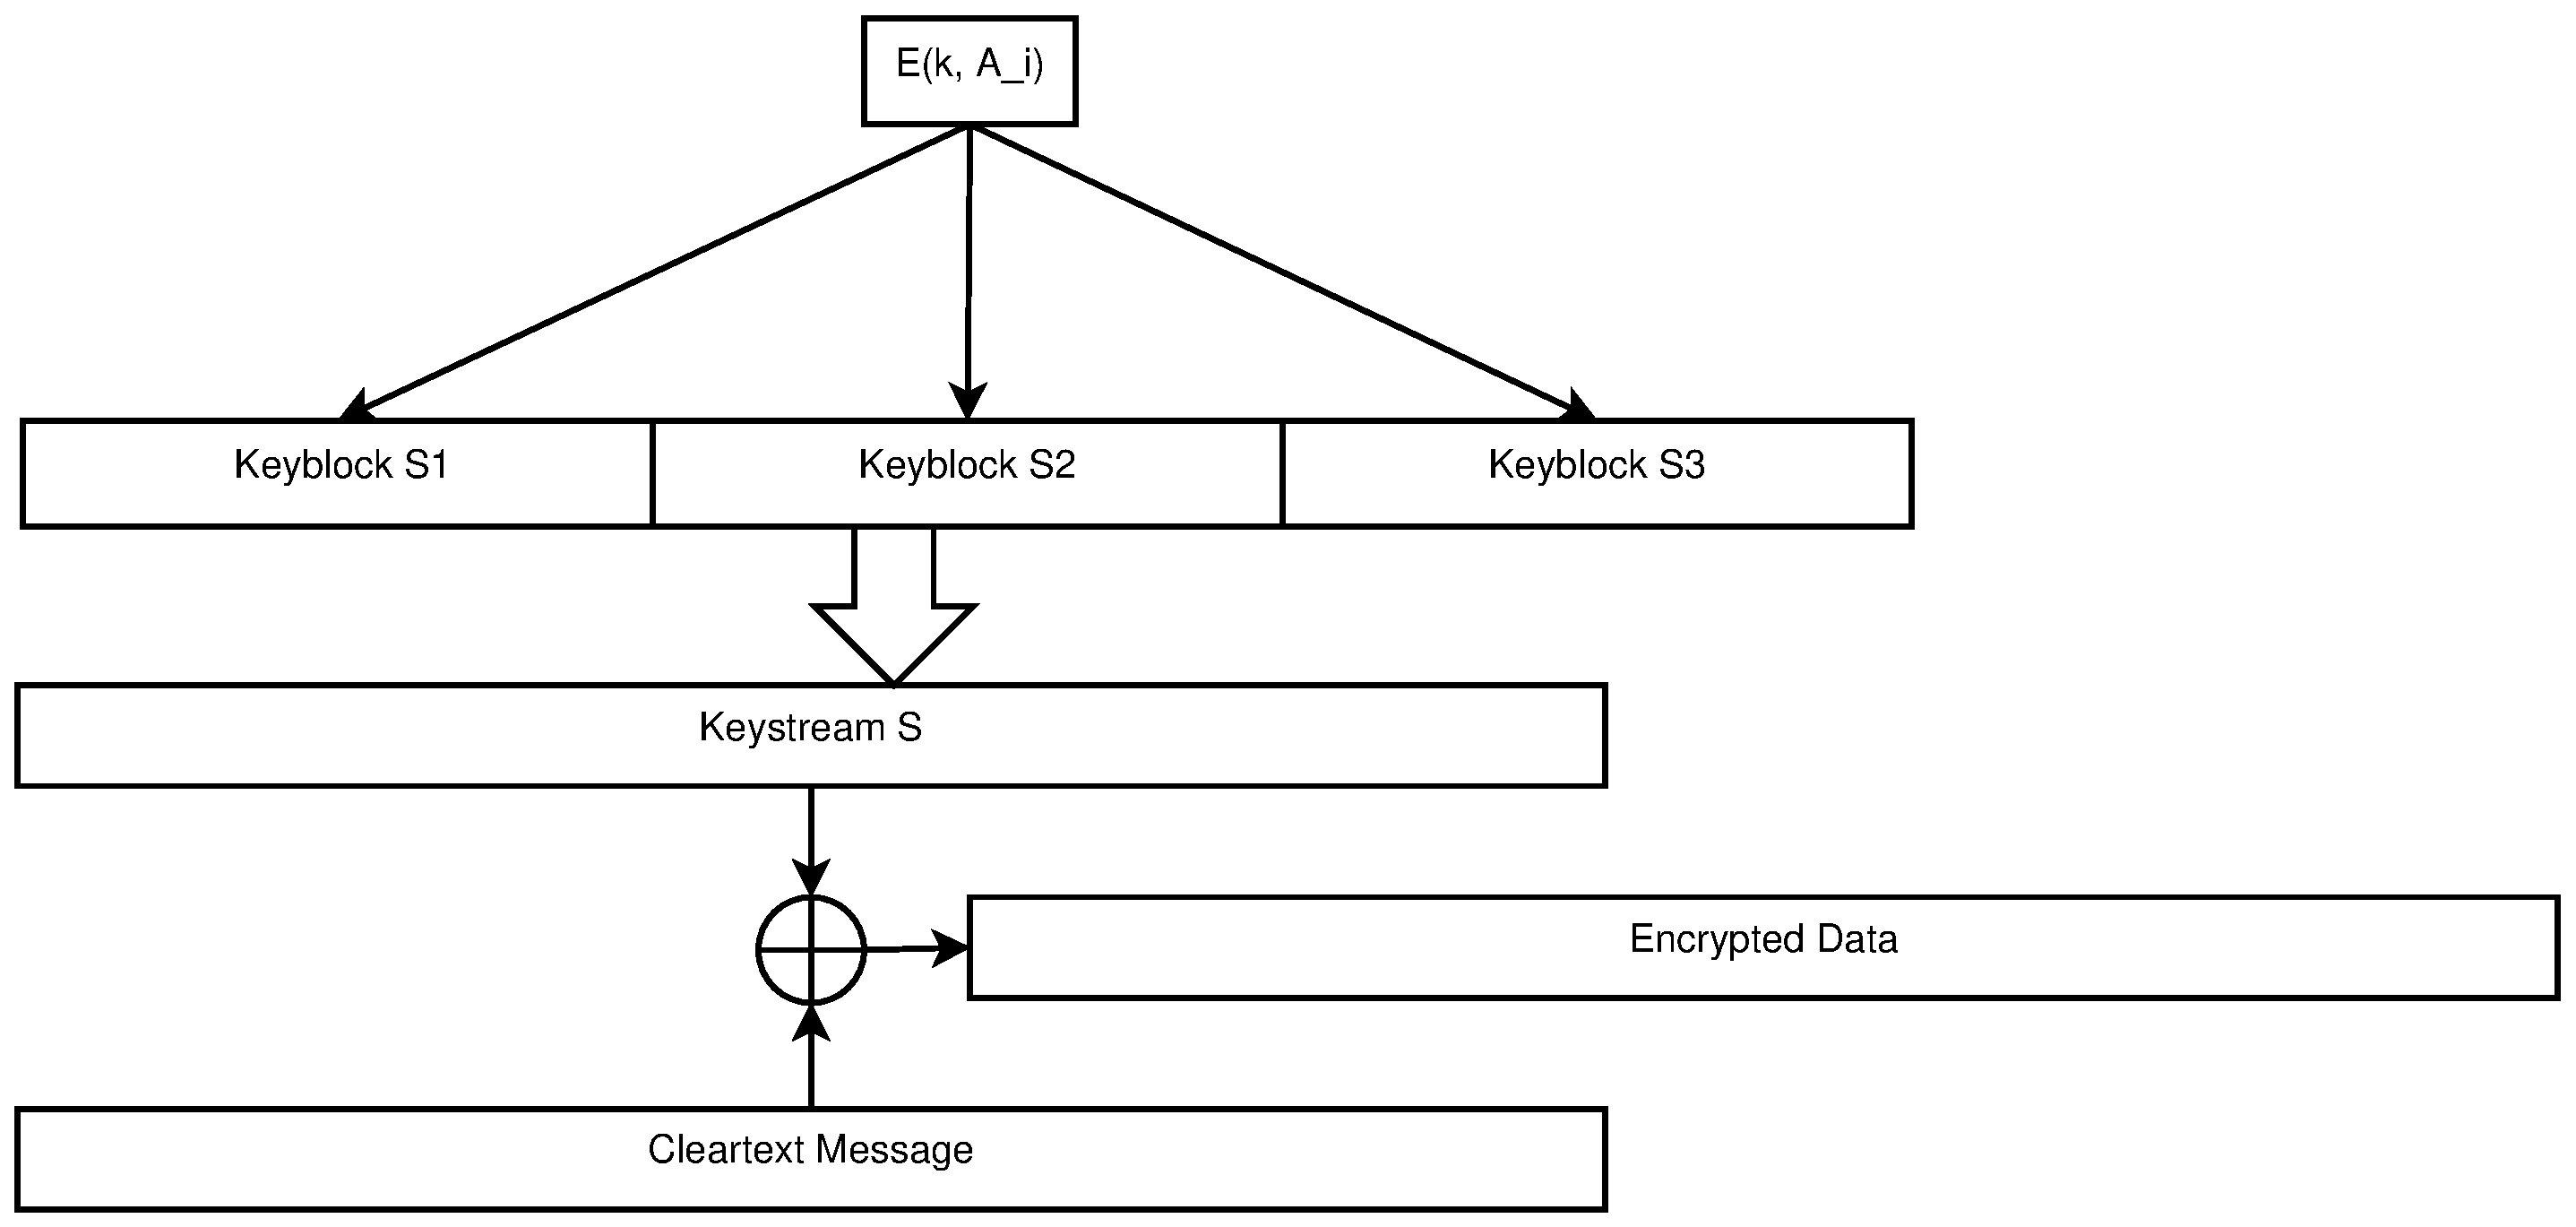
\includegraphics[width=0.8\textwidth]{figures/CTR.eps}
    \caption{\gls{ctr} mode encryption}
    \label{fig:ctr}
\end{figure}
To avoid the duplicate usage of the same counter value in bidirectional communication, the counter can be combined with a sender-dependent nonce by
concatenation before encrypting the counter:
\begin{center}
 $K_{0} = E(k, nonce || Ctr_0)$\\
 $K_{1} = E(k, nonce || Ctr_1)$\\
 ...\\
 $K_{i} = E(k, nonce || Ctr_i)$\\
 $C_i = K_i \bigoplus M_i$
\end{center}
 
\subsubsection{\gls{cfb}}
\gls{cfb} can be used to turn a block cipher into a stream cipher. Beside the block size $b$, another parameter $s$ determines the operation. $s$ corresponds
to the size of one transmission unit. For initialization, an unpredictable \gls{iv} is set as input for the underlying block cipher. Then, in every
processing step a new transmission unit is generated by \gls{xor}ing the $s$ most significant bits
of the output of the encryption function with the $s$ bit message unit. After that, the \gls{iv} is shifted to the left and the gap is filled
by the newly generated character, as shown in Figure \ref{fig:cfb}:
\\
\\
 $C[0] = E(k, IV[0:b-1])[b-1:b-s-1] \bigoplus M[0]$\\
 $C[1] = E(k, IV[0:b-s-1] || C[0])[b-1:b-s-1] \bigoplus M[1]$\\
 ... \\
 $C[n] = E(k, IV[0:b-ns-1] || C[0] || C[1] || .. || C[n-1])[b-1:b-s-1] \bigoplus M[n-1]$\\
\\

To decrypt, the same encryption function, \gls{iv} and key is used to retrieve one transmission unit at a time.
 
\begin{figure}
    \centering
    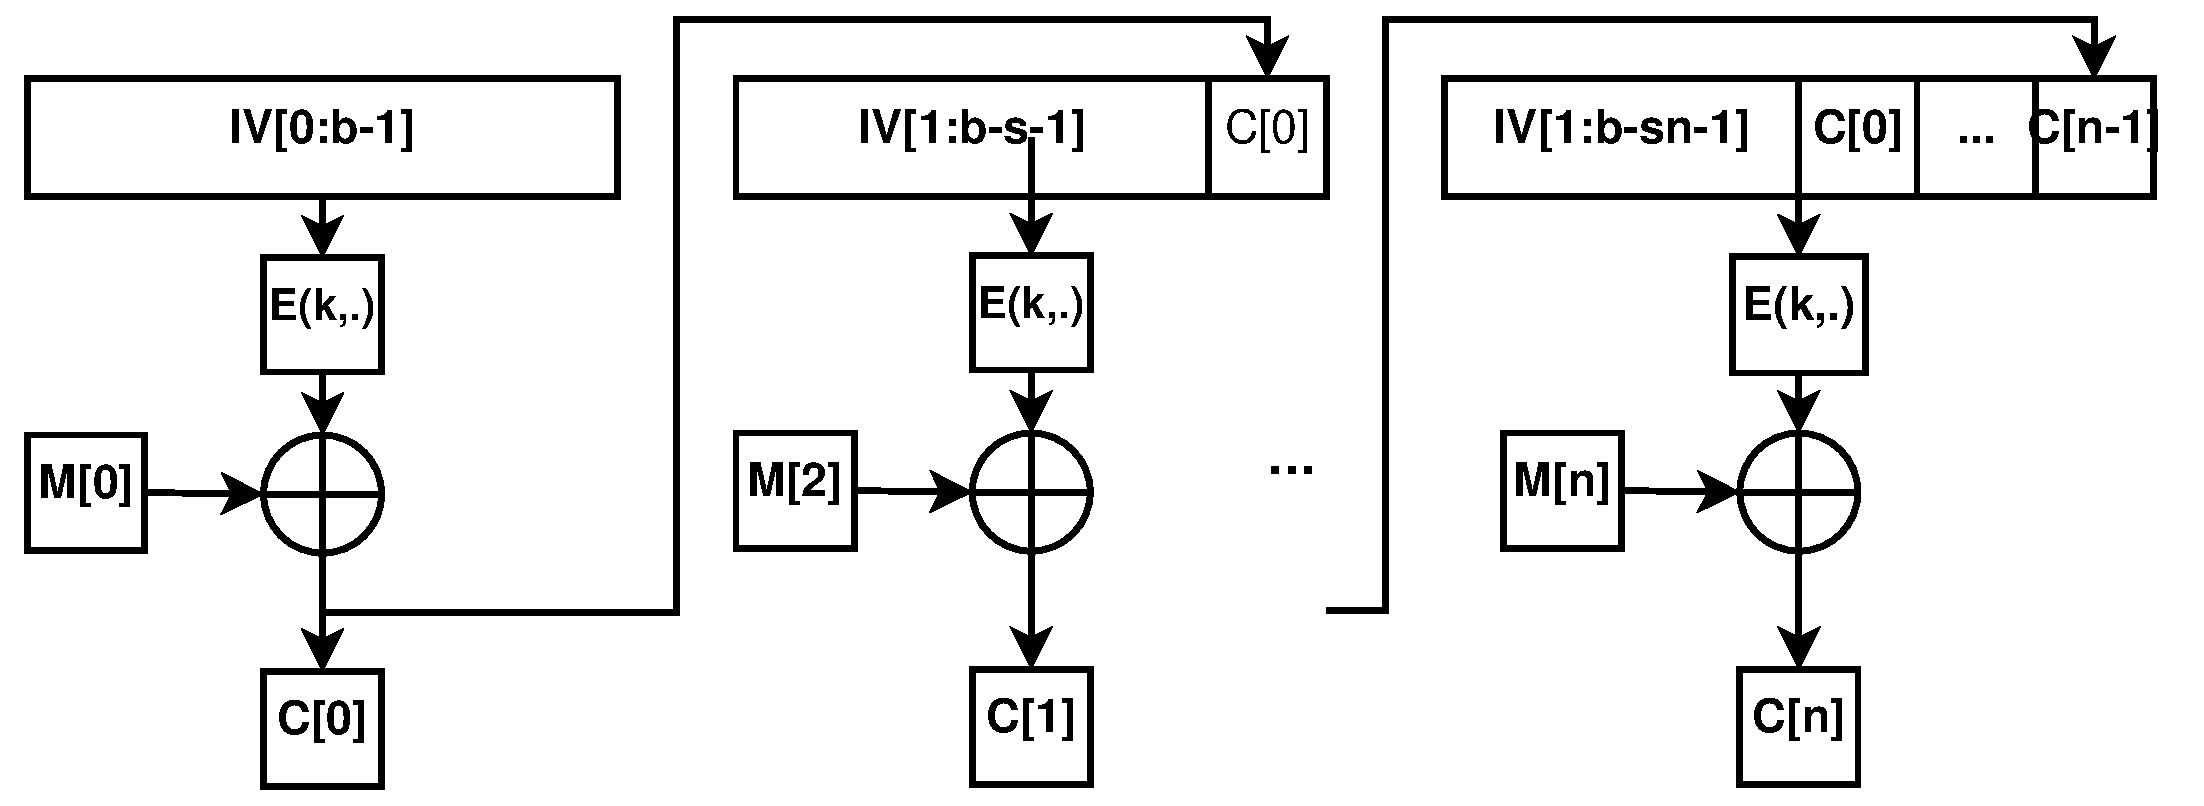
\includegraphics[width=1\textwidth]{figures/CFB.eps}
    \caption{CFB Encryption}
    \label{fig:cfb}
\end{figure}

\subsubsection{\gls{ofb}}
This mode is very similar to \gls{cfb}, but here the $s$ bit output from the encryption function is used directly to update the space caused by the \gls{iv} 
left shift. This avoids error propagation in case a transmission unit was damaged on transmit and thus a bit changed its value:
for \gls{ofb} encryption systems, one or more bit errors in one ciphertext character only affects the decryption of this character. In contrast, one bit error in \gls{cfb} affects
decryption of all following characters.
\\
\\
$O_0 = E(k, IV[0:b-1])[0:s-1]$\\
$C[0] = O_0 \bigoplus M[0]$\\
 $O_1 = E(k, IV[0:b-1] || O_0)[0:s-1]$\\
 $C[1] = O_1 \bigoplus M[1]$\\
 ... \\
 \\
 $0_n = E(k, IV[0:ns-1] || O_0 || O_1 || O_{n-1})[0:s-1]$\\
 $C[n] = O_n \bigoplus M[n]$\\

\begin{figure}
    \centering
    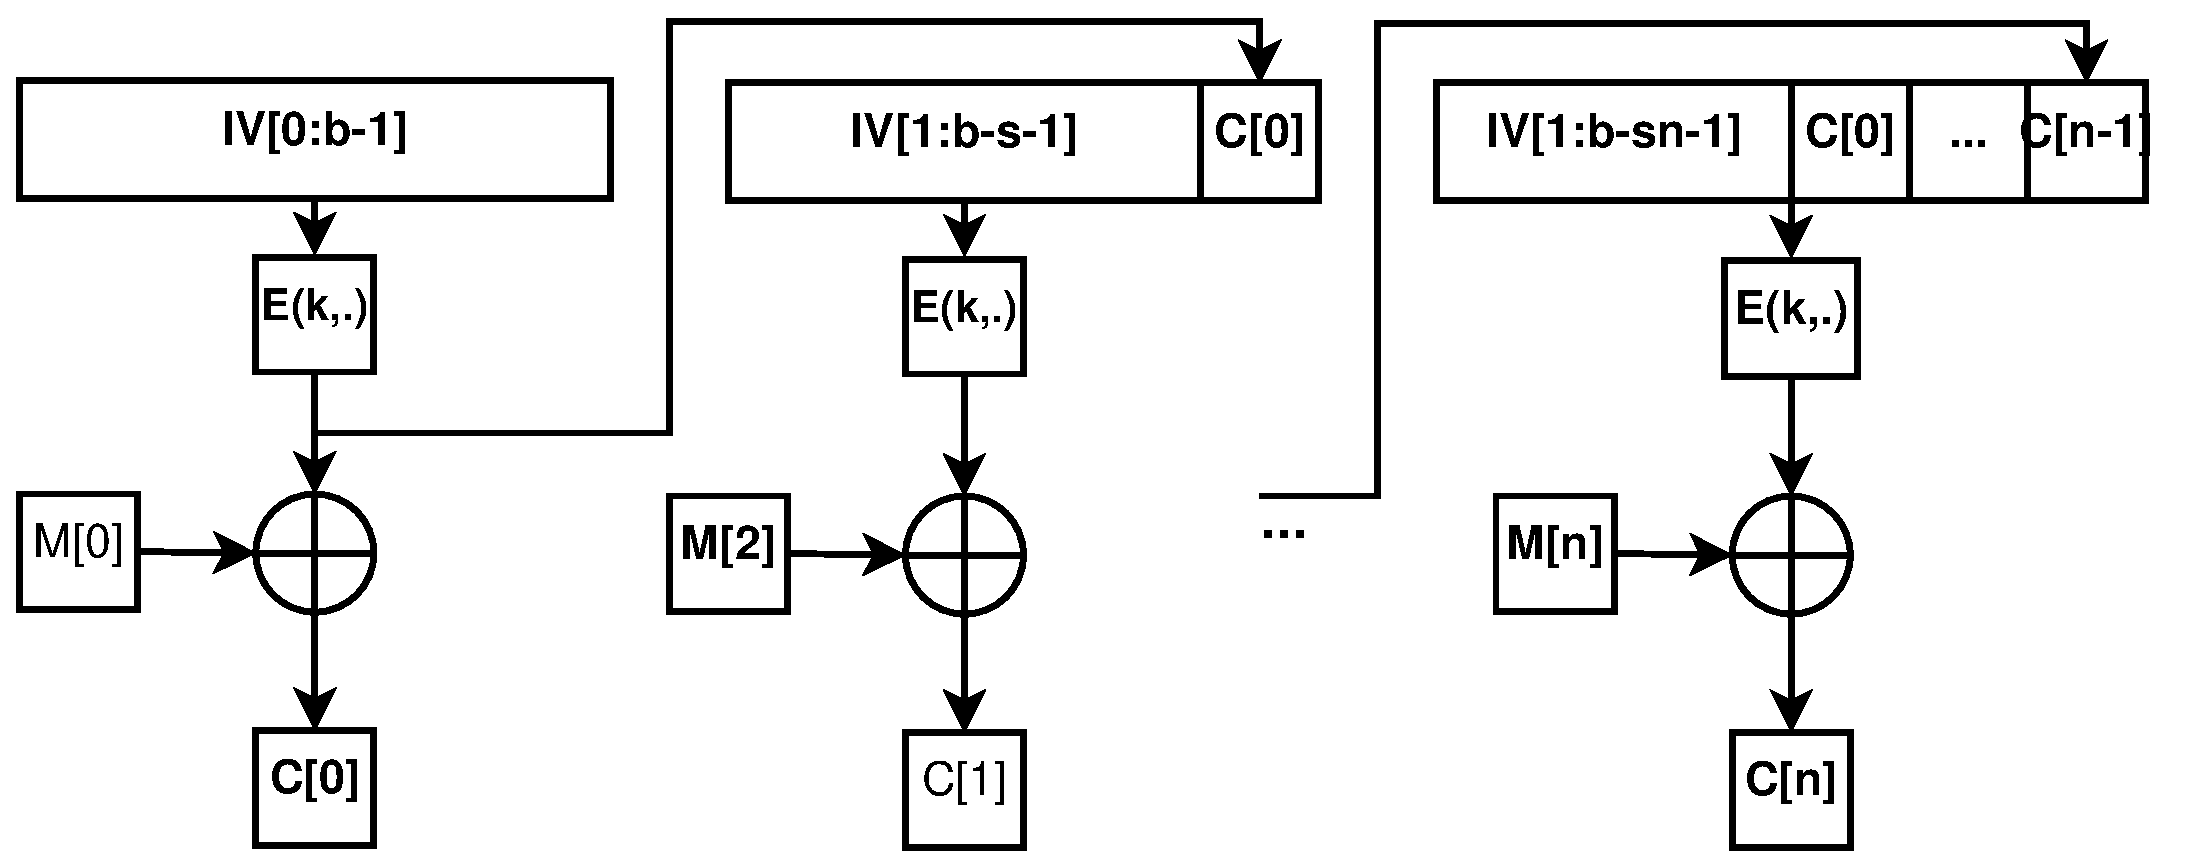
\includegraphics[width=1\textwidth]{figures/OFB.eps}
    \caption{OFB Encryption}
    \label{fig:ofb}
\end{figure}

\subsubsection{Integrity}\label{Integrity}
All modes of operation introduced so far are used to provide confidentiality only. To provide the second column of information security, i.e. integrity, in general
\glspl{mac2} or digital signatures are used.
Digital signatures are based on public key cryptography and are introduced in section \ref{digitalSignatures}. In contrast, \glspl{mac2} use symmetric keys,
providing integrity and authenticity. 
\\
The basic way to protect a data unit - be it a message traveling from sender to recipient or a file saved for later usage - from modification by a third party is to
generate a tag $t$, also called \gls{mac2}, and concatenating this tag to the message, as shown in Figure \ref{fig:tag}.
Verifying the integrity is done by re-generating the tag and comparing it to the saved one. 
\\
\\
In contrast to confidentiality modes, which should always be combined with a method to guarantee integrity, 
integrity-only modes do have a right to exist. For example, archives containing source code for open source project, available from the internet, must not be
encrypted but should be secured against modification. For example, the UNIX based operating system "FreeBSD" uses asymmetric keys to protect its package
management system from adversary modification.
\\
\\
Combining integrity and confidentiality in a security scheme called \gls{ae} will be handled in section \ref{authEncrypt}.
\\
\\
As tag generation and tag verification algorithms, keyed or unkeyed cryptographic secure hash functions are used.
For integrity-only, keyed hash functions must be used, or
otherwise an arbitrary entity can modify the message undetectable by regenerating the correct tag. Therefore, a simple checksum like a \gls{crc} or an unkeyed 
hash function can not provide integrity only, simply because the function value can be re-generated by an adversary modifying the message, allowing to mount
an attack called \gls{mac2} forgery.
Nevertheless, in combination with a confidentiality mode such an unkeyed function \textit{may} be secure, although its use is discouraged because many applications operating
this way are broken and can be attacked (i.e. \gls{ssh} version 1 \cite{zalewskissh}).
\\
\\
A hash functions takes as input an arbitrary large message $\mathcal{M}$ and generates a hash value $t = h(\mathcal{M})$ of fixed size, therefore $|M| >> |t|$. This many-to-one
mapping implies the existence of collisions, i.e. the existence of distinct messages $m_1, m_2$ which are mapped to the same tag $t$.
\begin{figure}
    \centering
    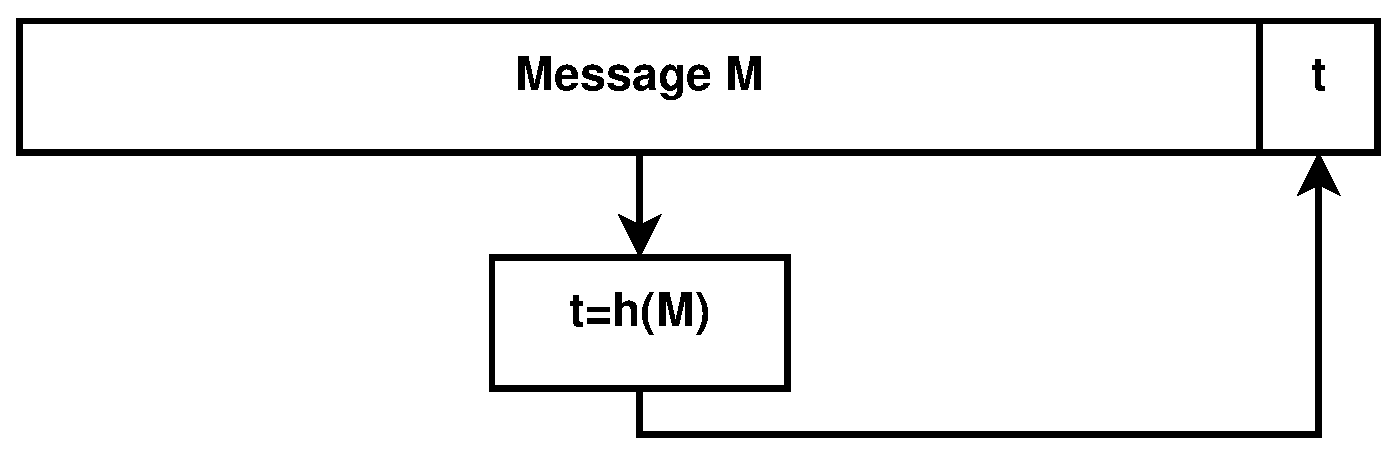
\includegraphics[width=0.8\textwidth]{figures/tag.eps}
    \caption{Tag generation}
    \label{fig:tag}
\end{figure}
\\
\\
To be cryptographically secure, a hash function must fulfill specific properties \cite{6732428}: firstly, while it should be easy to generate the tag
by calculating $t = h(m)$, reversing the process to get $m$ by executing $h(t)^{-1}$ should be hard, a property called \textit{preimage resistance}. 
Additionally, \textit{2nd-preimage resistance} assures that for any given message $m$ and corresponding tag $t$, it must be infeasible to find a second message
that maps to the same tag. Finally, \textit{(strong) collision resistance} states that it also must be infeasible to find any two messages generating
the same tag, therefore collision resistance implies 2nd-preimage resistance \cite{handbookCR}.
\\
\\
Important representatives of cryptographically secure hash functions are the family of \glspl{sha}, with variants providing hashes of 160, 256, 384 or 512 bit 
length, defined by \gls{nist} \cite{nistSHA}. For \gls{sha}-1, an attack to find collisions was found \cite{Wang05findingcollisions} and should therefor not
be used anymore.
\\
Because these hash functions lack a secret key and therefore would allow \gls{mac2} forgery, a construction called \gls{hmac} can be used, which takes 
additionally to the message $m$ as input a key $k$, and $ipad$ and $opad$ being constant values \cite{hmac}.

\begin{align}
 t = S(k, m) = h((k \bigoplus opad) || h((k \bigoplus ipad) || m)) 
\end{align}
\\
\\
A different way for tag-generation, called \gls{cbc}-\gls{mac2}, is based on block ciphers, utilizing a construction similar to \gls{cbc} mode encryption,
shown in Figure \ref{fig:cbc_MAC}. 

\begin{figure}\label{cbcMAC}
    \centering
    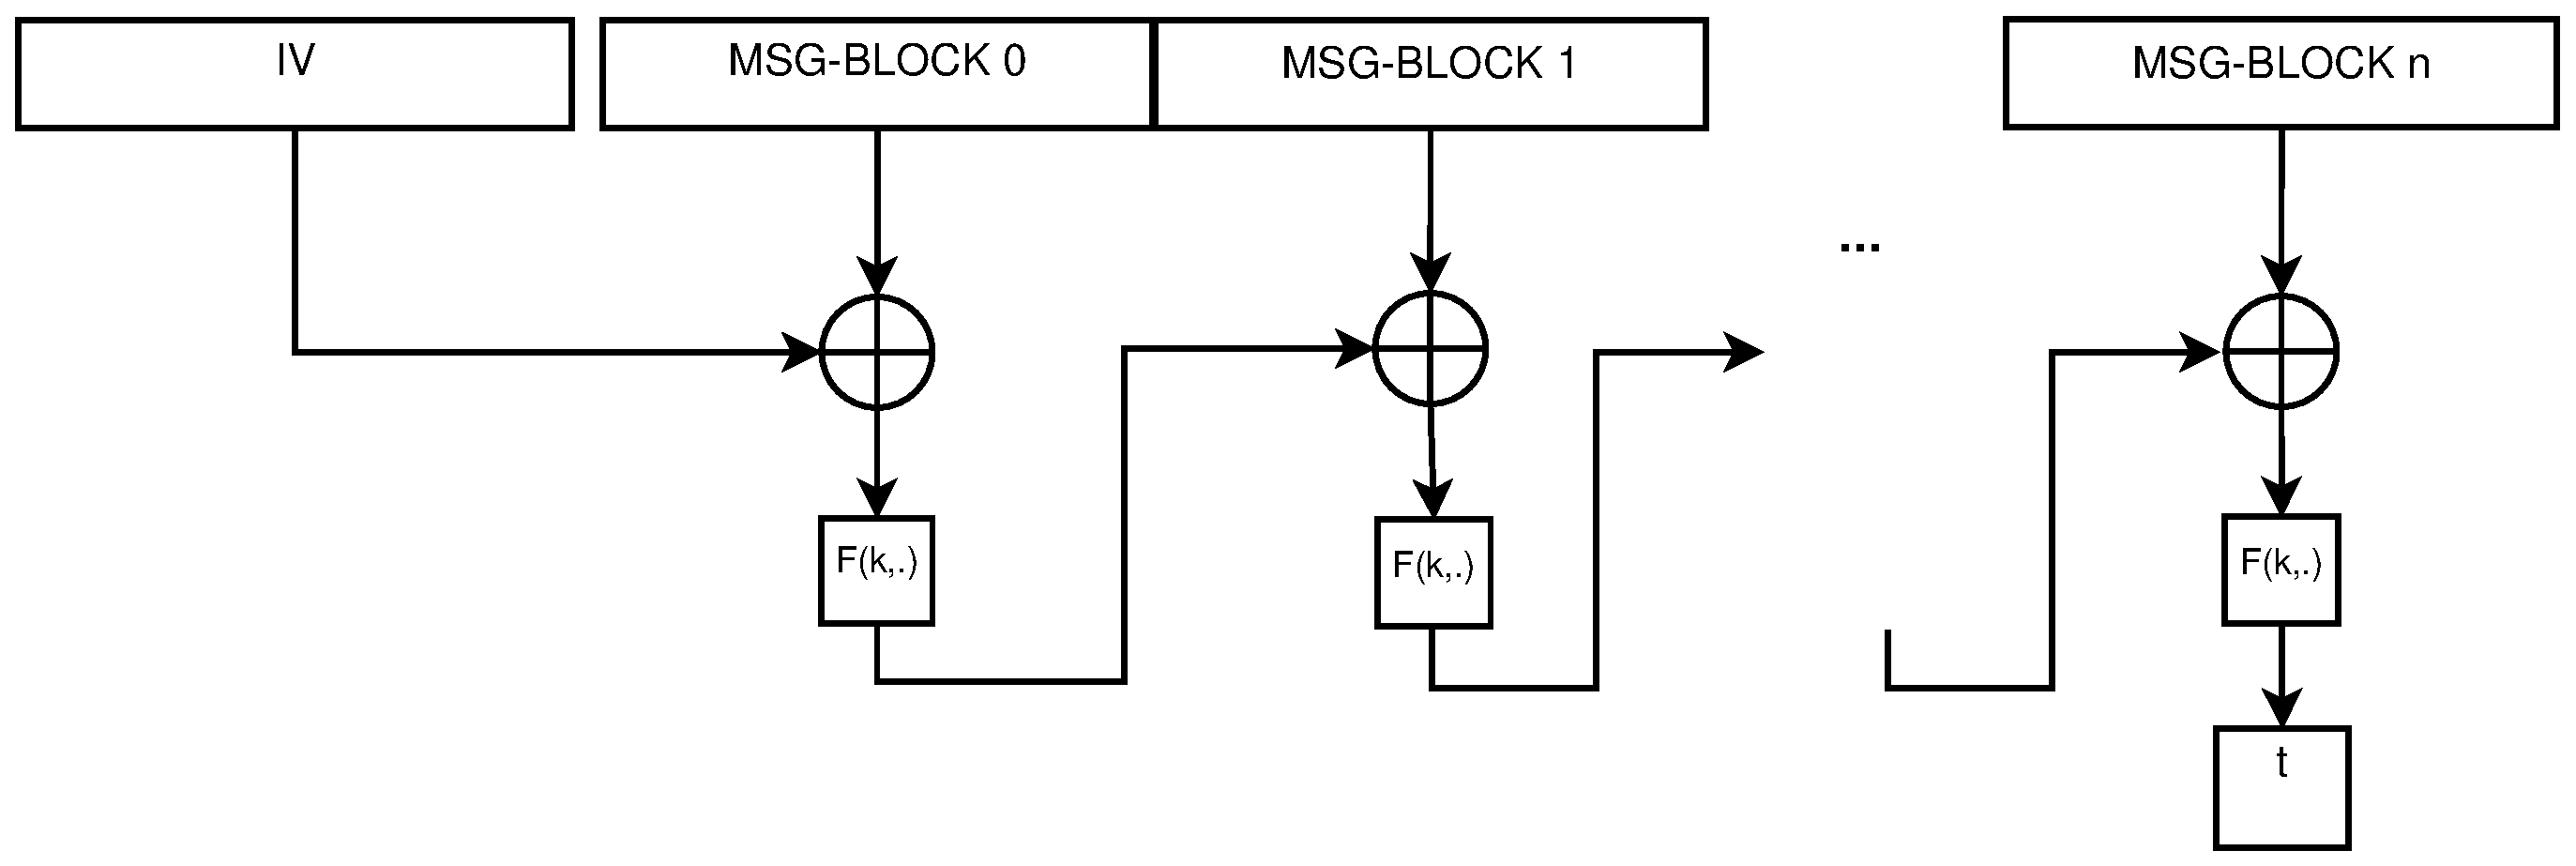
\includegraphics[width=1\textwidth]{figures/CBCMac.eps}
    \caption{\gls{cbc} for generating a MAC}
    \label{fig:cbc_MAC}
\end{figure}

\begin{figure}\label{cbcMACFlags}
    \centering
    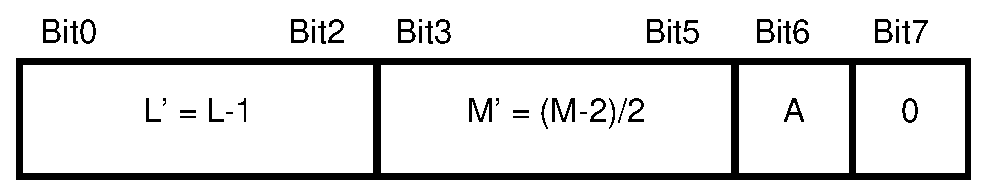
\includegraphics[width=0.8\textwidth]{figures/CBCIVFlags.eps}
    \caption{Flag Field of CBC IV}
    \label{fig:cbc_Flags}
\end{figure}

\section{Authenticated Encryption}\label{authEncrypt}

Many applications demand the integration of confidentiality \textit{and} integrity modes. The need for confidentiality is self explaining in systems where
submitted data must be protected from a passive adversary. One example would be a password for logging into a remote computer, sent over a network connection
- just by monitoring the connection, an attacker can steal the password and gain illegitimate access to the system.
\\
\\
The need to additionally provide integrity and authenticity measurements is maybe not that obvious, but can be motivated in various ways. For example, two entities
sharing an initial key known to both of them which want to negotiate a temporary session key could randomly choose the temporary key, encrypt it and send it
to the other side. Even if a passive adversary knows that the package he monitors will be used as session key he cannot derive it, provided a secure cipher is
used.  In contrast, an active attacker can intercept and modify the encrypted session key, and afterwards inject the modified message. The receiver
would then decrypt the package, thus obtaining a modified session key. After all, the two entities would use two different keeps, crippling their communication.
\\
\\
To avoid that attacks, methods to provide encryption and integrity are combined. Basically, 3 different ways how this can be achieved exist:
\begin{itemize}
 \item "encrypt-and-mac" encrypts the message $m$ and appends the tag $t$ of the cleartext message
 \begin{align}\label{encAndMac}
  c = E(k_e, m) || h(k_h, m)
 \end{align}
 \item "mac-then-encrypt" generates the tag for the cleartext message $m$, appends it and afterwards encrypts cleartext + tag to get ciphertext $c$:
 \begin{align}\label{macThenEnc}
  c = E(k_e, m || h(k_h, m))
 \end{align}
 \item "encrypt-then-mac" encrypts the message $m$ first, and afterwards appends the tag $t$ of the encrypted message to obtain $c$
 \begin{align}\label{encThenMac}
  c = E(k_e, m) || h(k_h, E(k_e, m))
 \end{align}
\end{itemize}
For all 3 schemes, $E(k, m)$ must be a semantically secure encryption function, and $h(k, m)$ denotes a keyed, cryptographically secure hash function.
The latter is of particular importance for \ref{encAndMac}, because this scheme otherwise directly leaks information about the plaintext in the tag. 
\\
As general, cryptographic data should always be authenticated first. Only if authenticity can be verified,
the encrypted data should be processed further.
Following this rule, it turns out that only \ref{encThenMac} is considered generically secure against chosen plaintext attacks.
"Encrypt-and-mac" \cite{sshBellare}, used in \gls{ssh}, is considered generically
insecure. For "mac-then-encrypt", used in \gls{ssl}, the same holds true, but this scheme can be used in a secure manner if \gls{cbc} or a stream cipher like 
\gls{ctr} mode is used for encryption.

\subsection{CCM}

\gls{ccm} \footnote{http://tools.ietf.org/html/rfc3610}, combines \gls{cbc} for authentication and \gls{ctr} for encryption.
\gls{ccm} generates the \gls{mac2} for the message first, appends this \gls{mac2} to the cleartext data and afterwards encrypts data and \gls{mac2} with counter mode, thus using a
\textit{MAC-then-Encrypt} scheme. The only supported block size is 128-bit blocks, so it is possible, but not mandatory, to use 128-bit \gls{aes} as underlying block cipher.
\\
Two application dependent parameters have to be fixed first: 
\begin{itemize}
 \item M: Number of octets in the \gls{mac2} field. A shorter \gls{mac2} obviously means less overhead, but it also makes it easier for an adversary to guess the correct
 value of a \gls{mac}, so valid values are $M \in \{4, 6, 8, 10, 12, 14, 16\}$. 
 \item L: Number of octets in the length field. This is a trade-off between the maximum message size and the size of the nonce. Valid values are $2 \leq L \leq 18$.
 For example, when setting $L = 2$, 2 bytes are reserved for the length field, which means that the biggest message that can be encrypted is of size 64kB. The actual
 length of the message is filled into the field named 'length(msg)', as shown in Figure \ref{fig:cbc_MAC}.
\end{itemize}
Both parameters are encoded in the very first byte of the first message block, thus reducing the possible maximum size of the nounce, as shown in Figure \ref{fig:cbc_Flags}.
Bit 6 of the length field is set to 1 if additional authenticated data are sent, and bit 7 is reserved and set to 0.


\subsubsection{Generating the \gls{mac2}}

As shown in Figure \ref{fig:cbc_MAC}, the first message block $M_0$ is \gls{xor}'d with a nonce or \gls{iv} (see Figure
\ref{fig:ccrMacIV}), which must be unique per key to avoid deterministic encryption.
The result of the \gls{xor} operation is then feed to the block-cipher to get the first cipherblock $C_0$. The encrypted data $C_0$ gets \gls{xor}'d with the next message block $M_1$, and this
result becomes the input for the block cipher, and so on, iterating over all $n$ message blocks to determine the tag $t$:

\begin{figure}
    \centering
    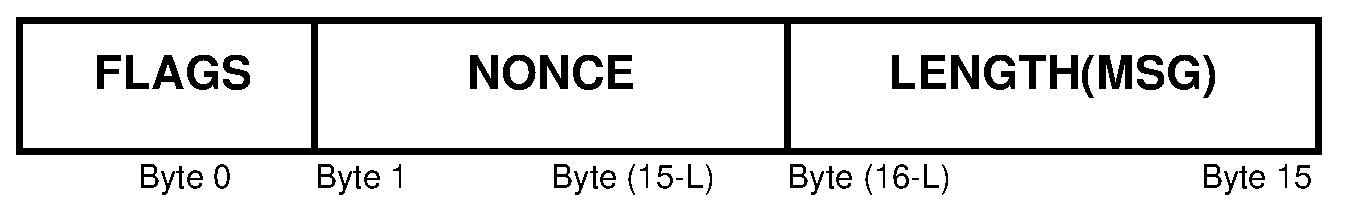
\includegraphics[width=0.8\textwidth]{figures/CCMCBCIV.eps}
    \caption{\gls{iv} for \gls{cbc} \gls{mac2}}
    \label{fig:ccrMacIV}
\end{figure}


\begin{center}
 $C_0 = F(k, M_0 \bigoplus IV )$
 \\
 $C_1 = F(k, M_1 \bigoplus C_1) $
 \\
 $...$
 \\
 $C_n = F(k, M_n \bigoplus C_{(n-1)})$
 \\
\end{center}

The resulting tag $t$ can be truncated, corresponding to the chosen \gls{mac2} size $M$:
\begin{center}
  $t = C_n[M:0]$, with $M \in \{4, 6, 8, 10, 12, 14, 16\}$
\end{center}
which means that the tag $t$ consists of the least significant $M$ bytes of the output of the last encryption block.

\subsubsection{Encrypting Data and \gls{mac2}}

\gls{ctr} is used for encrypting the actual payload and the concatenated, \gls{cbc} mode generated \gls{mac2}.
Thus, authenticated encryption is achieved in a manner also called 'mac-then-encrypt'. While authenticated
encryption modes implementing this ordering (generating the \gls{mac2} first, then encrypt data and \gls{mac2}) \textit{may}
be vulnerable to padding oracle attacks \cite{eurocryptVaudenay02}, \gls{ctr} effectively avoids these attacks simply because
there is no padding needed.
\\
\gls{ctr} implements a weaker form of the one time pad by generating a keystream of sufficient
length, and then applying the \gls{xor} operation to the keystream and the data, as shown in Figure \ref{fig:ctr}.
\\
\\
First, keyblocks with 16 byte length each are generated by encrypting the nounce, a flag and a counter with the key. These 
keyblocks are then concatenated and trimmed to the proper length (i.e., the length of the message to encrypt). This obtained keystream
is then bitwise \gls{xor}'ed with the cleartextmessage (which consists of the data and the MAC), yielding the final encryption.


\section{Public Key Cryptography}\label{pkc}

Public Key Cryptography solves the problem of establishing a secure channel by using an insecure one.
Here sender and recipient use two different keys: one for encryption, called \textit{public key}, the other
for decryption, called \textit{private key}. This key pair belongs together, hence this scheme is also called \textit{asymmetric} encryption. A fundamental requirement
is that it must be hard
to derive the decryption key from the encryption key. This behavior is achieved by some kind of public known one-way function where it is computationally
easy to calculate the result of $f(x) = y$, but only given $y$, it is computationally - in the domain of processing power and/or memory - hard
to reverse this function to get $x$.
The basic idea for such a one-way function was formulated for the first time in the year 1874 by William Stanley Jevons stating:
\\
\\
\textit{"Can the reader say what two numbers multiplied together will produce the number 8616460799? I think it unlikely that anyone but myself will
ever know."} \cite{wStanley} 
\\
\\
Although his statement was not related to cryptography at all, and of course factoring of much bigger numbers is doable nowadays, this statement exactly describes
the spirit of public key systems, and the security of RSA, introduced below, is directly connected to the inability to factor large numbers in reasonable time.
\\
Because disclosure of the public key does not affect the security of the scheme, the public key can be published in some sort of dictionary.
An entity wanting to send an encrypted message to a receiver can then look up the receiver's public key, encrypt the message and send the resulting
ciphertext to the recipient, who then can decrypt the message. 
\\
\\
It is remarkable that any algorithm establishing public keys must authenticate its participants, or it will be vulnerable to man-in-the-middle attacks.

\subsection{Merkle Puzzles}
In \cite{Merkle}, Ralph C. Merkle developed an algorithm for key exchange between two parties. While the algorithm is based on symmetric ciphers and is
not practicable, it motivates the usage of public key systems based on algebraic structures and is therefore introduced.
\\
\\
The key idea is that the necessary work by the two legitimate parties when negotiating a key is bounded by $O(n)$, while an adversary must spend $O(n^2)$ to 
also calculate the key, thus generating a quadratic gap. 
Merkle defines a puzzle as cipher text that is supposed to be broken. This can be achieved by restricting the size of the symmetric key used such that an
exhaustive search can be finished in feasible time. Every puzzle contains an id and a session key, both chosen randomly, as well as a static string,
known to all participants.
\\
The party initiating the key exchange, called $X$, generates $n$ such puzzles and sends all of them to the receiver $Y$. $Y$ picks one puzzle at random and
decrypts it by trying all possible keys. Because of the static string inside the puzzle, $Y$ knows for sure when the correct key has been tried.
$Y$ then extracts the session key and sends the corresponding id back to $X$. Subsequently, both parties can use the session key referenced by the id for encryption.
An eavesdropper $Z$, monitoring all puzzles, cannot directly determine which of them is containing the returned id and therefore does not know the session key the 
two parties agreed on - the only possibility for $Z$ is to attack \textbf{all} puzzles, squaring the effort spent by $X$ and $Y$.
\\
If, for example, one puzzle can be broken by $2^{32}$ computations, and $2^{32}$ different puzzles are used, $X$ must prepare, save and send $2^{32}$ puzzles
to $Y$, who in turn must try $2^{32}$ different keys. $Z$ must crack all $2^{32}$ puzzles, each with effort $2^{32}$, thus resulting in $2^{64}$ processing steps.
\\
While this algorithm is very wasteful in regards of processing power, memory and communication capacity, such a protocol would be useful if a more-than-quadratic
blowup could be achieved, but unfortunately, for all algorithms based on symmetric ciphers, this quadratic gap is the best that can be achieved,
as shown in \cite{Barak09merklepuzzles}.   
\\ 
To further increase the effort an attacker has to spend a different approach has to be found. It turns out that hard mathematical problems exist that are 
suitable for such a purpose. 
\\
Therefore, in the next sections three important public key algorithms are introduced: \gls{dh} key exchange, based on prime fields, \gls{ecc}, and RSA.
\subsection{\gls{dh} Key-Exchange}

Whitfield Diffie and Martin Hellman proposed a way to solve the problem for key-exchange based on finite fields
when they published their paper \textit{New Directions in Cryptography} in the year 1976 \cite{1055638}. The algorithm enables two entities to agree on a 
shared secret which never has to be transmitted between them. The security of their original algorithm
is based on the hardness of the \gls{dlp}, as shown in \ref{refDLP}.
\\
\\
With the original \gls{dh} algorithm, 2 entities - $A$ and $B$ - use exponentiation over finite fields to agree on a shared secret, which
then can be used parametrize a block or stream cipher. The first step for both entities is to agree on the set of parameters $\{p, g\}$, where $p$ is a 
large prime and $g$ is a generator of the cyclic group ${Z_p}^*$. These parameters are not secret and
can thus be sent over an unsecured channel.
Additionally, each entity randomly chooses an integer $x$ from the interval $(1, q-2]$, and calculates the value $y = g^x \pmod p$. $x$ is the private key,
$y$, which is computationally easy to calculate, is the public key. $A$ sends its public key $y_A \equiv g^{x_A} \pmod p$ to $B$, and $B$ its public key
$y_B \equiv g^{x_B} \pmod p$ to $A$. Due to the characteristics of exponentiation, $A$ and $B$ can now easily derive the shared secret by using its counterpart's
public key and raising it to the power of its own private key in the domain of ${Z_p}^*$:

\begin{center}
 $k_B \equiv {y_A}^{x_B} \equiv (g^{x_A})^{x_B} \equiv g^{x_A*x_B} \pmod p $\\
 $ = $ \\
 $ k_A \equiv {y_B}^{x_A} \equiv g(^{x_B})^{x_A} \equiv g^{x_B*x_A} \pmod p $
\end{center}
An eavesdropper that intercepts the initially sent parameter set $\{p, g, q\}$ and the public keys $y_A$ and $y_B$ and that wants to calculate the shared secret
$k_A = K_B$  must therefore calculate the discrete logarithm of $y_A$ or $y_B$ to the base $p$, i.e. must solve the \gls{dlp}, a hard problem as shown in
section \ref{refDLP}.
\\

%FIXME el gamal??
\subsection{\gls{ecc}}

The \gls{dh} protocol can be based on different kinds of cyclic groups. Koblitz and Miller independently proposed the usage of cyclic groups based on
\glspl{ec} \cite{eccKoblitz} \cite{eccMiller}. See \ref{pkc} for the theoretical introduction.
This cyclic groups are receiving increased importance in cryptography because they allow the usage
of shorter keys compared to \gls{dh} over prime fields or RSA, while providing the same level of secrecy.
\\
To build a public key system, two users $A$ and $B$ initially agree on a set of public \textit{domain parameters}. The most important parameters are \cite{ecDP}	
\begin{itemize}
 \item the order of the field, $q$
 \item the coefficients $a, b \in \mathcal{F}_p$, defining the \gls{ec}
 \item the coordinates $(x_p, y_p \in \mathcal{F}_p)$ of the \textit{base point} $P$, 
 \item the order of $P$, denoted $n$
\end{itemize}
After agreeing on this set, $A$ selects a randomly chosen integer $k_A$, calculates $P_A = k_A*P$ and sends
this point to $B$, who in turn randomly chooses $k_B$ and sends $P_B = k_B*P$ to $A$. Subsequently, both can calculate the point $k_A*k_B*P$, which can be used
to derive a key.

\subsection{Multi-party key negotiation}
\gls{dh} and therefore also the \gls{ecdlp} can be generalized to $n$ parties, obtaining one key in common. The key negotiation procedure for 3 parties, using
classical \gls{dh}, is
shown in Figures \ref{fig:dh1} and \ref{fig:dh2}, where it is assumed that all 3 parties $A$, $B$ and $C$ already agreed upon $(p,g)$.
\begin{figure}
    \centering
    \begin{tikzpicture}[scale=0.2]
\tikzstyle{every node}+=[inner sep=2pt]
\tikzstyle{arrow}=[draw, -latex] 
\tikzset{
    pil/.style={
           ->,
           thick,
           shorten <=1pt,
           shorten >=1pt,}
}

\usetikzlibrary{automata,positioning}
\usetikzlibrary{positioning}

\node[state,text width=1.5cm,align=center]	at (0,0)	(a)	{A}; 
\node[state,text width=1.5cm,align=center]	at (15,20)	(b)	{B}; 
\node[state,text width=1.5cm,align=center]	at (30,0)	(c)	{C}; 
\path[pil,->] (a)  edge[]   node[text width=3cm,align=left] {send $g^a$} (b); 
\path[pil,->] (b)  edge[]   node[text width=3cm,align=right] {send $g^b$} (c); 
\path[pil,->] (c)  edge[]   node[text width=1cm,align=center] {send $g^a$} (a); 
\end{tikzpicture}
   % 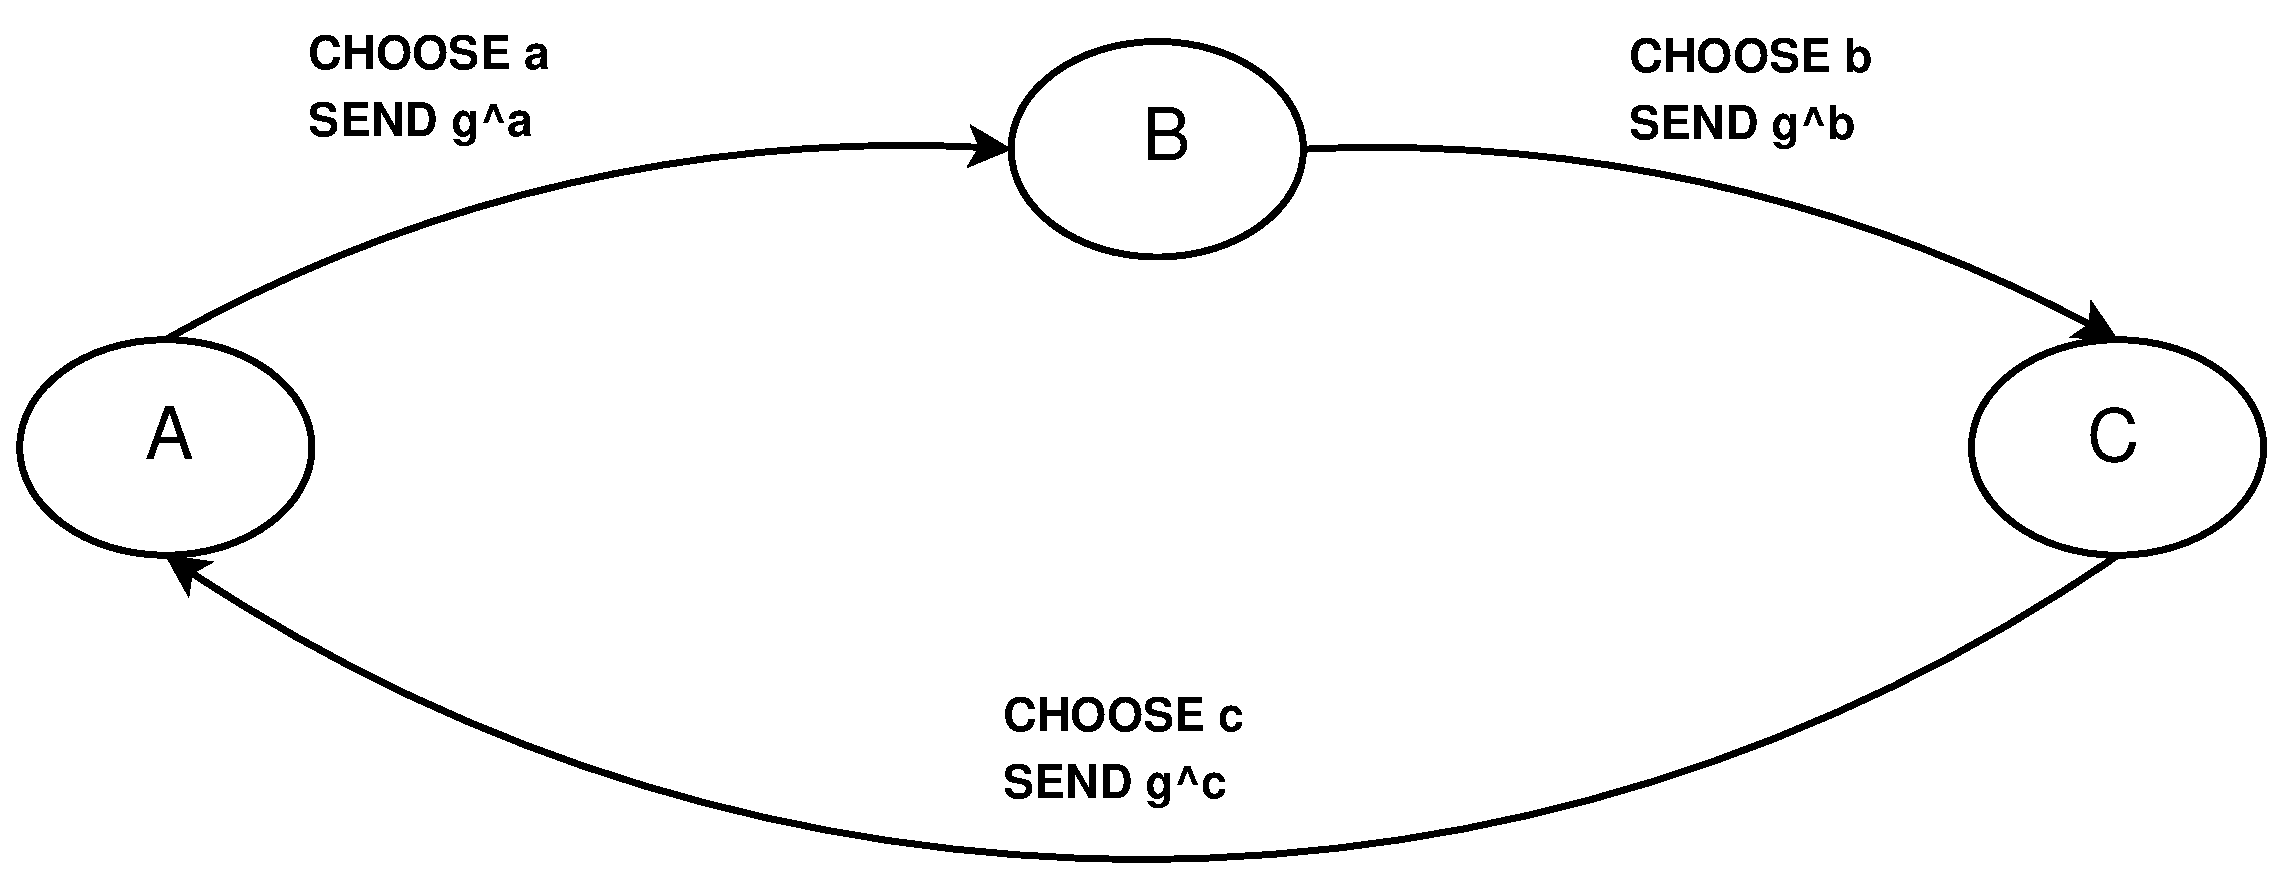
\includegraphics[width=0.8\textwidth]{figures/dh-group_round1.eps}
    \caption{\gls{dh} Round 1}
    \label{fig:dh1}
\end{figure}
\begin{figure}
    \centering
    \begin{tikzpicture}[scale=0.2]
\tikzstyle{every node}+=[inner sep=2pt]
\tikzstyle{arrow}=[draw, -latex] 
\tikzset{
    pil/.style={
           ->,
           thick,
           shorten <=1pt,
           shorten >=1pt,}
}

\usetikzlibrary{automata,positioning}
\usetikzlibrary{positioning}

\node[state,text width=1.5cm,align=center]					at (0,0)			(a)		{A}; 
\node[state,text width=1.5cm,align=center]				at (15,20)		(b)		{B}; 
\node[state,text width=1.5cm,align=center]					at (30,0)			(c)		{C}; 

\path[pil,->] (a)  edge[]   node[text width=4cm,align=left] {send $(g^c)^a$} (b); 
\path[pil,->] (b)  edge[]   node[text width=4cm,align=right] {send $(g^a)^b$} (c); 
\path[pil,->] (c)  edge[]   node[text width=1cm,align=center] {send $(g^b)^c$} (a); 

\end{tikzpicture}
   % 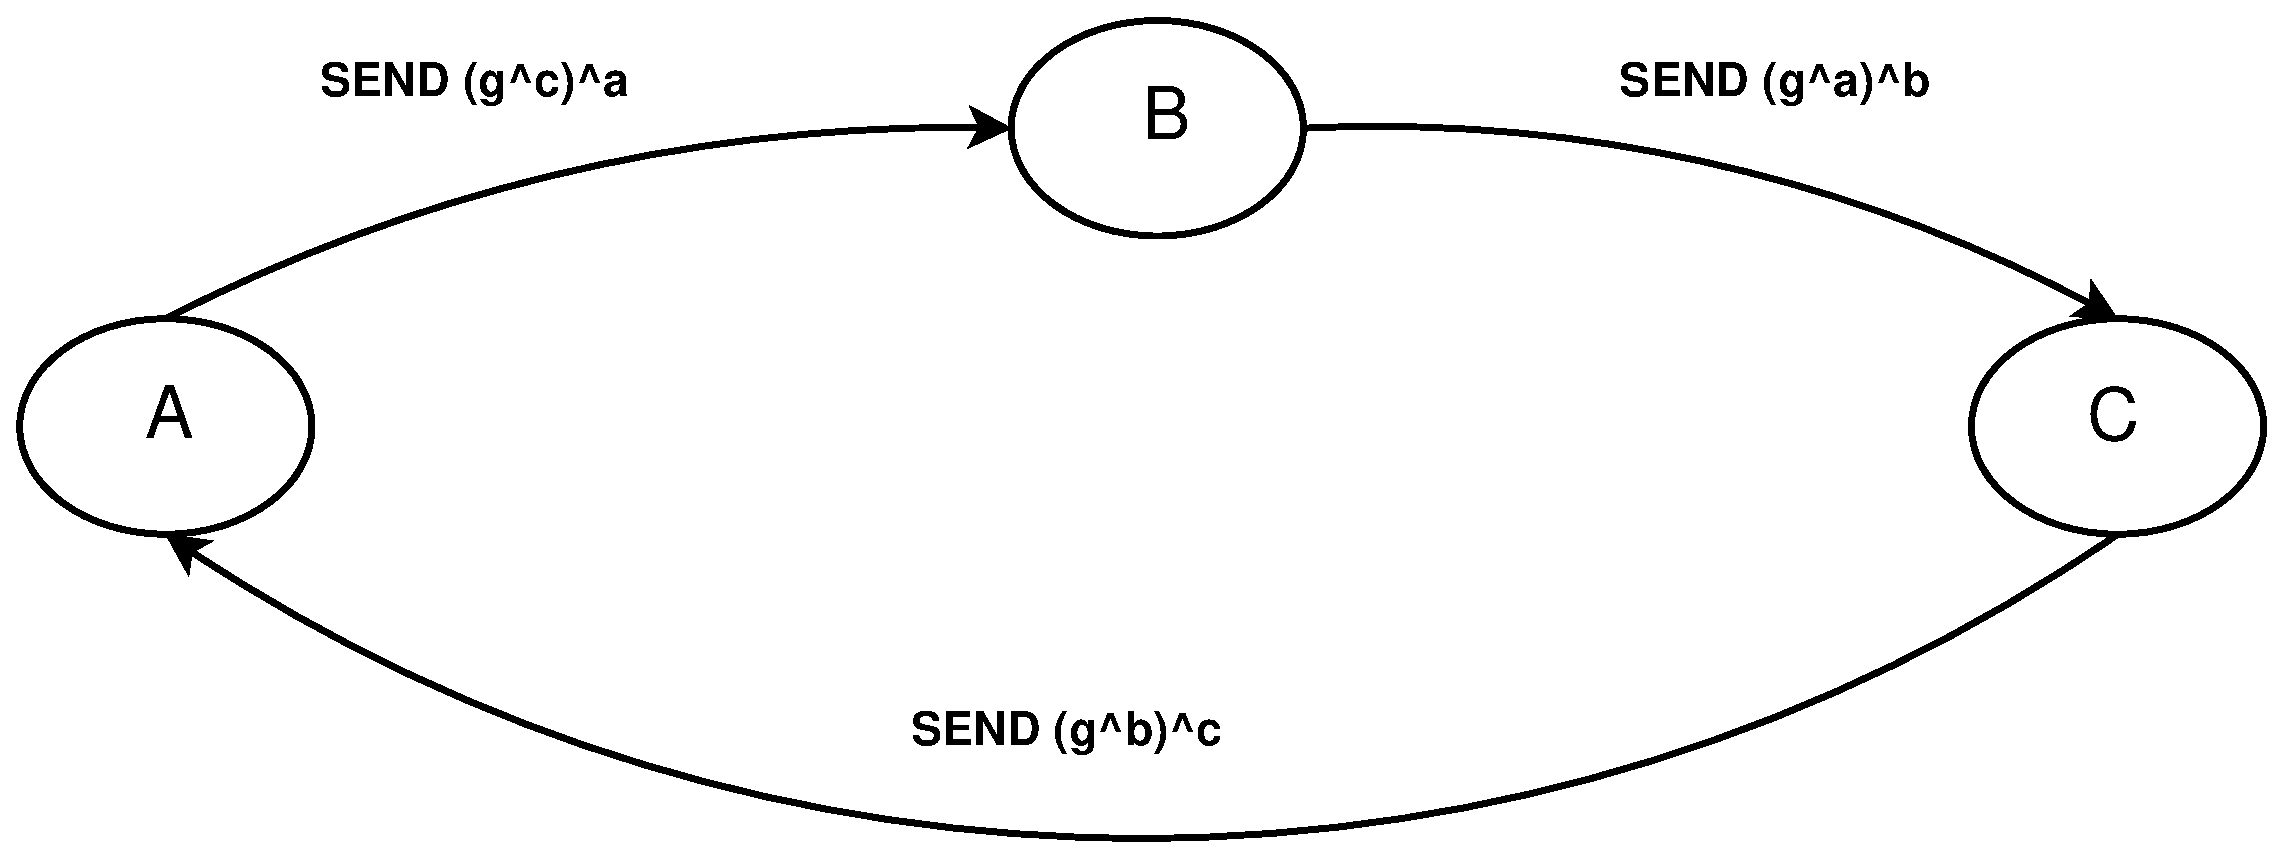
\includegraphics[width=0.8\textwidth]{figures/dh-group_round2.eps}
  \caption{\gls{dh} Round 2}
    \label{fig:dh2}
\end{figure}
After finishing the second communication round, every party raises the last received value to its own private key and thus derives the shared secret.
\begin{align}
 ((g^b)^c)^a = ((g^c)^a)^b = ((g^a)^b)^c = g^{a*b*c}
\end{align}
This algorithm can be generalized to $n$ parties, using $(n-1)$ communication rounds. Obviously, this algorithm may not be practicable for a large $n$. Additionally,
a complete new run must be executed whenever a new node joins.
\\
Additionally, this key agreement mechanism (as well as all others presented so far) uses no authentication and is therefore vulnerable to active attacks.

\subsection{RSA}

RSA, published in 1977 by Ron Rivest, Adi Shamir, and Leonard Adleman \cite{RSA} and formalized in \cite{pkcs1},
relies on the hardness of finding the prime factors of a big composite number.
In contrast to \gls{dh}, RSA is no to key agreement algorithm but can instead be used to encrypt \textit{and} sign messages. 
\\
For key generation, 
two large primes $p, q$, which should be of about same size, are chosen randomly, with $N = pq$. Additionally, a public exponent $e$ and a private exponent
$d$ are chosen s.t. they are multiplicative inverses to each other in $\pmod{\varphi(N)}$:
\begin{align}\label{ed}
 e * d \equiv 1 \pmod {\varphi(N)}
\end{align}
$\varphi(N)$, Euler's totient function, counts the number of integers in the interval $[1, N]$ which are relatively prime to $N$.
For a prime $p$, $\varphi(p) = (p-1)$, therefore for the product
$p*q$ of two different primes, $\varphi(p*q) = (p-1) * (q-1)$.
Additionally, Euler's theorem is used:
\begin{align}\label{euler}
a^{\varphi(N)} \equiv 1 \pmod N
\end{align}
The public key consists of the pair
\begin{center}
 $(N, e)$
\end{center}
and the private key of the pair
\begin{center}
 $(N, d)$
\end{center}
In practice, for the public exponent $e$ the numbers 3, 5, 17, 257 or 65537 are suggested \cite{891000}, a suitable $d$ satisfying \ref{ed} can then be found
by using the extended Euclidean algorithm.

\subsubsection{Encrypting of messages}

To encrypt, the message $M$ must be converted to an integer. Then, the sender uses the recipients public key and raises $M$ to the power of $e \pmod N$:
\begin{center}
 $C \equiv M^e \pmod N$
\end{center}
To decrypt, the receiver uses his own private key to raise $C$ to the power of $d \pmod N$:
\begin{align}\label{decrypt}
 M' \equiv C^d \equiv M^{d*e} \bmod N
\end{align}
From the way $e$ and $d$ have been chosen in \ref{ed} it follows that 
\begin{align}\label{ed2}
 e*d = k * \varphi(N) + 1, k \in \mathbb{Z} 
\end{align}
Inserting \ref{ed2} in equation \ref{decrypt} yields:
\begin{align}\label{cong}
  M' \equiv M^{k * \varphi(N) + 1} \equiv M* M^{k * \varphi(N)} \pmod N
\end{align}
By using Euler's theorem \ref{euler}, expression \ref{cong} shows that $M=M'$, i.e. decryption yields the correct value because
\begin{align*}
 M' \equiv M* M^{k * \varphi(N)} \equiv M* (M^{ \varphi(N)})^k \equiv M * 1^k \equiv M \pmod N
\end{align*} 

\subsection{Digital Signatures}\label{digitalSignatures}

Digital signatures are, as its symmetric-key \glspl{mac2} counterparts, used to provide integrity. Most digital signature schemes are based on
cryptographically secure hash functions, so the same requirements as listed in \ref{Integrity} must also hold here.
\\
\\
Nevertheless, due to the use of asymmetric keys, an important semantic difference between \glspl{mac2} and digital signatures emerges: for a \gls{mac2} 
a key is shared by at least 2 entities. A digital signature, in contrast, is generated by utilizing the private key of an entity and is not thought to be shared with
other entities. Therefore, digital signatures can also provide non-repudiation:
this property allows to convince an unbiased "judge" that a message, signed by the sender, was indeed sent by this sender, i.e. the message was not
forged by a third party. This is an important difference to \glspl{mac2}, where such an assessment is not possible.

\subsubsection{RSA}

By 'reversing' the encryption process, the RSA algorithm can also be used to generate signatures of a message.
This is typically achieved by generating a hash value of the message and \textit{encrypting} that hash with the \textit{private} key. The signature is then attached to the
message. Afterwards, every entity can verify the integrity by \textit{decrypting} the signature with the \textit{public} key of the sender, calculating of
the hash of the message and comparing it to the decrypted hash.

\subsubsection{\gls{ecdsa}}

Based on the idea of Scott Vanstone, this signature algorithm is the \gls{ecc} variant of the \gls{dsa}, standardized by \gls{nist} \cite{nistECDSA}.
Analog to the \gls{ecdlp}, as shown in section \ref{ecdp}, the domain parameters are public knowledge. The signer of the message chooses a random integer $k$ and
computes the coordinates $(x_Q, y_Q)$ of a new point $Q$ by multiplying $k*P = Q$. Afterwards, $x_Q$ is converted to an integer, obtaining $r = x_Q' \pmod n$. Finally,
by using his private key $d$, $s$ is calculated:

\begin{align}\label{ecdsLabel}
s \equiv k^{-1}(h(m)+dr) \pmod n
\end{align}
This results in the tuple $(r,s)$, i.e. the signature of $m$.
\\
\\
The receiver of the message can use the domain parameters and signature to verify the integrity by calculating:

\begin{align*}
 x' \equiv s^{-1}(h(m)P + rQ) \pmod n\\
 x' \equiv s^{-1}(h(m)P + rkP) \pmod n\\
 x' \equiv P \underbrace{(s^{-1}(h(m) + rk))}_{k'} \pmod n
\end{align*}
$x'$ is converted to an integer an reduced $\pmod$ to obtain $r'$. If $r = r'$, the signature is accepted, proofing the authenticity of the message.


\subsection{Key lenghts}

\cite{Lenstra04keylength}

TODO: BIRTHDAY PARADOXON


% Such a cipher as defined above provides confidentiality, i.e. it ensures that only authorized parties are able to decrypt the message. This leads to other
% problems, namely how to determine who is authorized, i.e. how to provide authenticity, and how to assure that the message was not altered when, i.e. how to 
% provide integrity. It turns out that such a cipher is suitable for these purposes
% 
% A system is an entity that interacts with other entities, which constitute the environment for the system and
% can be other systems, humans or the physical world \cite{1335465}. Fundamental properties of communication systems
% are \textit{functionality, performance, security and dependability}. The system provides services to the user(s) 
% of the system through its service interface, described by the functional specification. Whenever the provided service
% deviates from correct service a system failure occurs. 
% An informal definition of a dependable system is a system which delivers a service that can be justifiable trusted. More formally,
% dependability consists of the following attributes:
% \textit{Availability}, which means that the system is ready for correct service, \textit{reliability}, the continuity of correct service,
% \textit{safety}, i.e. the avoidance of catastrophic consequences \textit{integrity}, s.t. the system cannot be modified in an unwanted manner
% and \textit{maintainability}, so that the system can be repaired in the case of a failure.
% 
% In case of a secure system, another important property is \textit{confidentiality}, which means that no information is disclosed to unauthorized 
% entities.
% To achieve 

%%%%%%%%%%%%%%%%%%%%%%%%%%%%%%%%%%%%%%%%%


%%%%%%%%%%%%%%%%%%%%%%%%%%%%%%%%%%%%%%%%%
\chapter{Availability}
\label{ch:availability}

\section{Introduction}\label{sec:availability}

Availability measures the delivery of correct service as a fraction of the time that the system is ready to provide a service. 
\\
%A system is an entity that interacts with other entities, which constitute the environment of the system and
%can be other systems, humans or the physical world \cite{1335465}. Fundamental properties of communication systems
%are \textit{functionality, performance, security and dependability}. 
The services provided by the system through its service interface to the user(s) 
is described by the functional specification. Whenever the provided service
deviates from correct service a system failure, called \textit{outage} or \textit{downtime}\footnote{in contrast, \textit{uptime} does not guarantee correct
service - for example, a server can be 'up' but unreachable} occurs. A failure is defined to be caused originally by a fault inside the system, which may be 
dormant. Under special conditions, the fault may become apparent and lead to an error. Faults can be categorized into random and systematic faults.
Random faults are unpredictable and concern hardware: for example, because of aging a memory cell can be damaged, but the fault may be hidden because the cell
is not used. Software and design faults belong to systematic faults. Similar to a damaged memory cell, a software bug may only 
trigger an error under special inputs. In both cases, the error then causes a deviation from the required operation of the system or a subsystem. Finally, the 
error can cause a failure if the system fails to provide the correct service:
\begin{align*}
 fault \rightarrow error \rightarrow failure
\end{align*}
Availability is measured subjectively from the system user's point of view.
While an optimal system may have availability of 1, this value is only of theoretical value because random faults can not be ruled out. Therefore,
system failures are inevitable, and availability is often given in \textit{x-9s}\footnote{read 'one-nine', 'two-nines', ...} notation, denoting the 
number of nines in the time fraction the system delivers correct service, as shown in Table \ref{table:x-9}.
The availability may be asserted by the provider of the system to the customer by an
\gls{sla} - if the \gls{sla} is violated, the provider may be fined.
\begin{figure}
    \centering
    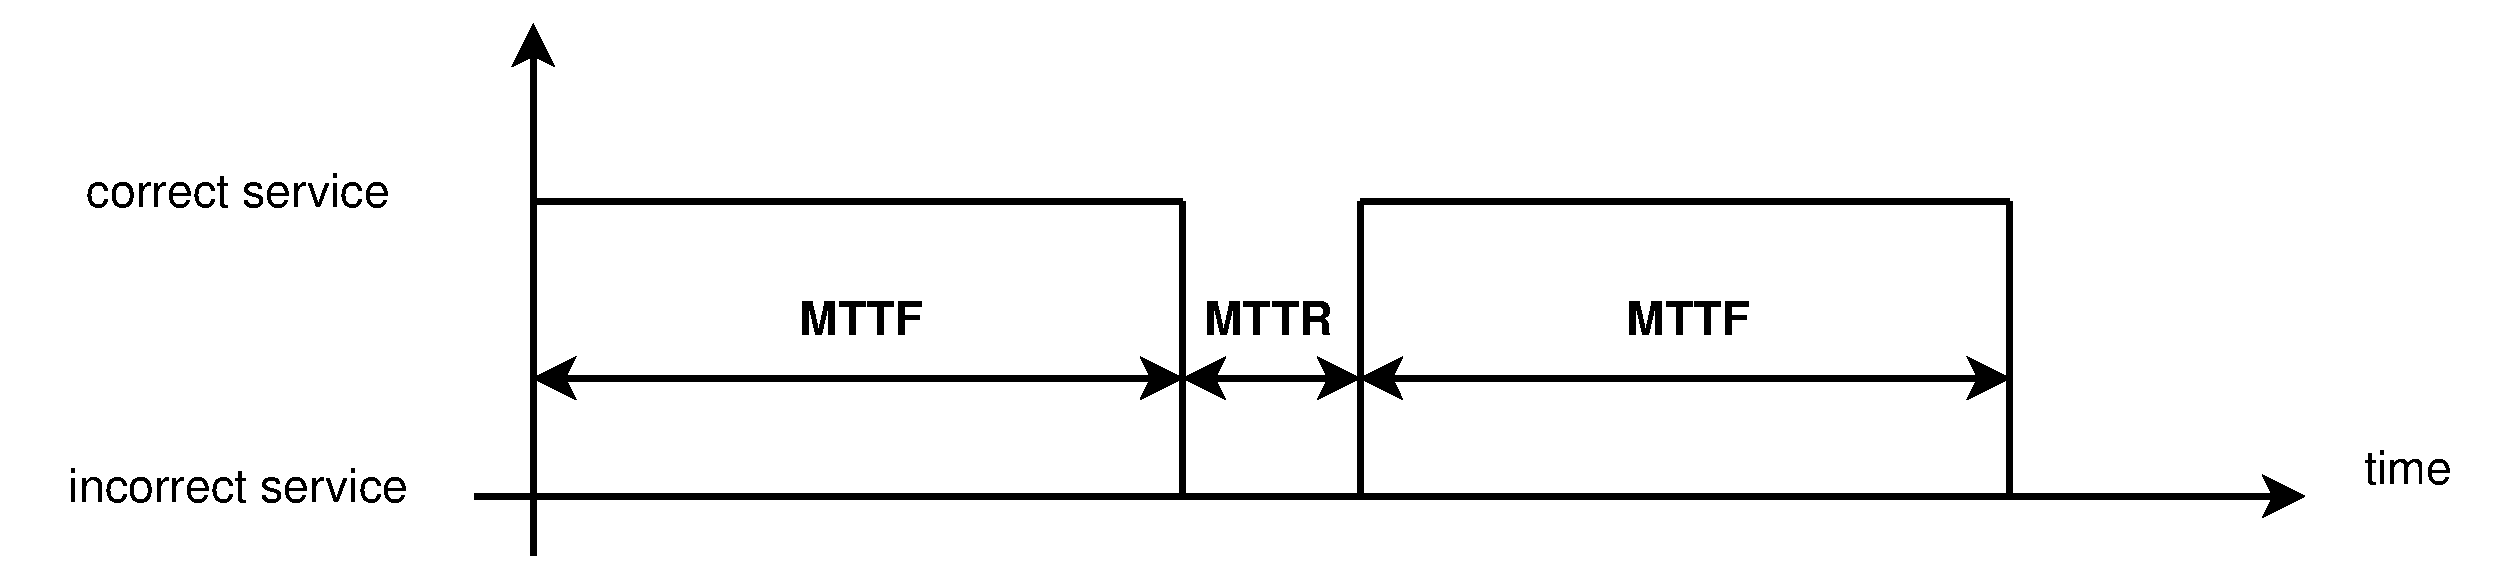
\includegraphics[width=1\textwidth]{figures/availability.eps}
    \caption{Relationship between MTTF and MTTR}
    \label{fig:relmttfmttr}
\end{figure}
%\begin{center}

\begin{table}
\centering
\begin{tabular}{ c | c c  }
  x & $P_{availability}$ & failure duration per year \\ \hline
  1 & 90,0000    & ~ 36 days \\
  2 & 99,0000    & ~ 3,5 days  \\
  3 & 99,9000    & ~ 9 hours \\
  4 & 99,9900    & ~ 1 hour \\
  5 & 99,9990    & ~ 5 minutes \\
  6 & 99,9999    & ~ 31 seconds \\ 
\end{tabular}
\caption{Availability in x-9 notation}
\label{table:x-9}
\end{table}
%\end{center}
For a system with 6-9 availability, this would mean that the system provider assures that the system will be unavailable not more than about 31 seconds over a
whole year.
\\
\\
Availability is important simply because unavailable systems cause costs. Because of the relation of availability to reliability and the maintainability
of the system, as shown in Equation \ref{EQUavailability} and Figure \ref{fig:relmttfmttr}, two options to improve availability exist: either increasing
the \gls{mttf} (i.e. increasing reliability) or decreasing \gls{mttr}.
%An informal definition of a dependable system is a system which delivers a service that can be justifiable trusted. More formally,
%dependability consists of the following attributes:
%\textit{Availability}, which means that the system is ready for correct service, \textit{reliability}, the continuity of correct service,
%\textit{safety}, i.e. the avoidance of catastrophic consequences \textit{integrity}, s.t. the system cannot be modified in an unwanted manner
%and \textit{maintainability}, so that the system can be repaired in the case of a failure.
%In case of a secure system, another important property is \textit{confidentiality}, which means that no information is disclosed to unauthorized 
%entities.
\begin{align}\label{EQUavailability}
 P_{Availability} = \frac{t_{correct\ service}}{t_{total}} =  \frac{{\gls{mttf}}}{\gls{mttf}+\gls{mttr}}
\end{align}
Reliability measures the probability that the service will work as expected until time $t$:
\begin{align}\label{expFailLaw}
 R(t) = e^{-\lambda(t-t_0)}
\end{align}
Equation \ref{expFailLaw} is known as the \textit{exponential failure law}, $\lambda$ denotes the failures per hour, its inverse $\frac{1}{\lambda}$ is
called \gls{mttf}. Reliability can also be expressed in terms of \textit{un}reliability, denoted $Q(t)$:
\begin{align}
 Q(t) = 1 - R(t)
\end{align}
Maintainability measures the time that is needed to repair a system, with $\mu$ denoting the repair rate and $\frac{1}{\mu}$ called \gls{mttr}.
\\
\\
Every system will most likely consist of different and distinct components, each with its own reliability and failure rates. The final system
will possess an overall reliability, determining its availability. To model the resulting system, the components will be put together in a mixture of
serial and parallel systems.
\begin{figure}
    \centering
    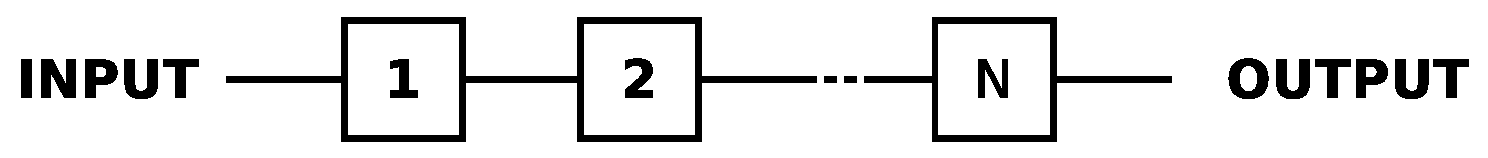
\includegraphics[width=0.8\textwidth]{figures/seriesSystem.eps}
    \caption{Model of a series system}
    \label{fig:serSys}
\end{figure}
For example, if all $i$ components, ranging from $1$ to $N$, are necessary to work correctly for the overall system to deliver correct service, this can be modeled as
a series system, see Figure \ref{fig:serSys}. This does not mean that the components are necessarily connected in a serial way, it just stresses that failure
of one single components breaks the whole system. System's reliability then equals the product of all component's reliabilities:
\begin{align}
R_{system}(t) = \prod_{i=1}^{N} R_{i}(t) 
\end{align}
In contrast, a system containing redundant components, failure of one such component must not produce an outage of the overall system. This can be modeled as
a parallel system (as shown in Figure \ref{fig:parallelSys}). Here, the overall reliability can be calculated as given in Equation \ref{parallelSysEqu}.
\begin{figure}
    \centering
    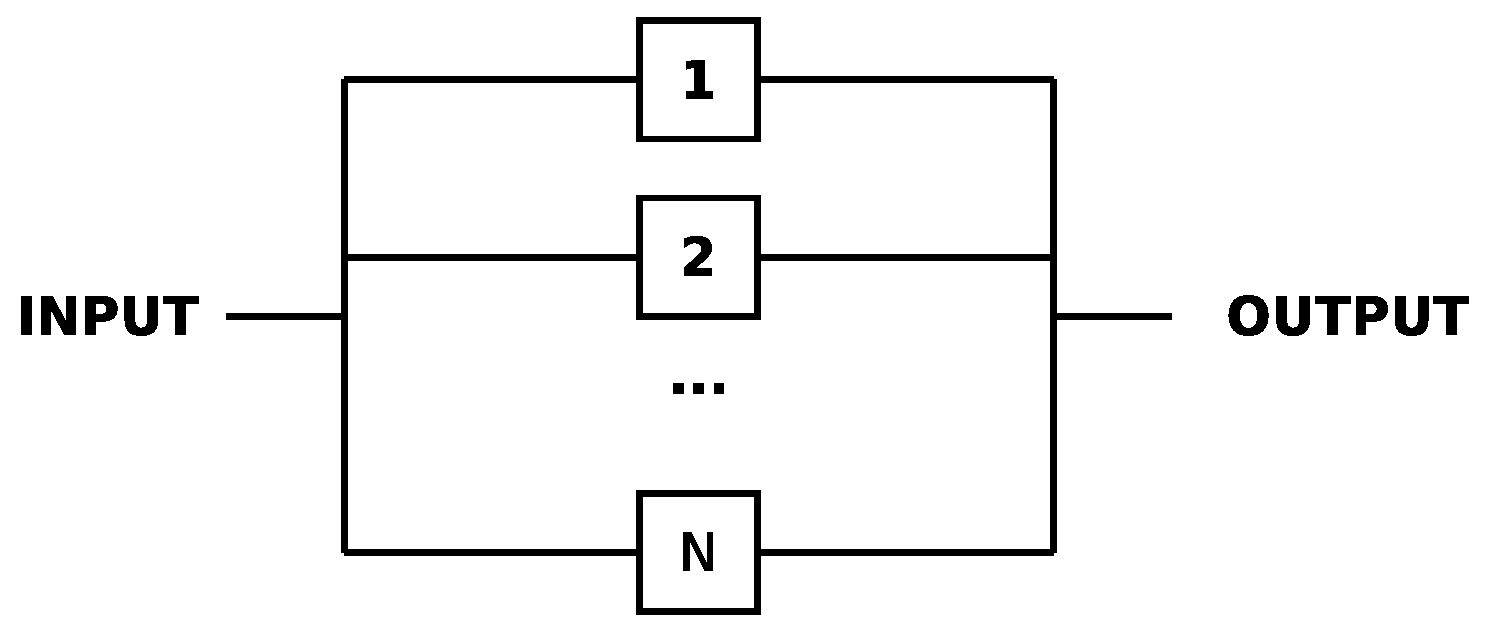
\includegraphics[width=0.8\textwidth]{figures/parallelSys.eps}
    \caption{Model of a parallel system}
    \label{fig:parallelSys}
\end{figure}

\begin{align}\label{parallelSysEqu}
 R(t)_{system} = 1 - \prod_{i=1}^{N} 1- R_{i}(t) = 1 - \prod_{i=1}^{N} Q_{i}(t)
\end{align}
Mixed systems, containing paralell and series system, can be calculated by iteratively condensing serial- or parallel subsystems into single components,
as shown in Figure \ref{fig:mixedSys}.
\begin{figure}
    \centering
    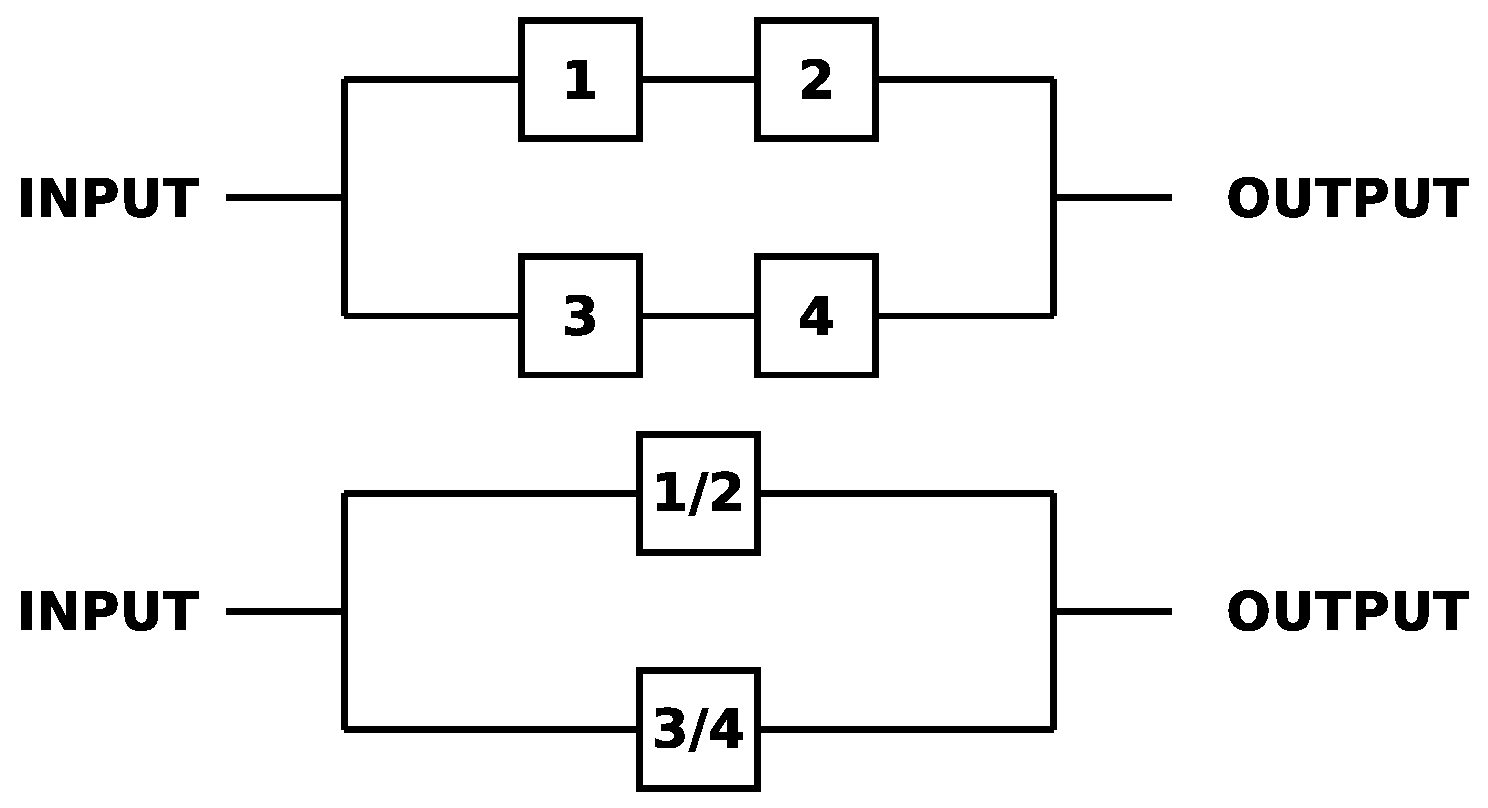
\includegraphics[width=0.8\textwidth]{figures/mixedSys.eps}
    \caption{Condensing a mixed system}
    \label{fig:mixedSys}
\end{figure}
\\
\\
\gls{ha} characterizes a system that is designed in a way to avoid outages, or in case of a failure that can be repaired in shortest possible time. 
The level of the needed availability depends on the environment of the system and must be weighted against the additional costs, introduced by improving availability.
Therefore, no hard definition for \gls{ha} can be given - it is a design goal and depends on the context. Availability requirements will most certainly be higher
for systems in safety-critical requirements. A safety-critical system must not fail, otherwise endangering human lives or 
causing substantial economic loss or environmental damage \cite{1007998}.
On the other side, systems that will produce only minor costs when not operating correctly
will probably have to meet less stringent availability levels.
\\
For example, our society heavily depends on electric power supply, an outage
is nearly unacceptable. On the other side, it is impossible to guarantee 100\% availability, so if a power outage occurs, the system must be fixed as soon as
possible to restore correct service, otherwise risking human lives. On the contrary, a booking system will obviously result in financial losses for the company 
if not working, but no more serious consequences are to be assumed.
\\
\\
This work's focus lies on security-critical systems, increasing availability of KNX networks, but restricting its
deployment to environments without safety-critical needs. Thus, safety criticality is neglected here because of its most stringent demands, as needed in
avionics or weapons systems.
The difference between safety-critical and security-critical systems can be given as follows \cite{5784222}: safety means that software must not be harm the 
world (i.e. containment), while security means that the world must not harm software (i.e. protection).

\section{Failure Avoidance}

Different strategies exist to handle faults, thus trying to avoid that a fault propagates through the system and finally leads to a system failure.
These strategies are introduced in the next section.

\subsection{Fault Removal}
Fault removal tries to identify faults by testing the system before its deployment. 
\\
Therefore, the system is exposed to test cases, which ideally would cover all possible internal states. Whenever a failure occurs, the erroneous state is identified, the
underlying fault is removed and a new testing cycle begins.
\\
A problem about this approach is the huge test space that for even simple systems would be required to iterate through. Therefore, the method suffers from the very
fundamental dilemma that testing never can proof that a system is fault free.
\subsection{Fault Avoidance}
Fault avoidance aims at producing a system which is fault-free
per design and is applied at the design stage of the system. Despite the methods for achieving fault avoidance can be applied in the domain of sofware and hardware,
they can not guard against transient hardware faults occurring after the system is deployed.
\\
Fault avoidance is based on two distinct processing steps: validation and verification. Validation is used to show that the specification, which is
the basis of system implementation, matches the real world within reasonable borders. This is necessary because every human built system uses an abstraction
of the real world, thus simplifying the model.
\\
In contrast, verification assures that the system indeed matches the specification. In other words, validation tries to answer if the correct system was built,
while verification is concerned about to build the system correctly.
\\
\\
Formal methods can be be utilized for verification if the system model is available in a formal language. The formal properties of the specification can then be 
checked automatically against a finite-state model of the system, a method called \textit{model checking}.
\\
While automatic validation can proof that the resulting system is correct in regard to the specification, a big problem here is to obtain the formal properties
out of an informal specification.
\\
\\
\\
Obviously, both fault removal as well as fault avoidance cannot handle deliberately introduced faults, caused by an active adversary.
Additionally, they cannot deal with hardware errors -  therefore it is argued that fault tolerance is the only practical way to guarantee availability
in a hostile environment (i.e. an environment where active attackers are assumed to exist and therefore \gls{dos} attacks cannot be ruled out), as well as to
protect against random hardware errors.
\\
Consequently, the proposed solution will be based on fault tolerance to achieve \gls{ha}, which will be examined more detailed.
 
\subsection{Fault tolerance}
Fault tolerance tries to ensure correct service despite the occurrence of faults and is achieved through error detection and subsequent system recovery.
To enable error detection, redundancy is added to a system and thereby the 
system's complexity is increased. This can be achieved both in the domain of hardware and software. 
\\
The basis of the design of fault tolerant systems is the definition of a \textit{fault hypothesis}, stating which faults must be tolerable by the system, thus
dividing the fault state into normal faults and rare faults (i.e. faults not covered by the fault hypothesis). Normal faults can be corrected by the fault-tolerance
mechanism. 

\subsubsection{Fail-silent fault tolerance}
Fault tolerance can be achieved based on \textit{fail-silent} components. A fail-silent component
either works correctly, i.e. outputs correct values, or does not output any values at all \cite{544479}. By duplicating such a module and comparing the
outputs, fault tolerance can be achieved by cutting off the faulty module from the system.
\\
This method is used for example for \gls{raid} based date storage \footnote{although the logic distributing
the data chunks to different devices can be built in hardware or in software, i.e. the operating system, \gls{raid} always relies on redundant disks}.
For \gls{raid} level 1, all data to be stored is duplicated to two independent disks. In case a hardware failure of one drive is detected, the data can be accessed
from the second drive. This method does obviously not work if both drives seem operable, but one drive outputs bogus data, i.e. it is not acting fail-silent.
To handle this situation, higher redundancy levels are needed, as implemented for example in \gls{tmr}. 

\subsubsection{\gls{tmr}}
A \gls{tmr} system, see Figure \ref{fig:tmr}, is composed out of 3 modules or \textit{black boxes}, all performing the same task,	
and one \textit{majoriy organ} $V$, as proposed by Von Neumann \cite{vN56}. The latter element
is also called \textit{voter} because out of its 3 inputs, it chooses the 'correct' output based on majority voting. As long as at least 2 black boxes do not
fail, the system can provide correct service. If it is assumed that the voting element has perfect reliability = 1 and all black boxes $M$ are independent from
each other and have reliability $R_M$, the overall, time-invariant system's reliability is given in Equation \ref{tmrEq} \cite{Lyons:1962:UTR:1661979.1661984} and plotted in Figure \ref{fig:tmrGrp}
\begin{align}\label{tmrEq}
 R_{system} = {R_M}^3 + 3{R_M}^2(1-R_M) = 3{R_M}^2 - 2{R_M}^3
\end{align}
\begin{figure}
    \centering
    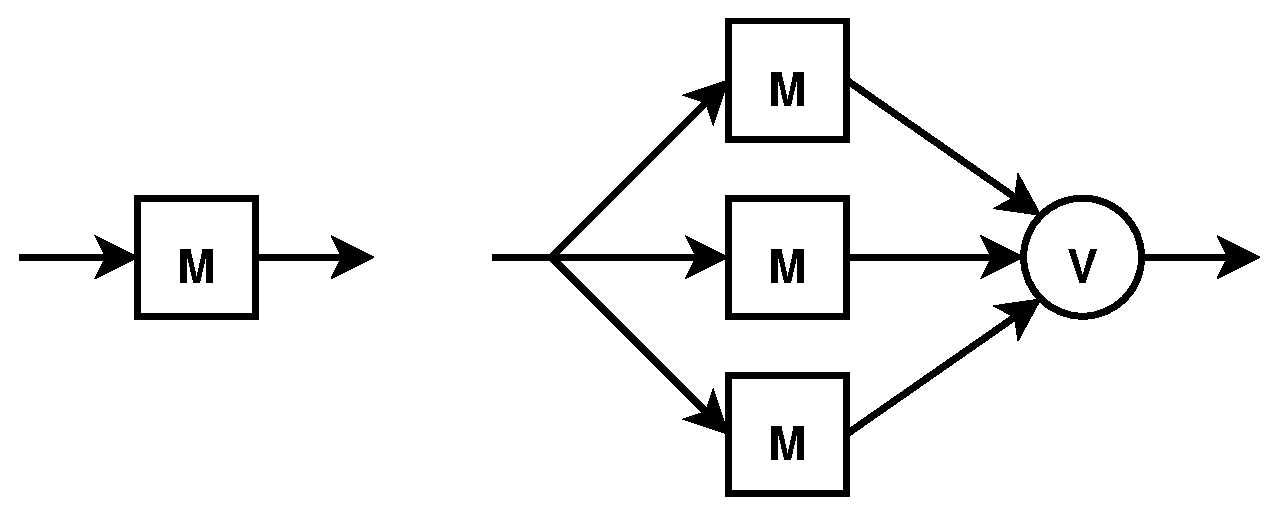
\includegraphics[width=0.8\textwidth]{figures/tmr.eps}
    \caption{Non-redundant operation vs. \gls{tmr}}
    \label{fig:tmr}
\end{figure}
\begin{figure}
    \centering
    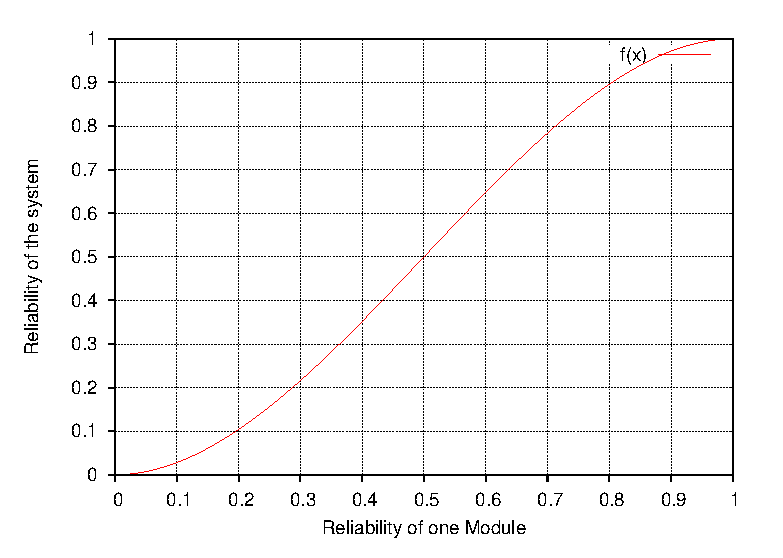
\includegraphics[width=0.8\textwidth]{figures/tmrGraph.eps}
    \caption{Reliability of resulting system}
    \label{fig:tmrGrp}
\end{figure}
It can be seen that if $R_M \leq 0.5$, overall reliability even gets worse, while for components reliabilities nearly being unit, very high system reliability can
be achieved.
\\
\\
The concept of \gls{tmr} can be generalized to $n$ devices performing
the same operation. In most cases $n$ will be odd, so failure of up to $\frac{n-1}{2}$ modules can be tolerated.

\section{Fault Tolerant Technologies}
In the next sections, communication protocols based on ethernet, satisfying the needs of industrial communication networks, are examined. Beside the need for high availability,
industrial production lines
are sensitive against network disruptions. While, depending on the application domain short interruptions in the range of milliseconds to seconds may be
tolerable, longer outages will force emergency stops or even cause damage.

\subsection{Network redundancy}

Communication networks can be modeled as graphs. A graph, as shown in Figure \ref{fig:graph}, is an ordered pair $G=(V,E)$, with $V$ being the set of vertices and $E$
the set of edges, connecting the vertices. For a weighted graph, every edge is associated to a \textit{cost}. 
\\
A \textit{closed walk} or \textit{cycle} exists if a path from one vertex to itself exists, resulting in multiple paths from one node to others.
Such a network posses intrinsic redundancy, a fact that can be exploited to gain fault tolerant systems.
\\
If the graph is undirected, every line determines a bidirectional communication link. 
\\
A spanning tree of graph $G$ is a subgraph $T$, possessing all vertices $V$ but only a subset of the edges $E' \subseteq E$ s.t. all vertices are reachable,
but no loops exists. In the case of a weighted graph, the weight of the spanning tree is the sum of all existing edges.
\begin{figure}[H]
\centering
 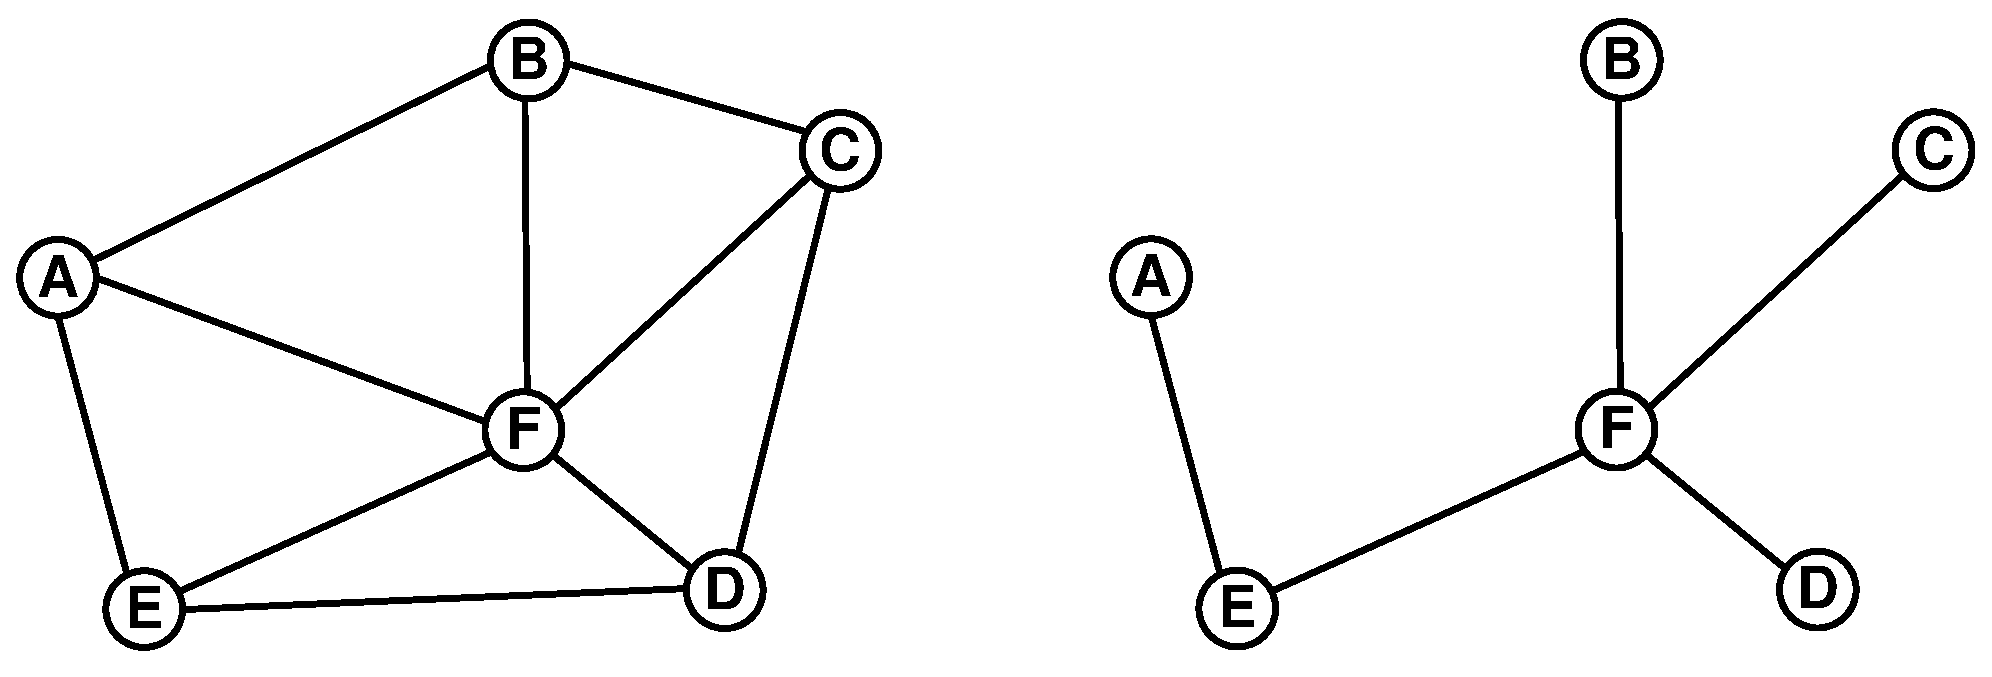
\includegraphics[width=0.8\linewidth]{figures/graph.eps}
 \caption{Undirected graph, spanning tree of the graph}
\label{fig:graph}
\end{figure}

\subsubsection{\gls{stp}}
The widely used \gls{ieee} 802.3 ethernet standard was not designed with high availability in mind.
Nevertheless, it already provided basic fault tolerance mechanisms based on the \gls{ieee} 802.1D \gls{stp}. 
\\
\\
In typical ethernet installations, depending on the network topology different
nodes may be reachable through different paths, i.e. physical loops may exist.
Switches, operating at \gls{osi} layer 2, are responsible for loop detection and
loop prevention. They must logically disconnect such loops by blocking the corresponding ports to protect the network,
as required by the ethernet specification, because multicast or broadcast traffic, generated by one of the connected
devices, will be forwarded by all switches on all ports (except the incoming ports). This would flood the network until no regular communication will be possible any
more.
\\
\begin{figure}[H]
 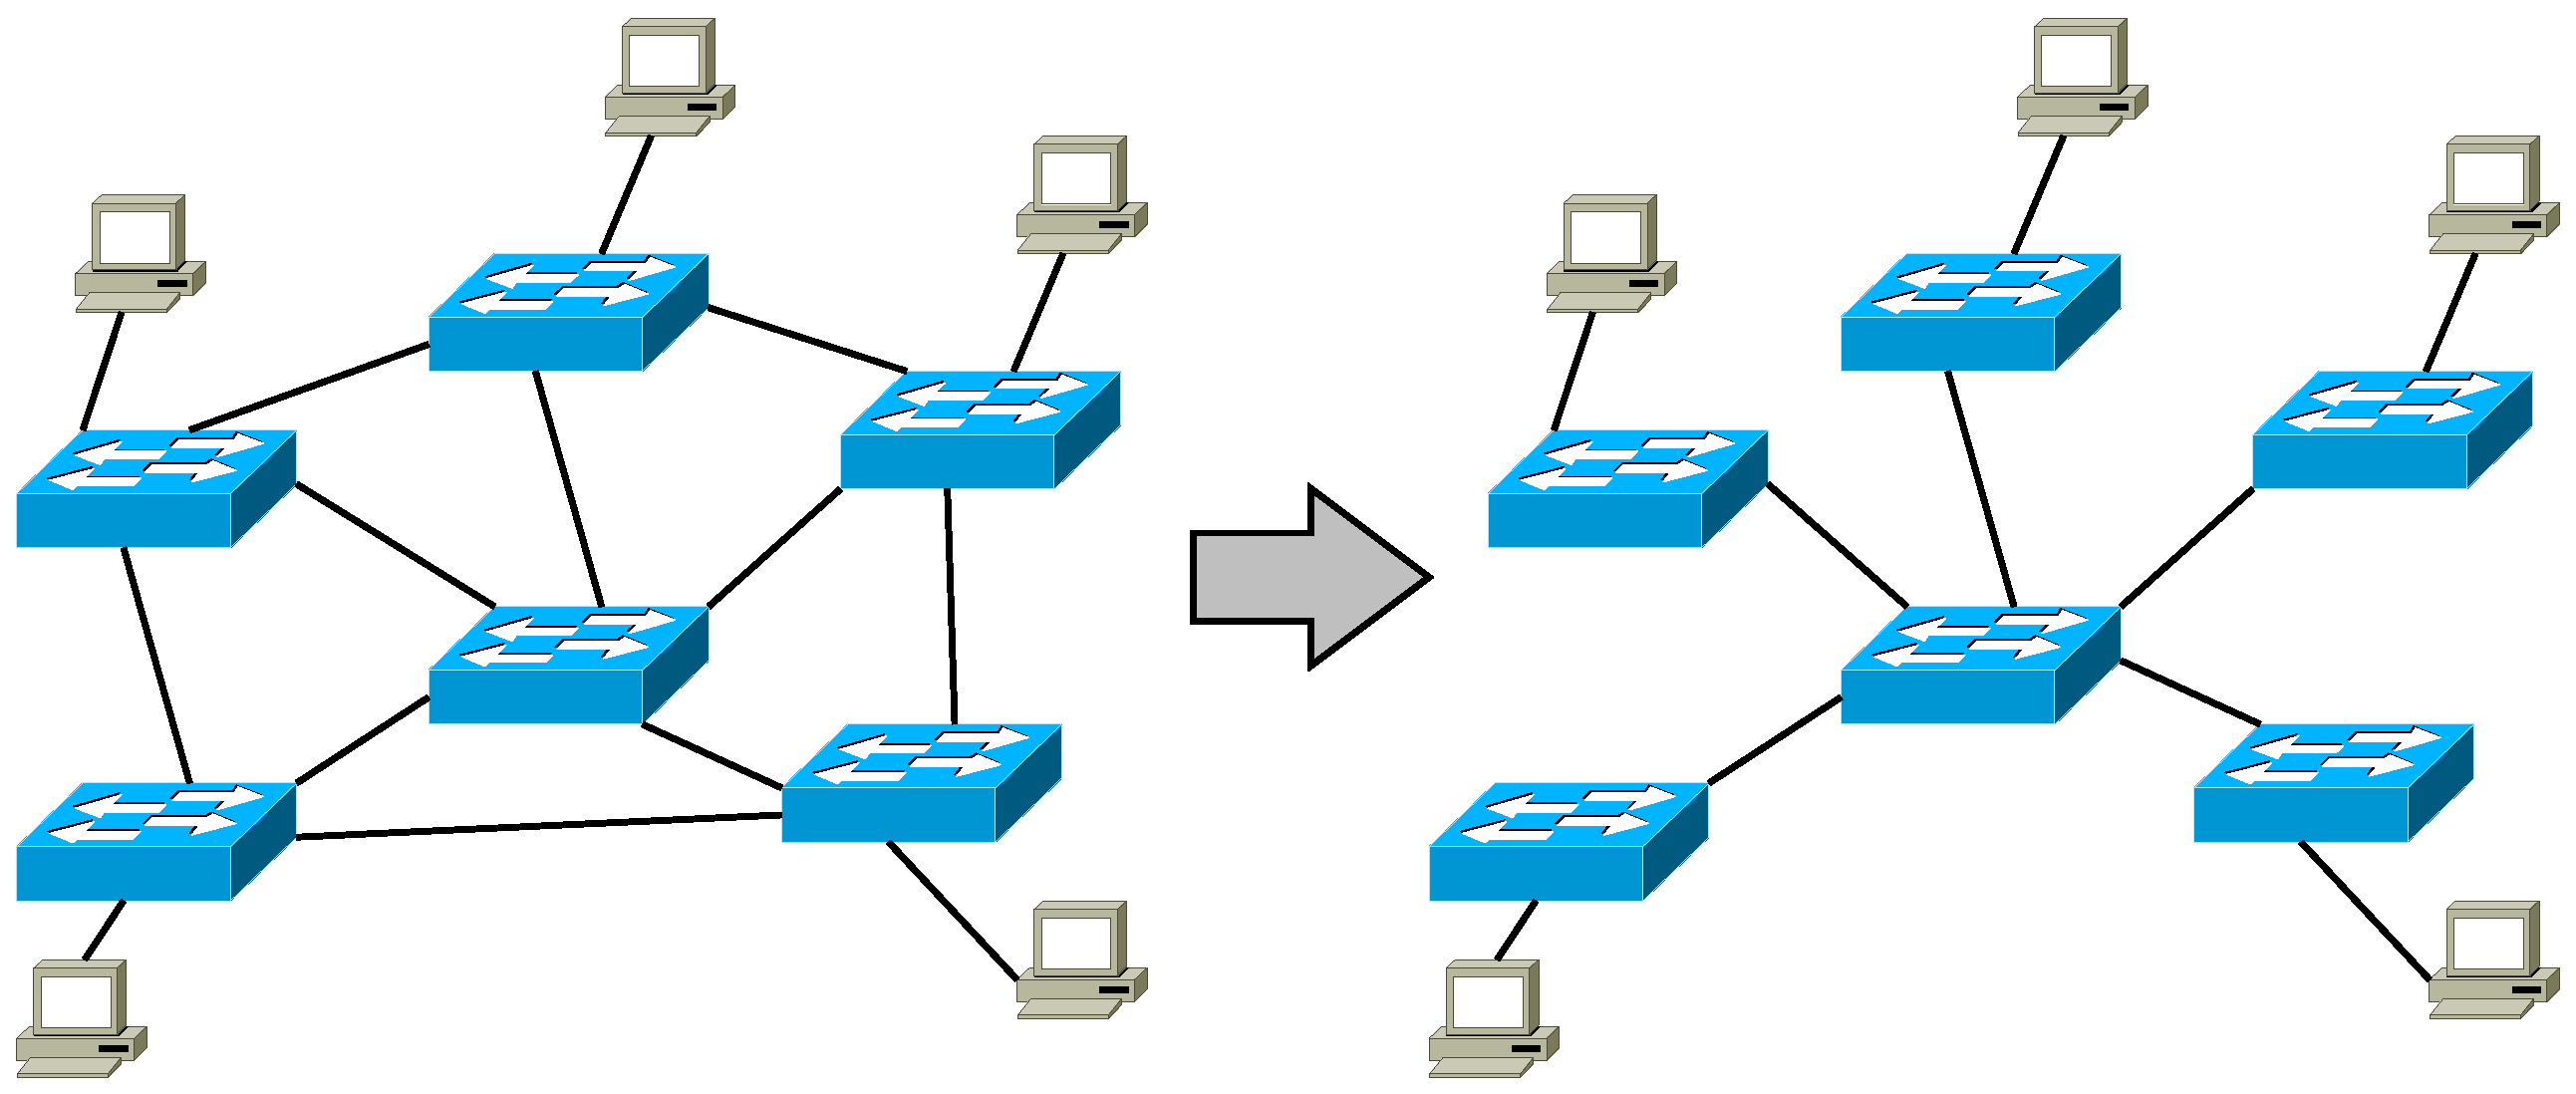
\includegraphics[width=\linewidth]{figures/stp.eps}
 \caption{Protecting ethernet segments from loops with \gls{stp}}
\label{fig:stp1}
\end{figure}
This situation is shown in Figure \ref{fig:stp1}: on the left side, the physical connections are shown, containing loops. 
\gls{stp} removes
the loops by setting certain interfaces to blocking mode, connected by dotted lines, as shown on the right side of Figure \ref{fig:stp1}.
\\
The algorithm works as follows:

\begin{itemize}
 \item The first step of the \gls{stp} algorithm is to nominate one device as root bridge\footnote{the terms \textit{switch} and \textit{bridge} are used synonymously,
with the major difference that switches can break network segments into multiple subsegments through \glspl{vlan}}. This can be done manually by the network administrator,
or dynamically through the exchange of packages containing a priority. All switches will agree on lowest priority device as root bridge, additionally using the unique
hardware \gls{mac} address if collisions occur. The root bridge sets all interfaces to forwarding mode. 
 \item Afterwards, every switch determines the path with minimal costs for reaching the root bridge. The cost of every connection can be determined by the link
 speed or configured by the network administrator manually.
 \item Finally, all devices except the root bridge set the ports belonging to the minimal-cost path to forward mode. All other ports are set to blocking mode, thus removing
 any loops.
\end{itemize}
If a connection is lost and an ethernet segment is not 
reachable any more, the \gls{stp}, although not primarily designed for that tasks, can be used to handle that fault. Nodes affected by the link-change report
that event to the root bridge, so that the network can be re-configured and a different path can be established, thus re-connecting the unreachable segment
and providing fault tolerance. 
\\
\\
A big drawback of this mechanism is the topology-dependent
time needed for network re-organization. While in simulations delays of millisecond magnitude can be achieved \cite{4447112}, in practice link recovery
can take up to one minute which is not acceptable for many industrial environments. An improvement was achieved with \gls{ieee} 802.1w \gls{rstp} and
a variety of different proprietary protocols, not compatible to each other, but still no sufficient recovery times were achieved \cite{1704183}.

\subsubsection{IEC 62439}

As it turned out that the mechanisms based on \gls{stp} and its variations were not 
sufficient for many applications, the family of IEC 62439 standards was defined. IEC 62439 introduces a set of ethernet extensions, assuring high availability
and enabling its deployment in industrial applications. Three extensions are introduced below.

\subsubsection{\gls{mrp}}
After IEC 62439-1 specifying basic definitions, the second draft introduced \gls{mrp} which confines network outages to less than 500ms \cite{6145654}.
This is achieved by restricting the valid topologies to ring-only, so all switches are connected to the network by 2 interfaces. All switches, beside the ring manager,
forward all traffic received, while the ring manager opens the loop logically by setting one of its interfaces to blocking mode.
In this mode, all packages except management messages are discarded. The ring manager detects a failure by periodically sending test management messages in both
directions. Additionally every node is able to detect a link failure on its local ports. It then sets the port to blocking and signals this link failure to the
ring manager which opens his second port by setting it to forward mode and therefore reconnects the unreachable segment.
\\
\gls{mrp} does not rule out package loss in case of a failure, therefore it can be seen as improved \gls{rstp} for ring topologies. 

\begin{figure}[H]
 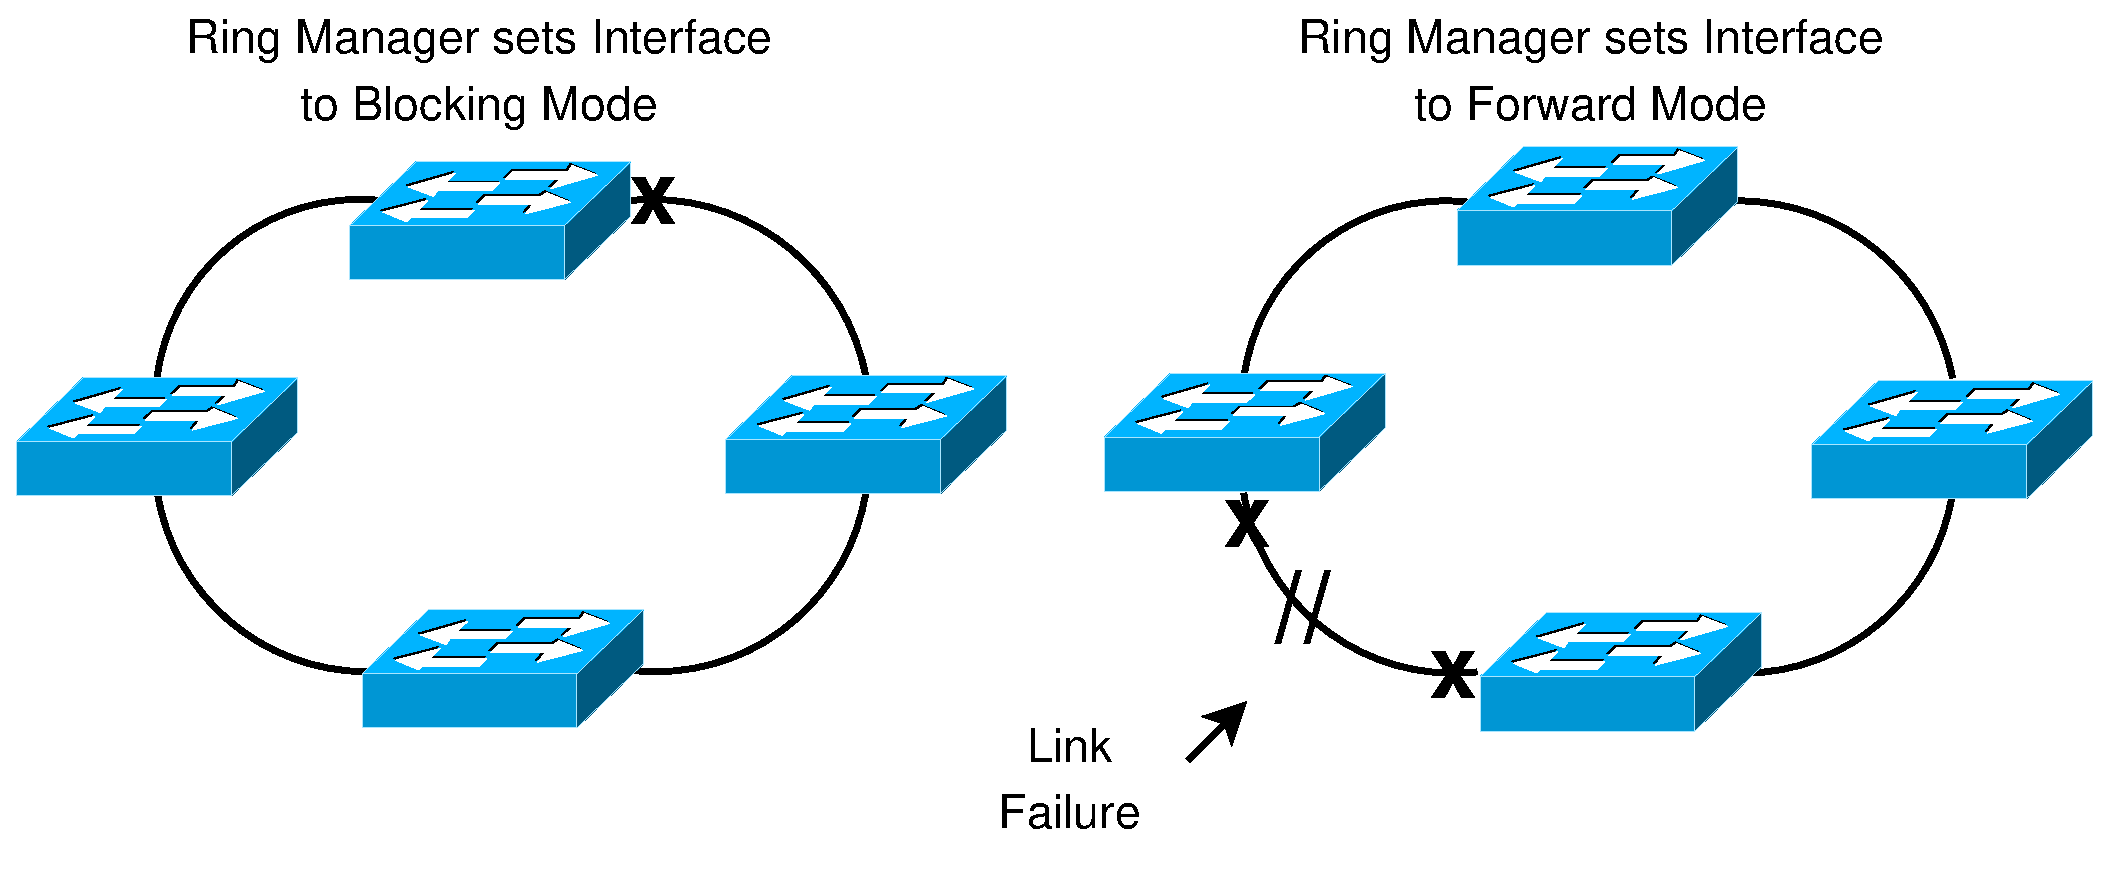
\includegraphics[width=\linewidth]{figures/MRP2.eps}
 \caption{MRP fault tolerance}
\label{fig:mrp1}
\end{figure}


\subsubsection{\gls{prp}}
In 2010, IEC 62439-3 defined a first version of {\gls{prp}} and \gls{hsr}, both suitable for hard real-time
systems \footnote{hard real-time characterizes a system where missing of a dead line may result in a catastrophic event} \cite{4416946}.
\\
In 2012, IEC 62439-3 was revised, defining new versions of \gls{prp} and \gls{hsr}. The basic ideas behind both protocols remained
unchanged, so the latest versions are described below.
\\
\\
\gls{prp} can tolerate a link fault without package loss by utilizing two redundant and independent \glspl{lan}.
Nodes needing high availability, called \gls{danp}, are connected to both networks by two interfaces, sharing the same \gls{mac} and \gls{ip} addresses.
Additionally, standard ethernet devices called \gls{san} can be connected to only one network, enabling communication with devices on the same \gls{lan} only.
An example of such a network is shown in Figure \ref{fig:prp}.
\\
To support redundant connections for \glspl{danp}, a sub-layer on \gls{osi}-layer 2 (i.e. the link layer), called \gls{lre} is defined. 
Upper level data arriving at the \gls{lre} of a \gls{danp} is duplicated and equipped with 6 bytes of control information, containing a 2 byte sequence number,
\gls{lan} number, length information and a static suffix identifying the \gls{lsdu} as \gls{prp} traffic. The sequence number is used for duplicate detection: 
every node uses one global counter $Ctr_{global}$ for outgoing messages, not discriminating the receiver. For every package sent, the sequence number is incremented.
Additionally, every node maintains distinct counter values $Ctr_{source}$ for every unicast source-address it receives messages from, as well as for multicast
and broadcast messages.
\\
On the receiving side the \gls{prp} traffic is detected because of the suffix, duplicates can be discarded by utilizing the sequence number \cite{6699852}.
The standard does not dictate how this must be achieved, it only demands that legitimate packages must not be discarded. Because of the short global outgoing 
sequence number, duplicates may not be detected as such - responsibility for final detection is delegated to upper layers.
%If the received number is higher than the saved one $C_{source}$, the package is forwarded to the upper layer and the received sequence number is saved as $C_{source}$.
%Therefor, the package transmitted over the alternate line (i.e. the delayed package) will contain a sequence number smaller than the number saved for the 
%corresponding source address and can safely be discarded, thus preventing the processing of duplicate frames by the upper level.  
\begin{figure}
    \centering
    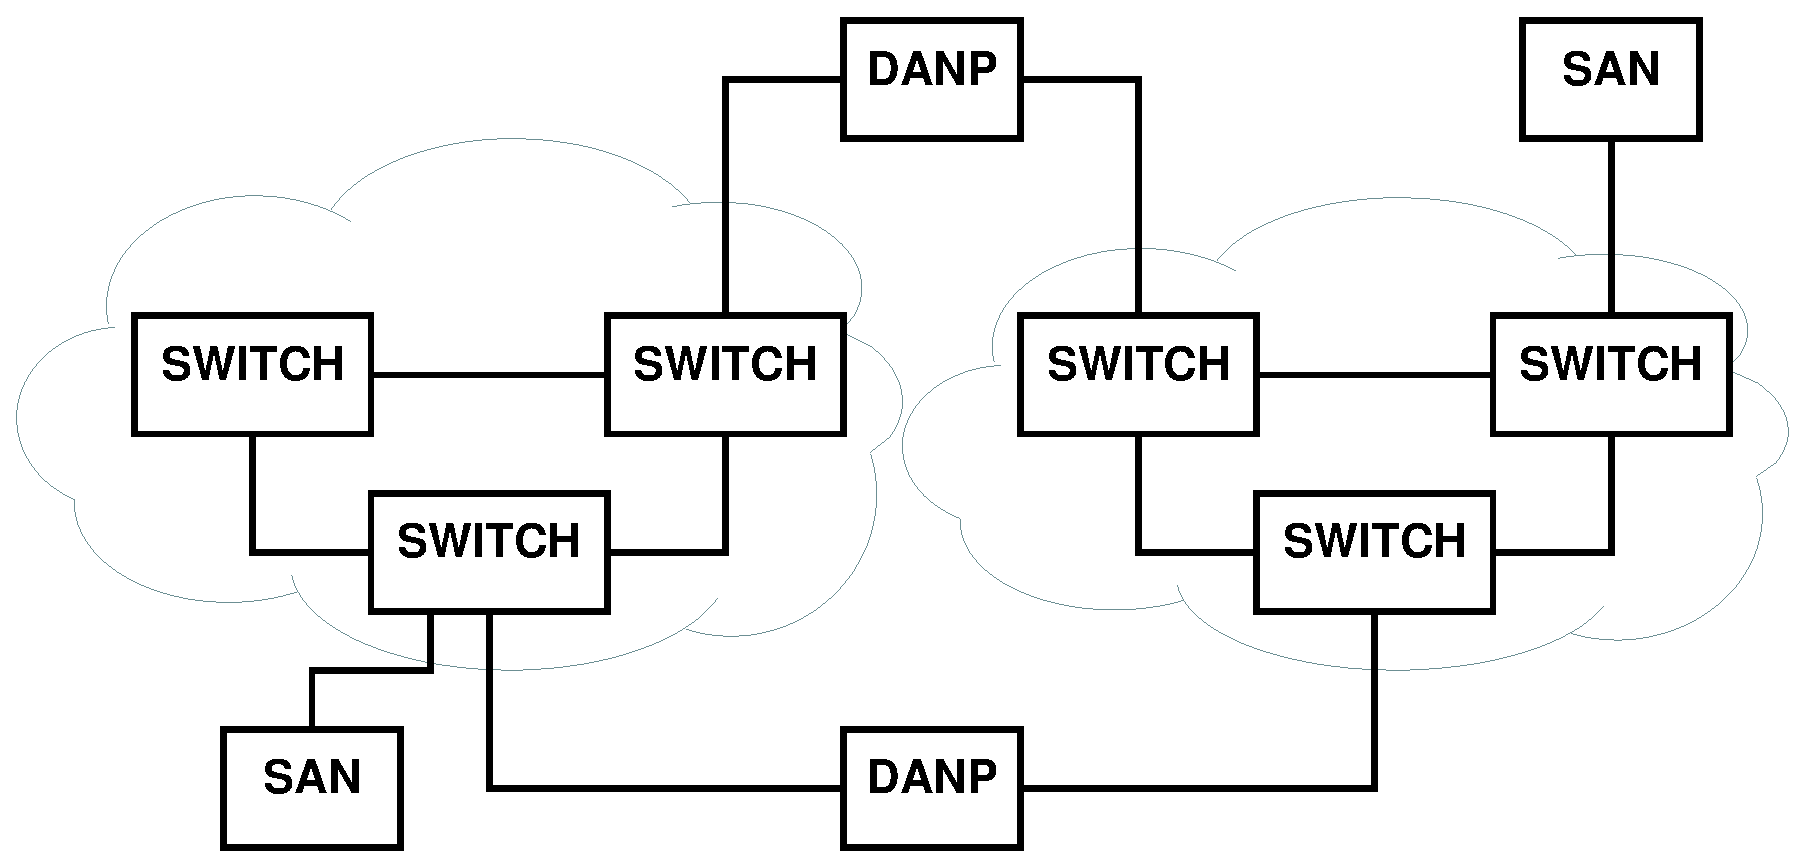
\includegraphics[width=1\textwidth]{figures/prp.eps}
    \caption{\gls{prp} network}
    \label{fig:prp}
\end{figure}

\subsubsection{\gls{hsr}}
\gls{hsr} is based on ring-topology, but it also allows to connect \gls{hsr} and \gls{prp} networks, different \gls{hsr} rings or even to build a ring of rings. 
Every node is connected to the network by two interfaces, duplicating data from upper layers and sending one copy in clockwise, the other copy in counter-clockwise direction,
thus eliminating the need for duplicated networks but wasting about half of the available bandwidth \cite{6174793}. 
\\



%%%%%%%%%%%%%%%%%%%%%%%%%%%%%%%%%%%%%%%%%

%%%%%%%%%%%%%%%%%%%%%%%%%%%%%%%%%%%%%%%%%
\chapter{KNX}
\label{ch:knx}
\label{chap3}
\section{Introduction}

\gls{knx} \footnote{connexio, latin for connetion} implements a specialized form of automated process control, dedicated to the needs of \gls{hbas}. \gls{knx}
emerged from 3 leading standards namely the \gls{eib}, the \gls{ehs} and BatiBUS. It is an open, platform independent standard,
developed by the KNX association implementing the EN50090 standard for home and building electronic systems.
\\
To provide platform independence, the standard uses a layered structure, based on the \gls{iso} / \gls{osi}. Different kinds of physical backends are supported,
allowing its use in different environments.
\\
\gls{eib} already supported interoperability between products from different manufacturers. This was achieved by
the definition of the \gls{eis}, which standardizes
the data transported inside the datragrams. \gls{knx} continued this efforts with the introduction of common \gls{dt}, distinguishable through unique ids, thus
standardizing their encoding, format, range and unit.
Every \gls{dt} groups related \glspl{dpt}, the actual control variables of the network, together, allowing 
\\
For example, every \gls{knx} 
certified manufacturer producing a switching actuator must use the defined dataformat - an end-user can therefore exchange such an actuator without caring
about compatibility issues. For configuration and parametrization of the devices, a Windows based software suite called \gls{ets} is used, which also offers
a bus monitor for debugging.

\section{KNX layers}\label{sec:knxLayers}

The \gls{osi} standardizes the communication between different, independent systems
by grouping the needed functions into 7 sublayers to provide interchangeability and abstraction. Every layer provides services to its next-higher layer, and
uses the services provided by its next-lower layer. Every service is defined by standardized interfaces - that way any layer can be modified internally without
compromising the function of the system, as long as the defined interfaces are implemented. This fragmentation of one service follows the paradigm of 
\textit{impera et divide} \footnote{latin for: divide and rule} and facilitates the building of complex systems by dividing one complex problem into subsequent,
less-complex problems.
\\
\gls{knx} implements this model, omitting 
layers 5 and 6, as shown in Figure \ref{fig:knxlayers}. Data from applications are directly passed to the transport layer in a transparent way, and vice versa.
\begin{figure}
    \centering
   % 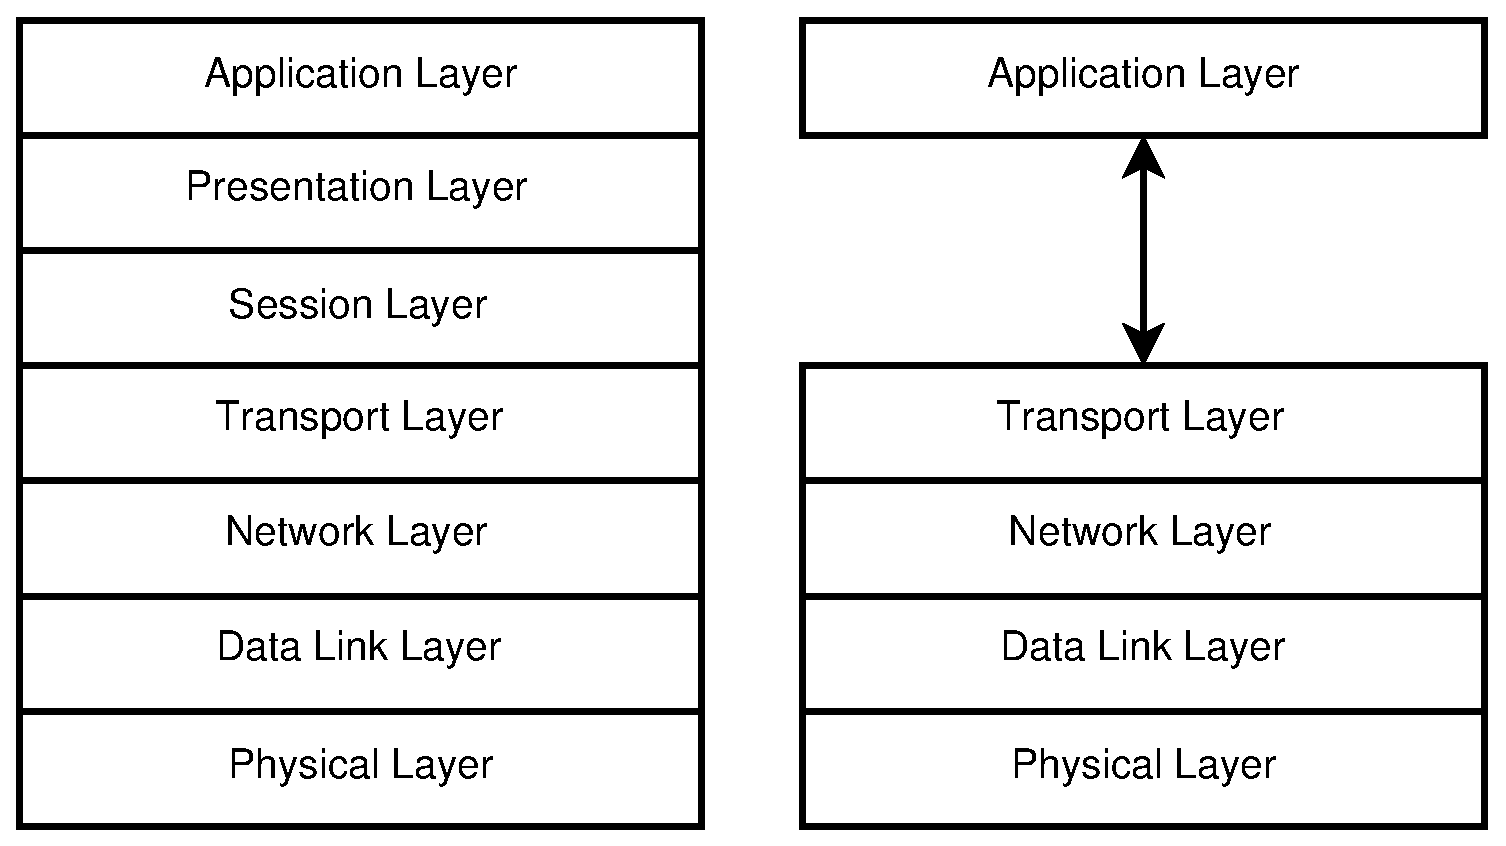
\includegraphics[width=0.7\textwidth]{figures/KNXvsISO.eps}
     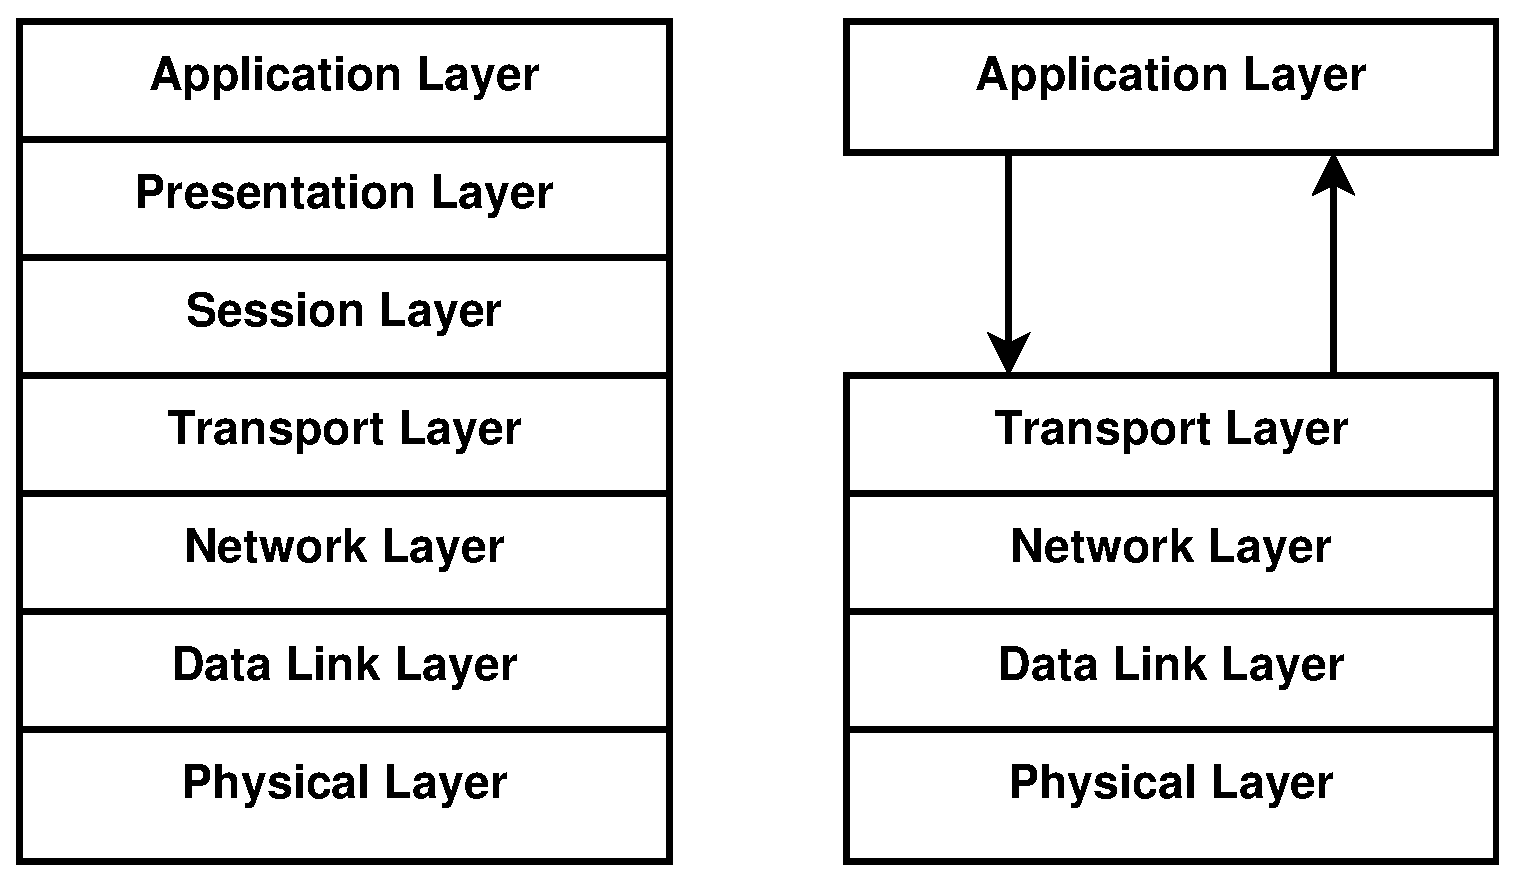
\includegraphics[width=0.7\textwidth]{figures/isoOSI.eps}

    \caption{OSI Layer Model, compared to the \gls{knx} Model}
    \label{fig:knxlayers}
\end{figure}

\subsection{Physical layer}
This is the lowest layer as defined by \gls{osi} and determines the basic transmission parameters like symbol rate, signal form but also mechanical 
characteristics like which connectors are used.
\\
\\
To provide flexibility in \gls{knx}, four different physical media are defined. \gls{TP}-1 which was inherited from \gls{eib}, and is the successor of \gls{TP}-0,
as defined by BatiBUS, is the basis medium, consisting of a twisted pair cabling. Data and power can be transmitted with one pair, so low-power
devices can be fed over the bus. Data transfer is done asynchronously, with bidirectional, half-duplex
communication and a datarate of 9600 \gls{bps}. \gls{TP}-1 uses collision avoidance, and allows all topologies beside rings. 
\\
Because this work is base on the \gls{TP}1 - part of \gls{knx} only, this medium will be explained in more detail in the next section.
\\
\\
PL110, which was also inherited from \gls{eib}, uses power line installations for communications. The carrier uses spread frequency shift keying, and can be used 
for bidirectional, half duplex  communication with an even lower data rate of 1200 bit/sec. \gls{knx} \gls{rf} is used for short range wireless communication
at 868,3 MHz. \gls{knx}net/\gls{ip} allows the integration of \gls{knx} into networks using \gls{TCP} / \gls{ip} for communication. Here, three different communication
modes are defined: tunneling mode is used for configuration and monitoring a client device by a \gls{knx}net/\gls{ip} server. Routing mode is used
for connecting \gls{knx} lines over \gls{ip}, while \gls{knx} \gls{ip} is used for direct communication between \gls{knx} devices. \cite{KraInnosec2013}

\subsubsection{TP-1}

The accurate name for this medium is 'Physical Layer type Twisted Pair', with variants
PhL \gls{TP}-1-64 and PhL \gls{TP}-1-256, which is backward compatible to the former one. While the first one allows
the connection of up to 64 devices, the latter one allows up to 256 devices connected in a linear, star, tree or
mixed topology as one physical segment, also called a line.
\\
Bridges do not possess their own address and are used for galvanic separation of physical segments and for extension of TP-1-64 segments to allow up to 256 devices.
Therefore, they acknowledge layer 2 frames received on one side and forward them to their second interface. 
\\
Routers have their own address space and only forward packages received on one side if the destination address is located on the other side of the router.
As well as bridges, they can be used for galvanic separation and they acknowledge frames on layer 2.
A \gls{lc} is a router that integrates up to 16 lines into one logical object called area. A \gls{bbc} is a router that connects
up to 16 areas to one network, thus providing the maximum size of a network consisting of 65536 devices:
\begin{itemize}
 \item up to 256 devices per line
 \item up to 16 lines per area = 4096 devices in 16 lines
 \item up to 16 areas for whole network = 65536\footnote{it is to be noted that the actual number of usable devices is smaller because routers have
 their own address} devices in 16 areas
\end{itemize}
Gateways are used to connect \gls{knx} networks to non-\gls{knx} networks.
\\
\\
A logical '1' is regarded as the idle state of the bus, so the transmitter of the \gls{mau} is disabled when sending a '1', i.e., the analog signal on
the bus consists only of the DC part. \gls{TP}-1 uses \gls{csma}/\gls{ca} for bus access, so every device must listen to the bus and is only allowed
to begin sending when the bus is idle. In the case of a simultaneous transmission start, a logical '1' of one
device will eventually be overwritten by a logical '0' of the other device. The overruled
sender will detect this by continuously checking the state of the bus and has to stop 
transmission. This behavior is be used to implement priority control and is exploited by the next layer.

\subsection{Data link layer for TP1}

This layer is responsible for error detection, retransmission of corrupted 
packages, framing of the higher level packages into suitable frames and accessing the bus according to the rules used by the particular bus medium. 
It is often broken into 2 distinct sublayers, namely the \gls{mac} as bus arbiter and the \gls{llc}, providing a reliable point-to-point datagram service.
\begin{figure}
    \centering
    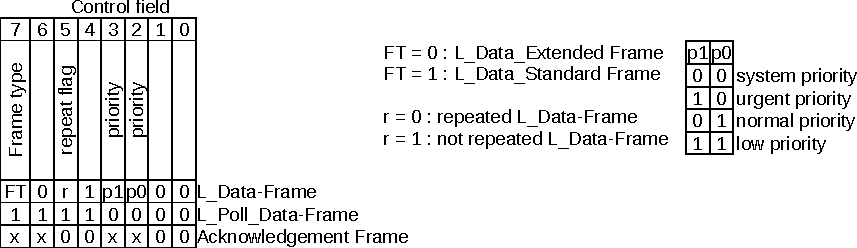
\includegraphics[width=1\textwidth]{figures/ctrl}
%    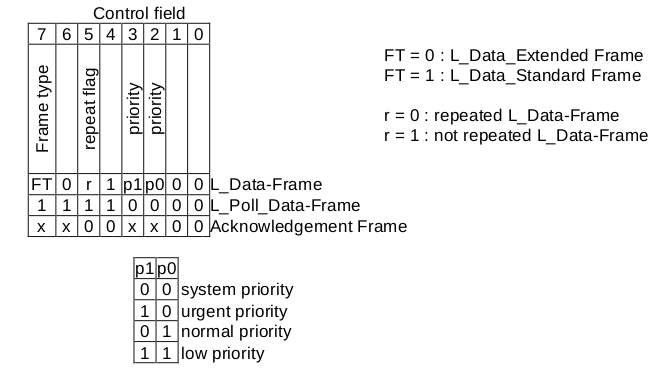
\includegraphics[width=0.5\textwidth]{figures/controlfield.png}
    \caption{Control Field}
    \label{fig:ctrlfield}
\end{figure}
Three frame formats are defined: L\_Data frames are used for sending a data payload to an \gls{ia}, a group address or for broadcasting data to
the bus. L\_Poll\_Data frames are used to request data from an individual \gls{knx} device or a group of devices. Acknowledgement frames are used to provide a reliable
transport mechanism, i.e., to acknowledge the reception of a frame by a \gls{knx} device. 
\\
For L\_Data\_Frame, 2 different formats are defined: standard frames, as shown in Figure \ref{fig:stdframe} and extended frames, see Figure \ref{fig:extframe}.
While standard frames can bear up to
15 bytes of application data, extended frames allow the transmission of up to 254 bytes of data.

\subsubsection{Standard L\_Data\_Frame}

Every standard frame starts with the control field, determining the frame type. 
After that, sender address and destination address, each 2 byte, follow.
The next byte contains 1 address type bit, 3 bits which belong to the \gls{lsdu} of the next higher layer
and 4 bits of length information, resulting in an maximum payload of 15 bytes(by design, it is also allowed to set this length
field to 0, i.e., to send an empty data frame). After the corresponding number of payload bytes, a check byte completes the frame. This check
frame is defined as an odd parity over all preceding bytes, which represents a logical NOT XOR function. 

\begin{figure}
    \centering
    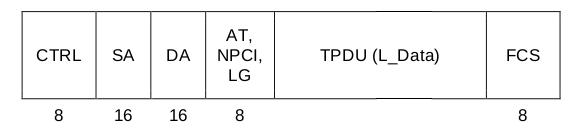
\includegraphics[width=0.8\textwidth]{figures/standardframe}
    \caption{Standard Frame}
    \label{fig:stdframe}
\end{figure}

\begin{figure}
    \centering
    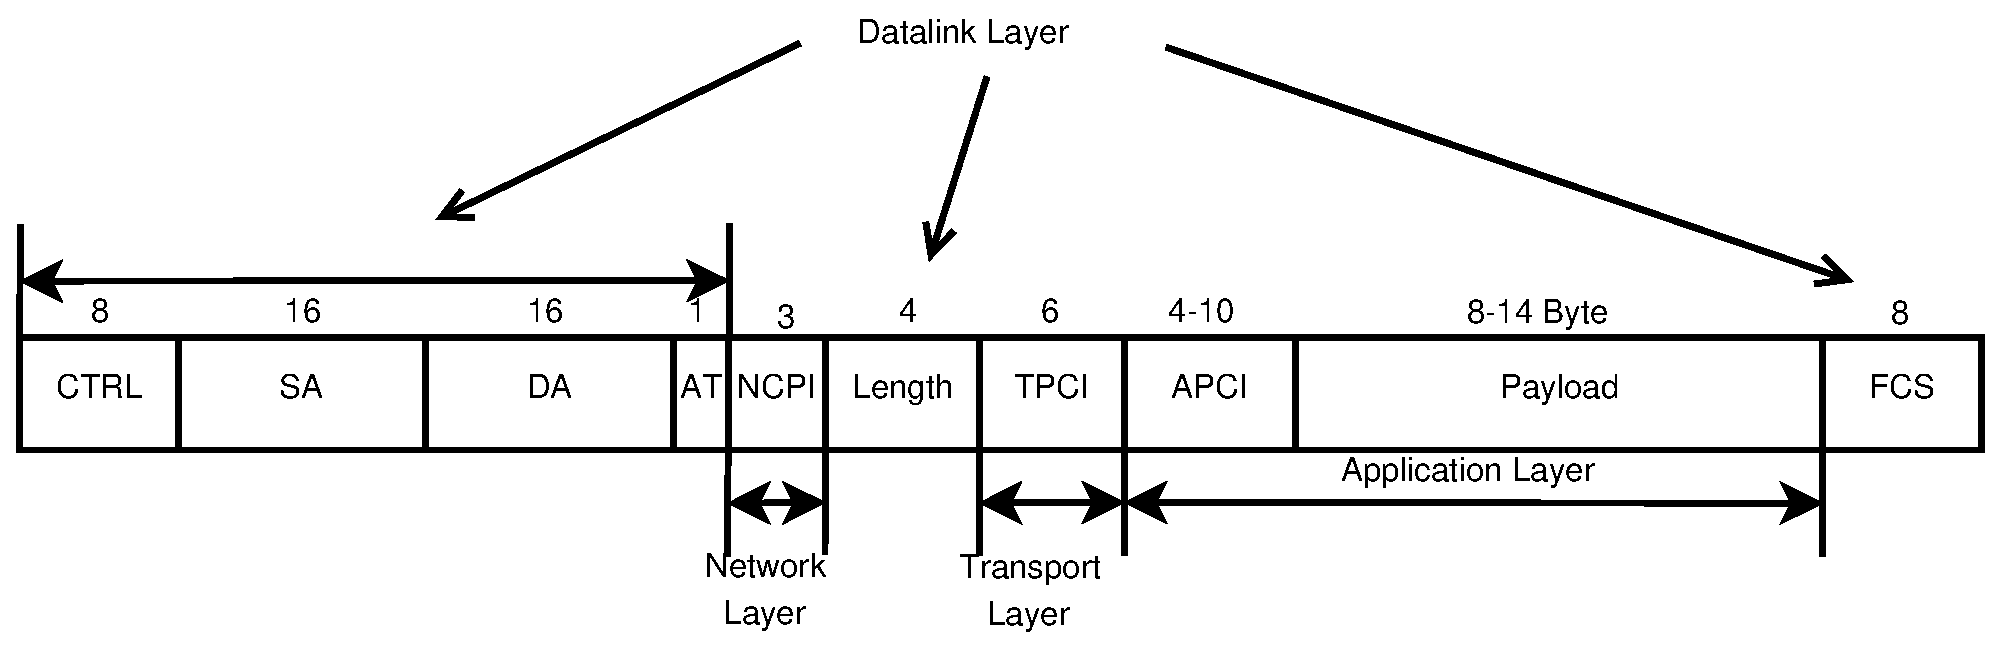
\includegraphics[width=0.8\textwidth]{figures/standardFrame.eps}
    \caption{Standard Frame, in detail}
    \label{fig:stdFrameDetail}
\end{figure}


\subsubsection{Extended L\_Data\_Frame}

The extended frame starts with a control field, as a standard frame. After that, a special \gls{ctrle} follows, as shown in Figure \ref{fig:ctrle}.
Source- and destination addresses, each 2 bytes, follow. To allow the bigger payload, the next byte is used as length field, with the value 0xFF reserved
as escape code, resulting in a maximum payload of 254 byte. After the length field, the payload and the check byte, as defined above, follow.

\begin{figure}
    \centering
    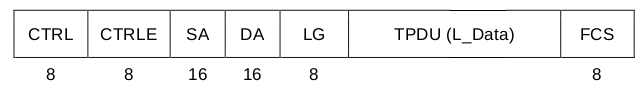
\includegraphics[width=0.8\textwidth]{figures/extendedframe}
    \caption{Extended Frame}
    \label{fig:extframe}
\end{figure}

\begin{figure}
    \centering
    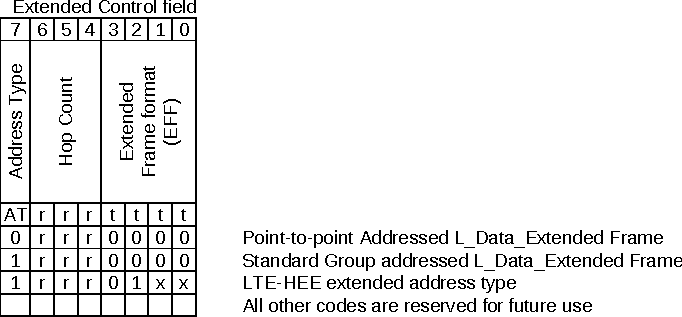
\includegraphics[width=0.8\textwidth]{figures/CTRLE}
    \caption{Extended Frame CTRLE field}
    \label{fig:ctrle}
\end{figure}

\subsubsection{L\_Poll\_Data frame}\label{sec:pollDataFrame}

These frames serve as data requests of the poll-data master for a maximum of 15 bytes
and start with a control field, as defined, followed by the 2 byte source address
of the sender (called Poll\_Data Master). The following 2 byte destination address is 
used to address up to 15 poll slaves, all belonging to the same poll group. The number of
exptected bytes and the check octet follow.
\\
Poll requests are answered by poll slaves by transmitting the databytes in the corresponding poll slave slot.
This is achieved by defining exact timings when each poll data slave must send the requested data. Therefore, such frames can only be used within
one physical segment \cite{knxTP1}.

\subsubsection{Acknowledge frame}\label{sec:ackFrame}

This frames are used to acknowledge the reception of a \gls{knx} data frames for \glspl{ga} or \glspl{ia} and consist
of one byte, sent after a fixed timespan after reception of the frame.

\subsection{KNX addressing scheme}

Two different kinds of addresses are defined: \glspl{ga} or \glspl{ia}, which type is used is determined by the 'address type' flag in the
control field of the datagram(0 = \gls{ia}). While the source address always is an \glspl{ia} and must be unique
within the network, the destination address can be of type group or individual (see Figure \ref{fig:knxAddr} for the layout).
\\
\\
For poll-data frames, the destination address determines the poll group address which must be unique within the physical segment.
\\
\\
Poll data responses as well as acknowledgement frames each just contain 1 byte, i.e., they do not possess source- and destination addresses.

\begin{figure}
 \centering
    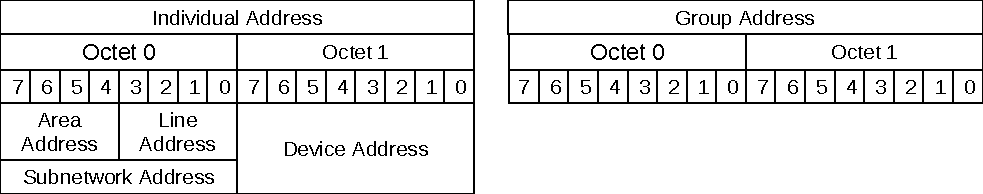
\includegraphics[width=0.9\textwidth]{figures/addresses}
 \caption{\gls{knx} individual and group addresses} 
\label{fig:knxAddr}
%% \subfloat[b]{0.3\textwidth}            
\end{figure}


\subsection{Network layer}

The main task of the network layer is the routing and forwarding of packets, so the main parameter on this layer is the destination address of the
datagram. Additionally, \gls{knx} reserves 3 bits of every standard- and extended data frame as
hop count. This counter is decremented by every router and the frame is discarded if the counter reaches the value zero. This mechanism, known from
\gls{ipv4} \cite{rfc791} \footnote{Originally, this was called \gls{ttl}}, avoids the infinite circulation of packages within an incorrectly configured network.

\subsection{Transport layer}\label{sec:knxTransportLayer}

Accoriding to the \gls{osi} modell, this layer provides point-to-point communication for hosts.
\\
In \gls{knx}, the connection orientated, reliable point-to-point communication mode addresses the \gls{ia} of a remote device and uses a timer to detect timeouts.
Up to to 3 retransmissions are allowed if the sent datagram is not acknowledged. A simple handshake - similar to \gls{tcp} - is used, as shown in Figure \ref{fig:handshake}.
\\
\\
All other modes are unreliable, i.e., unacknowledged, transport mechanisms and can be used to address a \gls{ia}, a \gls{ga} or all devices in the
network. For the latter mode, the special \gls{knx} broadcast address 0x0000 is reserved. 
The \gls{tpci}, included in the control field, determines the type of the \gls{tpdu} and also posseses a 4 bit sequence number by which duplicate datagrams, caused by damaged 
acknowledge-frames, can be discarded.

 \begin{figure}
    \centering
    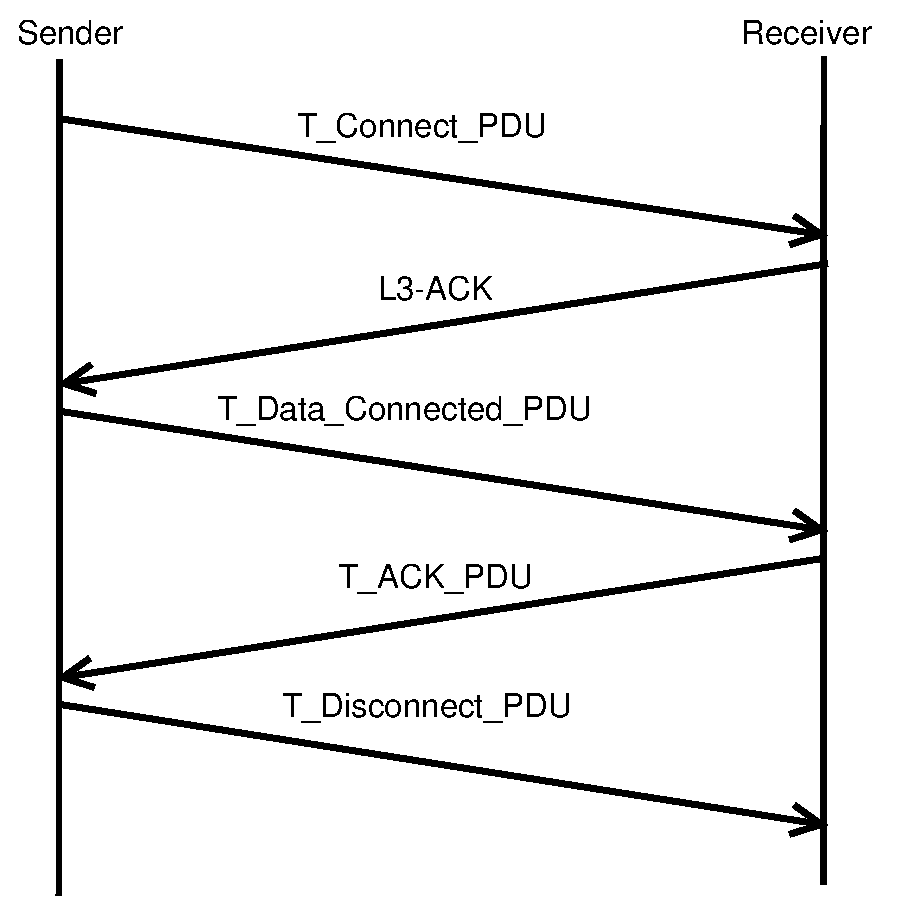
\includegraphics[width=0.5\textwidth]{figures/TransportHandshake.eps}
    \caption{Handshake for connection-orientated communication}
    \label{fig:handshake}
\end{figure}
 
\begin{figure}
    \centering
    \includegraphics[width=0.8\textwidth]{figures/"transport flags".png}
    \caption{Flags used at the Transport Layer}
    \label{fig:tFlags}
\end{figure}
%FIXME: quellenangabe bild, KNX standard

\subsection{Session layer}

This layer is responsible for maintaining sessions, i.e., it provides services to maintain synchronized data exchange. It does not exist in \gls{knx}.

\subsection{Presentation layer}

This layer allows a system-independent data representation, which is not necessary in \gls{knx} because the usage of standardized \glspl{dt}.

\subsection{Application layer}

This layer provides services for process-to-process information through a \gls{knx} network. Up to 10 bits are reserved in the application control field,
inside the \gls{apdu}, containing the application layer service code. The provided services range from tasks like reading or writing group values, distribution of network
parameters to obtaining device information.

%\section{Security in \gls{hbas}}\label{hbaSec}
\glspl{hbas} emerged from automation systems, originally used for building control, summarized as \gls{hvac}.
Central building management, leading to \textit{intelligent buildings}, promises
reduced maintenance costs, energy savings and improved user comfort \cite{1435745}, compensating the initially higher investment costs of such buildings.
Following these arguments it would be natural to integrate additional building management functions like alarm systems, access control or communication systems,
exploiting already existing infrastructure like cabling and thus benefiting from synergy effects.
\\
This trend was contradicted by the fact that in the early days of \gls{hbas}, communication security was not considered a critical requirement:
firstly, the communication was done over wires,
i.e. physical access to the network would have been necessary for attacking the network \cite{knxSpec}. Secondly, the possible threats by misusing \gls{hvac} applications
were considered negligible. Additionally, the devices used in such networks were characterized by very limited processing power - thus, the comprehensive
use of cryptographic measurements would have put remarkable computing loads onto these devices and was therefore considered impracticable.
\\
Today the necessary processing power is available even on embedded systems, meanwhile systems integration continued until a point where security concerns could
no longer be neglected. Therefor, the needs of \gls{hbas} regarding security is introduced next.
\\
\\
Communication networks for \gls{hbas} systems are usually built upon a two-tier model.
\\
FIXME: not finished yet.
	% moved content to chap 1 / problem statement
\section{KNX security concept}
As shown in section \ref{hbaSec}, a paradigm shift towards towards increased security in \gls{hbas} can be observed. 
Despite that fact, the basic \gls{knx} standard does not specify any security mechanisms for control information:
\\

\textit{"For KNX, security is a minor concern, as any breach of security requires local access to the network. 
In the case of KNX TP1 or KNX PL110 networks this requires even physical access to the network wires,
which in nearly all cases is impossible as the wires are inside a building or buried underground.
Hence, security aspects are less of a concern for KNX field level media."} \cite{knxSpec}
\\
\\
For \gls{knx}/\gls{ip}, the physical containment arguments do not apply. To counter this, it is proposed to use firewalls and \glspl{vpn} to prevent unauthorized access,
as well as hiding critical network parameters from public. The latter concept is also known as \textit{"security by obscurity"}, offering - if at all - only 
little protection.
\\
For management communication, a rudimentary, password-based control is used. Therefore, \gls{knx} suffers the following security flaws 
\cite{Granzer05securityin}: for management, the 
used keys are transmitted as cleartext, enabling an attacker to perform a passive attack to obtain the password. Subsequently, the attacker can mount an active
attack, injecting
arbitrary management messages. No methods are foreseen for generation or distribution of the keys.
For control information, an adversary can directly inject arbitrary messages to control the network, allowing passive and active attacks too.
These shortcomings clearly disqualified \gls{knx} for usage in critical environments, restricting its possible field of application.
\\
Today, \gls{hbas} systems are used on a large scale, and the available processing power on embedded computing platforms has risen significantly, so the deployment
of such systems would be possible also in critical environments, under the condition that proper security mechanisms are deployed. For \gls{knx}, several extensions
exist which will be introduced in the next sections.

\subsection{KNX Data Security}

In 2013, the KNX association published "Application Note 158" \cite{knx_data_sec} which specifies the \gls{knx} \gls{s-al}, providing
authentication and encryption, and the \gls{ail}, implementing access control, booth being part of the application layer.
The settlement of these functions above the transport layer allows a transparent, communication media independent end-to-end encryption.

The application layer service code 0xF31 is reserved for this purpose, indicating that a secure header and a \gls{s-al} \gls{pdu} 
follow instead of a plaintext-\gls{pdu}. This allows the flexible usage of the secure services just in situations where they are needed - otherwise, the plaintext application
layer services can be used.

The \gls{s-al} services defines modes for authenticated encryption or authentication-only of a higher-level cleartext \gls{apdu}. As underlying block cipher
\gls{aes}128 is used in \gls{ccm} mode, encrypting the payload with \gls{ctr} and providing integrity with \gls{cbc} mode. The overhead introduced by the 
\gls{mac2} is reduced by 
using only the 32 most significant bits instead of the whole 128 bit block obtained from \gls{cbc}. Source- and destination address as well as
frame- and addresstype, the \gls{tpci}, length information and a 6 byte sequence number determine the \gls{iv} for the \gls{cbc} algorithm and are therefor also protected by the \gls{mac2}.
The sequence number is a simple counter value that provides data freshness, thus preventing replay attacks, and is sent along with every \gls{s-al} \gls{pdu}.
For synchronization of this sequence number between two devices, a \gls{s-al} s	ync-service is defined. Because no sequence number can be used here to guarantee
data freshness, a challenge-response mechanism is used instead.
Two different types of keys are used: a \gls{fdsk} is used for initial setup with the \gls{ets}. The \gls{ets} then generates the \gls{tk}, which is used by the
device for securing of the outgoing messages. Consequently, every device must know the \gls{tk} of it's communication partners.

While the \gls{s-al} empowers two devices to communicate in a secure way, the \gls{ail} allows a fine-grained control which sender has access to which
data objects. Therefore, every \textit{link} (a combination of source address and data or service object) is connected with a \textit{role}, which in turn
has some specific \textit{permissions}. 

\subsection{EIBsec}

EIBsec is another extension to \gls{knx}, providing data integrity, confidentiality and freshness, allowing its deployment in security-critical environments.
A semi-centralized approach is taken here by using special key servers, responsible for dedicated sets
of keys, providing a sophisticated key management. EIBsec divides a \gls{knx} network into subnets, connected by devices called \gls{acu}. Beside their native
task, i.e. routing traffic, they
 are responsible for the key management of their network segments, which includes key generation, distribution and revocation. Every standard device that
 wishes to communicate with other devices must at first retrieve the corresponding secret key from its responsible \gls{acu}, which can therefor control the
 group membership of the requesting device by allowing or denying the request respectively by revoking the key at a later point in time.

EIBsec uses two different keys: in normal mode, a session with the keyserver is established to retrieve the session key, establishing a secure channel.
This mode uses encryption-only by utilizing a \gls{psk}, integrity must therefor be guaranteed by the sender of the message. Counter mode is used for transmitting management and
group data over the secure channel. A simple \gls{crc} is added to the payload before encryption and shall guarantee integrity. Booth modes encrypt the traffic
on transport level, allowing standard routers to handle the datagrams. As block cipher, \gls{aes}-128 is used in \gls{ctr} mode.

FIXME: zitieren / originalpaper...?

\subsection{KNX IP Security}

This work focuses on securing the \gls{knx} \gls{ip} specification, which can be used as backbone for connecting distinct \gls{knx} installations \cite{5195839}.
Thanks to the widespread use of \gls{tcp}/\gls{ip}, a wide range of physical transport mechanisms can be utilized.
\\
A structure comparable to the design of \gls{tls} is defined by building a distinct security layer, residing above the transport layer (therefore, it directly
connects the transport to the application layer, because session- and presentation layer are empty, as defined by the \gls{knx} specifications, see chapter
\ref{ch:knx}).
\\
The design distinguishes 3 different types of modes: 

in the \textit{configuration phase}, every device that wants to participate in the secure network
generates an asymmetric key pair, which is sent to the \gls{ets} over a secure channel (for example, by transmitting the data over a direct, serial connection
between the \gls{ets} host and the \gls{knx} device).
The \gls{ets}, acting as \gls{ca1}, signs the combination of \gls{ip} and public key with its own private key, thus generating a certificate, which is sent back to the device, along
with the public key of the \gls{ets}. 

After that, the \textit{key set distribution phase} starts, where a unicast and a multicast scenario are differentiated:
in the unicast case, the device initiating the communication - called client - obtains the key set from the target device by a 2-step handshake: at first, mutual entity 
authenticity is established by utilizing the certificate provided by the \gls{ets}. Afterwards the keyset is obtained from the target, which concludes the second
phase.

In the last step, secure communication can take place, i.e. the the client is able to
encrypt the data with the obtained key and sends it to the target device.

For the multicast scenario, a distinct \textit{coordinator}, responsible for maintaining the group key, is necessary. Every powered-up device
identifies the coordinator as soon as possible by broadcasting \textit{hello} requests, adopting the coordinator role if no replies are received in time.
To actually send a payload, the group key is obtained from the coordinator and the data is sent to the group, analog to the unicast case.
By adding mechanisms to detect "dead" coordinators and delegating the coordinator role to a different device, the design avoids a \gls{spof}.


\section{Summary}
Examining the security measurements shows up parallels to the \gls{ipv4} world. As with \gls{knx}, no security measurements were foreseen in the
original standard. The problem was
fixed here in two ways: \gls{tls} was added as a sublayer between \gls{osi} layers 4 and 5, allowing application-transparent encryption and authentication, 
similar to KNX Application Note 158, as described above. The second solution was the introduction of \gls{ipsec}, extending \gls{ipv4} and thus enabling authentication and encryption on \gls{ip} level.
\\
\\
Despite the \gls{knx} extensions, no solution providing high availability exists. Therefore, this work proposes to combination of cryptographic measurements with
redundancy mechanisms, allowing its deployment in more demanding environments.

%%%%%%%%%%%%%%%%%%%%%%%%%%%%%%%%%%%%%%%%%

%%%%%%%%%%%%%%%%%%%%%%%%%%%%%%%%%%%%%%%%%
\chapter{Concept}
\label{ch:concept}
\section{Basic Assumptions}

The aim of this work is to propose a \gls{knx} prototype, applicable for environments with increased availability demands.
The prototype should be designed in a transparent way, utilizing a "plug and play" functionality to build a secure \gls{knx} network.
This means that a device outside of this network, unaware of
the secured \gls{knx} network, should be able to deliver through and receive messages from such a secured network without any prerequisites. 
Every device with one connection to an unsecured \gls{knx} network (called cleartext \gls{knx} line) and two distinct connections to a secured \gls{knx}
network (called secure lines, running the master daemon, will work
as a security gateway. Thus, the presence of at least 2 of these security gateways connected to each other by two secure lines will constitute a 
secured \gls{knx} area, bridging between areas with increased security demands, as shown in figure \ref{fig:secArea}.
\\
\\
The basic tasks of such security gateways consist of:
\begin{itemize}
 \item establishing keys with it's communication partners within the secured \gls{knx} network (the security gateways)
% \item maintaining some kind of synchronization token between all security gateways
 \item providing redundant communication lines, achieving improved availability by encrypting and authenticating all messages which are received on the unsecured line, and delivering them to the proper security gateways which act as
 border device for the given group address, using booth secure lines
 \item checking all messages which are received on the secured lines for integrity and authenticity, removing duplicates, unwrapping and delivering them to
 the unsecured area
\end{itemize}

\subsection{Security Related Architectural Overview}

As stated in chapter \ref{ch:knx}, 3 different possibilities for communication within a \gls{knx} network are possible: point to point, multicast and broadcast.
To introduce as little additional traffic into the network as possible, a sound concept for translating clear- to secure-\gls{knx} address (and vice versa) has to
be defined. While in principle it would be possible to use the communication modes in a transparent way (i.e., point-to-point in unsecured \gls{knx} translates
to point-to-point in secured \gls{knx}, and vice versa, and so on), this approach leads to some serious problems, rendering this solution impracticable:
due to the topology of \gls{knx}, it is impossible to know a priori the exact physical location of a device (i.e., its \gls{ia}). Additionally,
every device can be member of an arbitrary number of group addresses (bounded by the maximum number of group addresses), which also is not known in advance.
Group-membership is also subject to change and therefore complicates the situation. Finally, devices can leave or join the network at every moment by powering the
device up or down.
\\
Therefore, a device which receives a message on its unsecured \gls{knx} line, examining the destination address, simply does
not know which device(s), if any, will be the gateway(s) responsible for delivering this datagram one hop toward its final destination,
regardless if the destination address is a \glspl{ia} or a \gls{ga}.
\begin{figure}
    \centering
    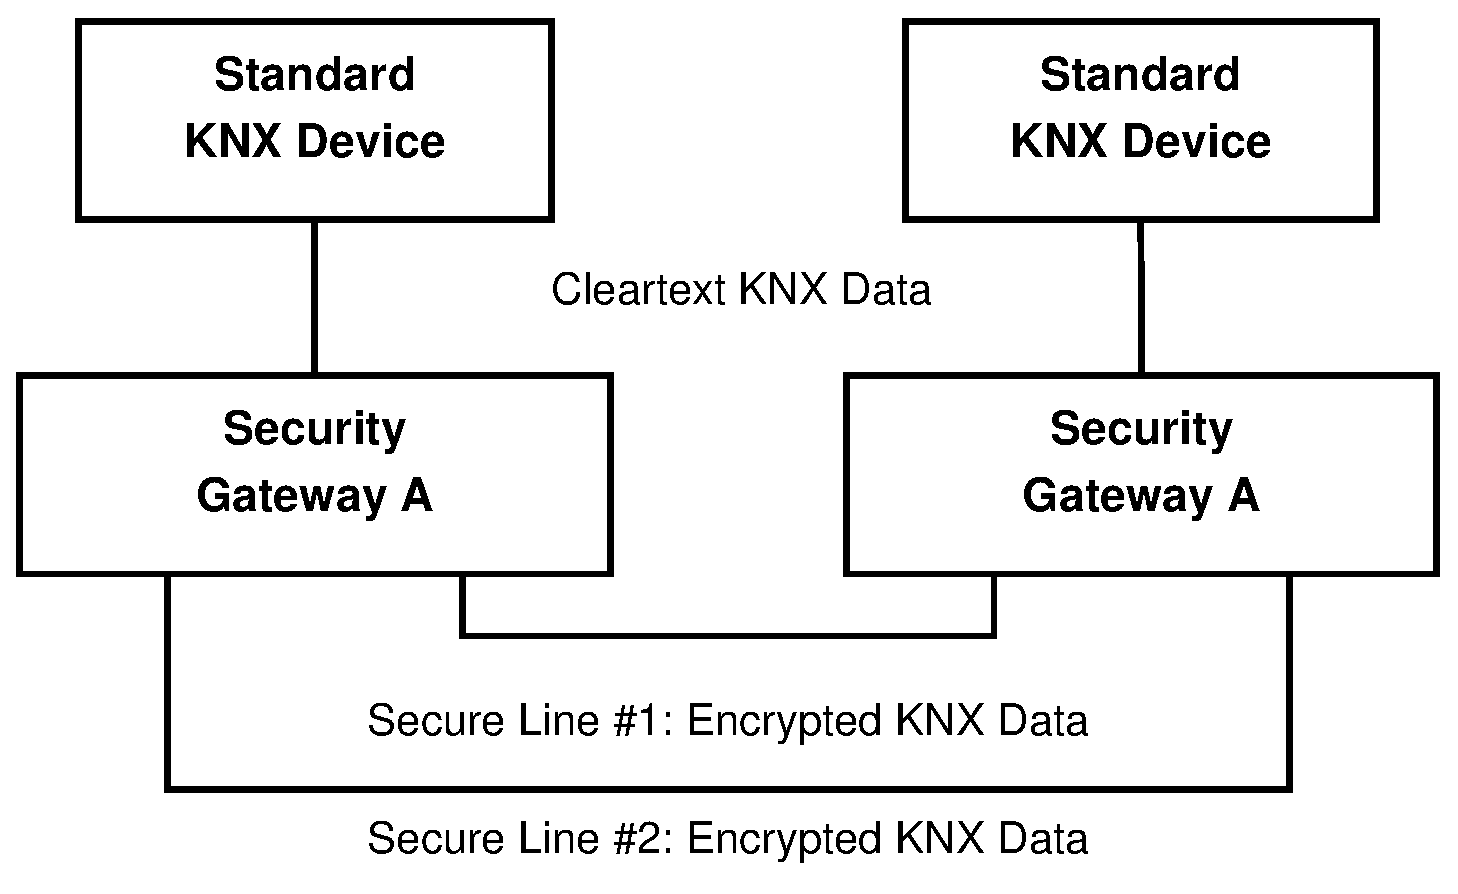
\includegraphics[width=1\textwidth]{figures/SecureArea.eps}
    \caption{Secure Area}
    \label{fig:secArea}
\end{figure}
\\
\\
A straightforward solution to this problem would be to wrap every datagram which enters the secured \gls{knx} network via a security gateway into a new, properly secured
broadcast datagram, and delivering this new package to the secured \gls{knx} network. Then, the package would be available to all other security gateways, which
will unwrap it and forward the resulting inner datagram to its unsecured \gls{knx} line. If the destination address (group or individual) of the actual payload
is assigned to a device connected
to the unsecured \gls{knx} network, the device holding this \gls{ia} or \gls{ga} will recognize it and the package will reach its destination. 
Otherwise it will simply be discarded.
\\
A serious constraint rising from this broadcast approach is that a single,
global network key must be used, because every security gateway must be able to decrypt and check every package which it receives on it's secured lines,
even if it does not serve as gateway to the wanted group address. 
The key of course can be renegotiated among the security gateways at every time, but this approach is considered
unsafe because an attacker can target \textit{any} of the security gateways constituting the secure network. An adversary breaking one single device gains
access to the network traffic of all devices. This could be achieved by physical access to any of the security gateways, for example by reading out the
memory of the device, and thus obtaining the globally used network key. This way, the network traffic can be decrypted by the adversary as long as no new
key is renegotiated. Another problem is that multi-party key negotiation is a costly task if a public-private key scheme
is to be used: as shown in figures \ref{fig:dh1} and \ref{fig:dh2}, a lot of messages have to be exchanged before actual an encryption can be done. 
\\
\\
To encounter this problems, different keys must be used, thus achieving pairwise end-to-end encryption between all devices. 
%This way it is also possible to achieve different security levels, depending on the function a 
%particular unsecured \gls{knx} device fulfills. It would be possible, for example, to distinguish between 'normal' gateways and 'hardened'
%gateways which are specially guarded against physical access, for example by applying physical intrusion detection. Thus,
%the risk of breaking the whole system is reduced, because breaking a device in one security level does not affect the security of the devices with other
%security levels.
%So, for breaking all $n$ security levels of a system, at least $n$ devices, all belonging to different levels must be broken.
%As a motivating example, imagine a setup which consists of window controls in an upper floor, and door controls in the
%base level. Obviously, the security constraints for the latter one would be higher. By using normal devices for window control, and hardened devices for
%door control, a security firewall can be deployed, thus containing the damage an adversary can do to the whole system.
Figure \ref{fig:firewall} shows the logical connections within an \gls{knx} network using end-to-end encryption. An 
attack of node $A$ can only compromise keys known to the device, thus effectively separating communication between the nodes $B$, $C$, and $D$ from
the attacker. 
\begin{figure}
  \centering
    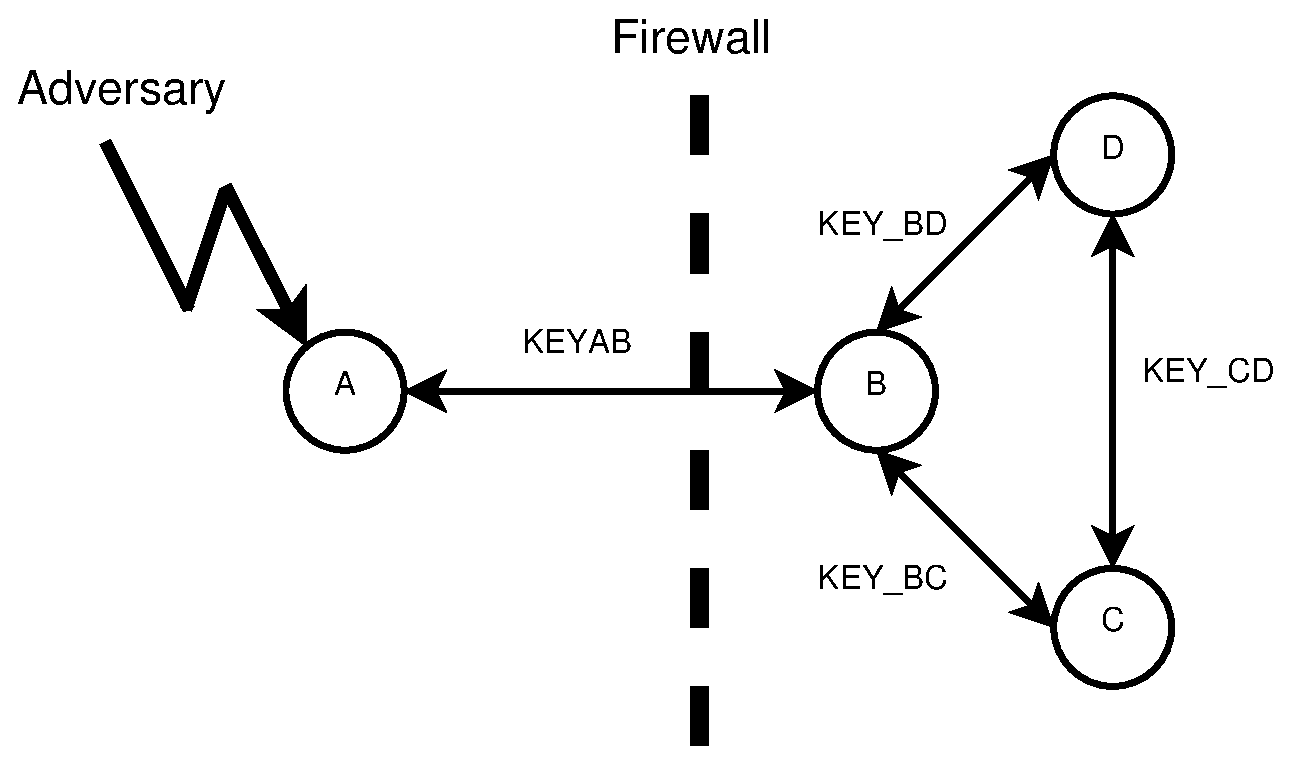
\includegraphics[width=0.8\textwidth]{figures/firewall2.eps}
% % Graphic for TeX using PGF
% Title: /home/hglanzer/ownCloud/Diplomarbeit/MasterThesisTemplate/figures/firewall.dia
% Creator: Dia v0.97.2
% CreationDate: Fri Dec  5 19:14:47 2014
% For: hglanzer
% \usepackage{tikz}
% The following commands are not supported in PSTricks at present
% We define them conditionally, so when they are implemented,
% this pgf file will use them.
\ifx\du\undefined
  \newlength{\du}
\fi
\setlength{\du}{15\unitlength}
\begin{tikzpicture}
\pgftransformxscale{1.000000}
\pgftransformyscale{-1.000000}
\definecolor{dialinecolor}{rgb}{0.000000, 0.000000, 0.000000}
\pgfsetstrokecolor{dialinecolor}
\definecolor{dialinecolor}{rgb}{1.000000, 1.000000, 1.000000}
\pgfsetfillcolor{dialinecolor}
\pgfsetlinewidth{0.100000\du}
\pgfsetdash{}{0pt}
\pgfsetdash{}{0pt}
\pgfsetbuttcap
\pgfsetmiterjoin
\pgfsetlinewidth{0.100000\du}
\pgfsetbuttcap
\pgfsetmiterjoin
\pgfsetdash{}{0pt}
\definecolor{dialinecolor}{rgb}{1.000000, 1.000000, 1.000000}
\pgfsetfillcolor{dialinecolor}
\pgfpathellipse{\pgfpoint{12.000000\du}{5.000000\du}}{\pgfpoint{1.000000\du}{0\du}}{\pgfpoint{0\du}{1.000000\du}}
\pgfusepath{fill}
\definecolor{dialinecolor}{rgb}{0.000000, 0.000000, 0.000000}
\pgfsetstrokecolor{dialinecolor}
\pgfpathellipse{\pgfpoint{12.000000\du}{5.000000\du}}{\pgfpoint{1.000000\du}{0\du}}{\pgfpoint{0\du}{1.000000\du}}
\pgfusepath{stroke}
\pgfsetbuttcap
\pgfsetmiterjoin
\pgfsetdash{}{0pt}
\definecolor{dialinecolor}{rgb}{0.000000, 0.000000, 0.000000}
\pgfsetstrokecolor{dialinecolor}
\pgfpathellipse{\pgfpoint{12.000000\du}{5.000000\du}}{\pgfpoint{1.000000\du}{0\du}}{\pgfpoint{0\du}{1.000000\du}}
\pgfusepath{stroke}
\pgfsetlinewidth{0.100000\du}
\pgfsetdash{}{0pt}
\pgfsetdash{}{0pt}
\pgfsetbuttcap
\pgfsetmiterjoin
\pgfsetlinewidth{0.100000\du}
\pgfsetbuttcap
\pgfsetmiterjoin
\pgfsetdash{}{0pt}
\definecolor{dialinecolor}{rgb}{1.000000, 1.000000, 1.000000}
\pgfsetfillcolor{dialinecolor}
\pgfpathellipse{\pgfpoint{18.000000\du}{1.000000\du}}{\pgfpoint{1.000000\du}{0\du}}{\pgfpoint{0\du}{1.000000\du}}
\pgfusepath{fill}
\definecolor{dialinecolor}{rgb}{0.000000, 0.000000, 0.000000}
\pgfsetstrokecolor{dialinecolor}
\pgfpathellipse{\pgfpoint{18.000000\du}{1.000000\du}}{\pgfpoint{1.000000\du}{0\du}}{\pgfpoint{0\du}{1.000000\du}}
\pgfusepath{stroke}
\pgfsetbuttcap
\pgfsetmiterjoin
\pgfsetdash{}{0pt}
\definecolor{dialinecolor}{rgb}{0.000000, 0.000000, 0.000000}
\pgfsetstrokecolor{dialinecolor}
\pgfpathellipse{\pgfpoint{18.000000\du}{1.000000\du}}{\pgfpoint{1.000000\du}{0\du}}{\pgfpoint{0\du}{1.000000\du}}
\pgfusepath{stroke}
\pgfsetlinewidth{0.100000\du}
\pgfsetdash{}{0pt}
\pgfsetdash{}{0pt}
\pgfsetbuttcap
\pgfsetmiterjoin
\pgfsetlinewidth{0.100000\du}
\pgfsetbuttcap
\pgfsetmiterjoin
\pgfsetdash{}{0pt}
\definecolor{dialinecolor}{rgb}{1.000000, 1.000000, 1.000000}
\pgfsetfillcolor{dialinecolor}
\pgfpathellipse{\pgfpoint{18.000000\du}{9.000000\du}}{\pgfpoint{1.000000\du}{0\du}}{\pgfpoint{0\du}{1.000000\du}}
\pgfusepath{fill}
\definecolor{dialinecolor}{rgb}{0.000000, 0.000000, 0.000000}
\pgfsetstrokecolor{dialinecolor}
\pgfpathellipse{\pgfpoint{18.000000\du}{9.000000\du}}{\pgfpoint{1.000000\du}{0\du}}{\pgfpoint{0\du}{1.000000\du}}
\pgfusepath{stroke}
\pgfsetbuttcap
\pgfsetmiterjoin
\pgfsetdash{}{0pt}
\definecolor{dialinecolor}{rgb}{0.000000, 0.000000, 0.000000}
\pgfsetstrokecolor{dialinecolor}
\pgfpathellipse{\pgfpoint{18.000000\du}{9.000000\du}}{\pgfpoint{1.000000\du}{0\du}}{\pgfpoint{0\du}{1.000000\du}}
\pgfusepath{stroke}
\pgfsetlinewidth{0.100000\du}
\pgfsetdash{}{0pt}
\pgfsetdash{}{0pt}
\pgfsetbuttcap
\pgfsetmiterjoin
\pgfsetlinewidth{0.100000\du}
\pgfsetbuttcap
\pgfsetmiterjoin
\pgfsetdash{}{0pt}
\definecolor{dialinecolor}{rgb}{1.000000, 1.000000, 1.000000}
\pgfsetfillcolor{dialinecolor}
\pgfpathellipse{\pgfpoint{24.000000\du}{5.000000\du}}{\pgfpoint{1.000000\du}{0\du}}{\pgfpoint{0\du}{1.000000\du}}
\pgfusepath{fill}
\definecolor{dialinecolor}{rgb}{0.000000, 0.000000, 0.000000}
\pgfsetstrokecolor{dialinecolor}
\pgfpathellipse{\pgfpoint{24.000000\du}{5.000000\du}}{\pgfpoint{1.000000\du}{0\du}}{\pgfpoint{0\du}{1.000000\du}}
\pgfusepath{stroke}
\pgfsetbuttcap
\pgfsetmiterjoin
\pgfsetdash{}{0pt}
\definecolor{dialinecolor}{rgb}{0.000000, 0.000000, 0.000000}
\pgfsetstrokecolor{dialinecolor}
\pgfpathellipse{\pgfpoint{24.000000\du}{5.000000\du}}{\pgfpoint{1.000000\du}{0\du}}{\pgfpoint{0\du}{1.000000\du}}
\pgfusepath{stroke}
\pgfsetlinewidth{0.100000\du}
\pgfsetdash{}{0pt}
\pgfsetdash{}{0pt}
\pgfsetbuttcap
{
\definecolor{dialinecolor}{rgb}{0.000000, 0.000000, 0.000000}
\pgfsetfillcolor{dialinecolor}
% was here!!!
\pgfsetarrowsstart{stealth}
\pgfsetarrowsend{stealth}
\definecolor{dialinecolor}{rgb}{0.000000, 0.000000, 0.000000}
\pgfsetstrokecolor{dialinecolor}
\draw (17.000000\du,1.000000\du)--(12.000000\du,4.000000\du);
}
\pgfsetlinewidth{0.100000\du}
\pgfsetdash{}{0pt}
\pgfsetdash{}{0pt}
\pgfsetbuttcap
{
\definecolor{dialinecolor}{rgb}{0.000000, 0.000000, 0.000000}
\pgfsetfillcolor{dialinecolor}
% was here!!!
\pgfsetarrowsstart{stealth}
\pgfsetarrowsend{stealth}
\definecolor{dialinecolor}{rgb}{0.000000, 0.000000, 0.000000}
\pgfsetstrokecolor{dialinecolor}
\draw (12.000000\du,6.000000\du)--(17.000000\du,9.000000\du);
}
\pgfsetlinewidth{0.100000\du}
\pgfsetdash{}{0pt}
\pgfsetdash{}{0pt}
\pgfsetbuttcap
{
\definecolor{dialinecolor}{rgb}{0.000000, 0.000000, 0.000000}
\pgfsetfillcolor{dialinecolor}
% was here!!!
\pgfsetarrowsstart{stealth}
\pgfsetarrowsend{stealth}
\definecolor{dialinecolor}{rgb}{0.000000, 0.000000, 0.000000}
\pgfsetstrokecolor{dialinecolor}
\draw (19.000000\du,9.000000\du)--(24.000000\du,6.000000\du);
}
\pgfsetlinewidth{0.100000\du}
\pgfsetdash{}{0pt}
\pgfsetdash{}{0pt}
\pgfsetbuttcap
{
\definecolor{dialinecolor}{rgb}{0.000000, 0.000000, 0.000000}
\pgfsetfillcolor{dialinecolor}
% was here!!!
\pgfsetarrowsstart{stealth}
\pgfsetarrowsend{stealth}
\definecolor{dialinecolor}{rgb}{0.000000, 0.000000, 0.000000}
\pgfsetstrokecolor{dialinecolor}
\draw (19.000000\du,1.000000\du)--(24.000000\du,4.000000\du);
}
\pgfsetlinewidth{0.100000\du}
\pgfsetdash{}{0pt}
\pgfsetdash{}{0pt}
\pgfsetbuttcap
{
\definecolor{dialinecolor}{rgb}{0.000000, 0.000000, 0.000000}
\pgfsetfillcolor{dialinecolor}
% was here!!!
\pgfsetarrowsstart{stealth}
\pgfsetarrowsend{stealth}
\definecolor{dialinecolor}{rgb}{0.000000, 0.000000, 0.000000}
\pgfsetstrokecolor{dialinecolor}
\draw (18.000000\du,2.000000\du)--(18.000000\du,8.000000\du);
}
\pgfsetlinewidth{0.300000\du}
\pgfsetdash{{1.000000\du}{1.000000\du}}{0\du}
\pgfsetdash{{1.000000\du}{1.000000\du}}{0\du}
\pgfsetbuttcap
{
\definecolor{dialinecolor}{rgb}{0.000000, 0.000000, 0.000000}
\pgfsetfillcolor{dialinecolor}
% was here!!!
\definecolor{dialinecolor}{rgb}{0.000000, 0.000000, 0.000000}
\pgfsetstrokecolor{dialinecolor}
\draw (15.707107\du,-1.388909\du)--(15.707107\du,11.611091\du);
}
% setfont left to latex
\definecolor{dialinecolor}{rgb}{0.000000, 0.000000, 0.000000}
\pgfsetstrokecolor{dialinecolor}
\node[anchor=west] at (18.292893\du,5.000000\du){$Key_{BC}$};
% setfont left to latex
\definecolor{dialinecolor}{rgb}{0.000000, 0.000000, 0.000000}
\pgfsetstrokecolor{dialinecolor}
\node[anchor=west] at (11.469670\du,4.893934\du){A};
% setfont left to latex
\definecolor{dialinecolor}{rgb}{0.000000, 0.000000, 0.000000}
\pgfsetstrokecolor{dialinecolor}
\node[anchor=west] at (17.505025\du,1.000000\du){B};
% setfont left to latex
\definecolor{dialinecolor}{rgb}{0.000000, 0.000000, 0.000000}
\pgfsetstrokecolor{dialinecolor}
\node[anchor=west] at (17.505025\du,9.000000\du){C};
% setfont left to latex
\definecolor{dialinecolor}{rgb}{0.000000, 0.000000, 0.000000}
\pgfsetstrokecolor{dialinecolor}
\node[anchor=west] at (23.505025\du,5.000000\du){D};
% setfont left to latex
\definecolor{dialinecolor}{rgb}{0.000000, 0.000000, 0.000000}
\pgfsetstrokecolor{dialinecolor}
\node[anchor=west] at (12.000000\du,2.000000\du){$Key_{AB}$};
% setfont left to latex
\definecolor{dialinecolor}{rgb}{0.000000, 0.000000, 0.000000}
\pgfsetstrokecolor{dialinecolor}
\node[anchor=west] at (12.000000\du,9.000000\du){$Key_{AC}$};
% setfont left to latex
\definecolor{dialinecolor}{rgb}{0.000000, 0.000000, 0.000000}
\pgfsetstrokecolor{dialinecolor}
\node[anchor=west] at (22.000000\du,2.000000\du){$Key_{BD}$};
% setfont left to latex
\definecolor{dialinecolor}{rgb}{0.000000, 0.000000, 0.000000}
\pgfsetstrokecolor{dialinecolor}
\node[anchor=west] at (22.000000\du,9.000000\du){$Key_{CD}$};
% setfont left to latex
\definecolor{dialinecolor}{rgb}{0.000000, 0.000000, 0.000000}
\pgfsetstrokecolor{dialinecolor}
\node[anchor=west] at (14.000000\du,9.000000\du){};
\pgfsetlinewidth{0.200000\du}
\pgfsetdash{}{0pt}
\pgfsetdash{}{0pt}
\pgfsetbuttcap
{
\definecolor{dialinecolor}{rgb}{0.000000, 0.000000, 0.000000}
\pgfsetfillcolor{dialinecolor}
% was here!!!
\definecolor{dialinecolor}{rgb}{0.000000, 0.000000, 0.000000}
\pgfsetstrokecolor{dialinecolor}
\draw (7.939094\du,0.782827\du)--(9.353307\du,3.611255\du);
}
\pgfsetlinewidth{0.200000\du}
\pgfsetdash{}{0pt}
\pgfsetdash{}{0pt}
\pgfsetbuttcap
{
\definecolor{dialinecolor}{rgb}{0.000000, 0.000000, 0.000000}
\pgfsetfillcolor{dialinecolor}
% was here!!!
\definecolor{dialinecolor}{rgb}{0.000000, 0.000000, 0.000000}
\pgfsetstrokecolor{dialinecolor}
\draw (9.303307\du,3.611255\du)--(9.975059\du,1.596000\du);
}
\pgfsetlinewidth{0.200000\du}
\pgfsetdash{}{0pt}
\pgfsetdash{}{0pt}
\pgfsetbuttcap
{
\definecolor{dialinecolor}{rgb}{0.000000, 0.000000, 0.000000}
\pgfsetfillcolor{dialinecolor}
% was here!!!
\pgfsetarrowsend{stealth}
\definecolor{dialinecolor}{rgb}{0.000000, 0.000000, 0.000000}
\pgfsetstrokecolor{dialinecolor}
\draw (9.975059\du,1.525290\du)--(11.353917\du,4.247651\du);
}
% setfont left to latex
\definecolor{dialinecolor}{rgb}{0.000000, 0.000000, 0.000000}
\pgfsetstrokecolor{dialinecolor}
\node[anchor=west] at (6.439525\du,0.358563\du){Adversary};
\end{tikzpicture}

 \caption{Firewall}
 \label{fig:firewall}
\end{figure}
As stated above, to be able to use different keys every security gateway has to know how to reach a given address so that the data can be encrypted
exclusively for the responsible gateway. The solution to this problem is to maintain some kind of routing table, mapping \glspl{ga} and \glspl{ia} of unsecured
\gls{knx} devices to \glspl{ia} of responsible security gateways	.
Such a routing table can be built statically at setup time, with the obvious disadvantage
that the exact topology of the to be applied network has to be known in advance, thus reducing the flexibility. Here, every security gateway holds a static 
table which consists of mappings between \glspl{ia} or \glspl{ga} of unsecured \gls{knx} devices and \glspl{ia} of security gateways at the border
between the secured and the unsecured \gls{knx} network, as well as all keys used for the particular security level the gateway belongs to.
This table would be generated once, after the topology of the network has been fixed, and must be equipped with the proper keys and can then
be copied to the security gateways constituting the secured \gls{knx} area. New security gateways can be deployed as long as they only introduce sending 
unsecured \gls{knx} devices, whose recipients are already mapped, known group addresses. A new group address, introduced by a newly installed device behind
an already existing security gateway, will not be reachable, simply because the routing information is not available. 
Another disadvantage is that the deployment of new
security gateways, connecting devices with new or already known \glspl{ga}, is impossible as the \gls{ia} of the new gateway - which of
course must be unique - is unknown to the existing setup, thus making the new unsecured \gls{knx} devices unreachable.
\\
To tackle this problem, another approach would be to build this mapping table dynamically. Therefore, every security gateway must periodically poll
on it's unsecured lines for \gls{knx} devices, thus populating a list of reachable \gls{knx} devices. Whenever a 
device wants to send data to a group address, it has to do a lookup first to obtain the \glspl{ia} of the responsible security gateways: the lookup
must contain the wanted group address, as well as the senders public key.
Every 
gateway which finds the wanted group address in its group list must reply with an according message to the requester, thus announcing that it is responsible
for delivering data to the wanted group address, and must also publish it's own public key, thus allowing pairwise end-to-end encryption.
This procedure requires no a priori knowledge of
the network topology, so security gateways can be added to the network as well as unsecured \gls{knx} devices behind new or existing gateways at any time. This
flexibility of course has to be purchased with increased complexity as well as additional traffic introduced into the network.
\\
\\
A middle course is chosen: the reachable group address list is generated whenever a new security gateway is added to the network,
 handling discovery of this group addresses as described
above. This allows to deploy new security gateways with connected unsecured devices, thus achieving a comprise between flexibility and complexity. 
\\
Sending data to a group address therefor follows the triad discovery request, discovery response and actual data transfer, shown in figure \ref{fig:prot1}. Broadcast
messages are depicted as solid end of the arrow, the rest denoting unicast messages.
\begin{figure}
  \centering
    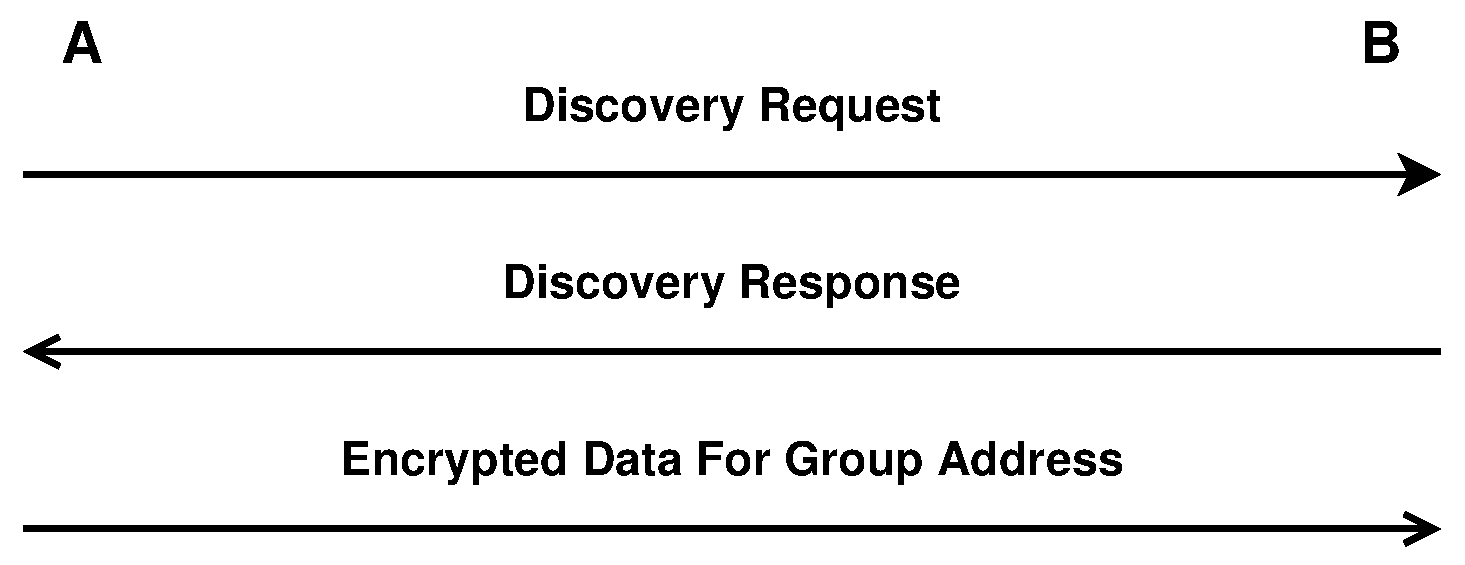
\includegraphics[width=0.8\textwidth]{figures/protokoll1.eps}
 \caption{Communication schema}
 \label{fig:prot1}
\end{figure}
To enable multiple devices to announce responsibility for a group address, the device wanting to transmit data to this group address must accept discovery responses
following it's request message for a short time window.
\\
\\
The discovery messages generated by security gateways should be encrypted too. Although these datagrams don't contain \gls{knx} data per se, they allow
a listening adversary to learn the topology of the network, knowledge which can be valuable for developing an attack strategy, as well as generating meta data.
For example, if an attacker learns that a particular security gateway is responsible for only one group address and further gets knowledge that this 
group address is responsible for switching a light (i.e. by visual observation), the attacker afterwards may be able to derive a personal profile just by seeing
packages for this group address, although the payload of the datagrams to the responsible security gateway are encrypted.
If the discovery messages are encrypted too the adversary doesn't know how many and what
group addresses are behind a specif gateway, and it will be harder to derive personal profiles or to gather knowledge of the network topology.
\\
Discovery request messages must be broadcast messages, readable by all security gateways. To limit the protocol overhead, a global network key is used here.
\\
\\
To provide authenticity, all datagrams passing the secured \gls{knx} network must contain a \gls{mac2} to prevent modification of them.
\\
Defense against replay attacks is achieved by counters.These must be strictly monotonically
increasing and must not overflow. The counters can be compared to an initialization vector that prevents the mapping of same cleartext messages to same ciphertext messages
under the same encryption key.
\\
Two different types of counters are used: one global counter $Ctr_{global}$, used for avoiding replay attacks against discovery messages. A second kind of counter
is used for the actual data transfer. Beside avoiding replay attacks, this counter is necessary to detect and delete duplicates, caused by the redundant network, 
see \ref{ctrAvail} for details.
\\
Usage of the global counter $Ctr_{global}$ raises another question, namely how a new device gets knowledge of the actual value of $Ctr_{global}$.
Therefor, a synchronization service must be defined, allowing a newly powered up device to synchronize with the rest of the network \ref{fig:syncProt}.
\begin{figure}
  \centering
    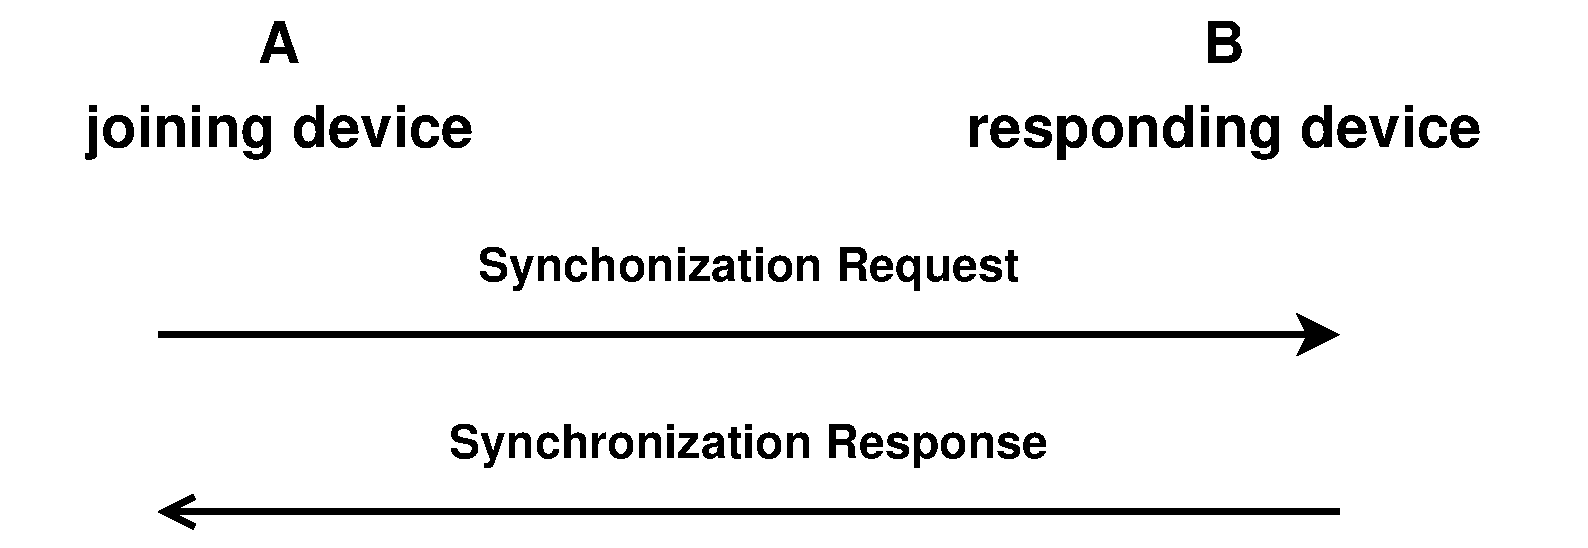
\includegraphics[width=0.8\textwidth]{figures/protSync.eps}
 \caption{Synchronization service}
 \label{fig:syncProt}
\end{figure}
Replay attacks are mitigated by including the actual time into \gls{mac2} calculation. Low temporal resolution relaxes time-synchronization issues between
different devices.

\subsubsection{Key Management}

While it would be possible to use a centralized concept, no trusted on-line party is used in this work. A centralized approach would need fall-back key servers
which inherit the task of generating and distributing keys and parameters in case of a master key server failure. Otherwise, the network would suffer from a
single point of failure in case no such fall-back mechanism is applied, an assumption that would clearly disqualify the design as highly available.
\\
The following keys are used:

\begin{itemize}
 \item A long-term key known to all security gateways is used. As already stated, this key must be copied to every device at setup time. 
This pre-shared key $k_{psk}$ is used for symmetric encryption and serves different purposes: first, it is used to authenticate synchronization messages.
Secondly, this key $k_{psk}$ is used to encrypt discovery requests and discovery responses.
 %\item $k_{global}$ is used to authenticate and encrypt locally generated and decrypt received discovery requests, as well as to authenticate and encrypt
 %locally generated discovery responses and decrypt received ones. These discovery service datagrams securely transport the third type of keys:
 \item Asymmetric keys are used for end-to-end encryption of the actual data packages between 2 security gateways. \gls{ecdh} serves as key negotiation algorithm.
 To protect against man-in-the-middle attacks, authenticity of the \gls{dh} parameters must be assured.
 \item This is the task of the third kind of keys: another pre-shared key is used to authenticate the \gls{dh} parameters.
\end{itemize}


\subsection{Redundancy Related Architectural Overview}\label{ctrAvail}
 
Whenever a \gls{knx} package is
generated by a device on an unsecured line (called client), the connected security gateway will read, duplicate and encapsulate it into another \gls{knx} frame 
and then send over booth lines. If booth lines are available, i.e. there is, for example, no shortcut, the security gateway responsible for forwarding the frame
will receive 2 different \gls{knx} frames encapsulating the same
payload, which itself is the \gls{knx} frame generated by the \gls{knx} client device in the first place. 
One message must be discarded to avoid duplicates. 
This is achieved with a monotonically increasing counter that also guards against replay attacks: whenever a package, generated by a client, enters the
network, a counter for outgoing packages is incremented, called $Ctr_{out}$, and is sent along the message. 
This counter must be unambiguously referenced by the origin cleartext message. 
The receiving side must maintain a counter for incoming packets, called $Ctr_{in}$, which will be updated by the received counter value
as soon as the first frame is received if the received value is higher than the saved one.
Subsequent delivery of the duplicate can be detected because the containing counter value equals the saved counter value.
\\
\\
To identify duplicate frames, basically various possibilities exist:
\\
Referencing booth $Ctr_{out}$ and $Ctr_{in}$ by the \gls{ga} of the origin cleartext message does only work if for every destination
 \gls{ga} in the network, at most one sending client device exists. Assuming client device $A$ and afterwards client device $B$ want to send the first message to
 the same destination \gls{ga}, the delivery of the message
 originating from device $A$ will trigger an update of the corresponding counter $Ctr_{in}$ at the responsible gateway, but device $B$ will use it's own counter
 for the outgoing message. Because device's $B$ outgoing counter is less than the gateway's actual incoming counter, both frames will be discarded by the gateway.
Therefor, this is no viable solution.
\\
\\
It shows that the easiest way to unambiguously identify duplicates is by referencing booth $Ctr_{out}$ and $Ctr_{in}$ by the \gls{ia} of the origin
cleartext message. This solution works despite potential network failures on one or booth secure lines, provided that each client device posses a unique
\gls{ia}. This is argued as follows:
\\
For simplicity, assume that 3 security gateways $A$, $B$ and $C$ are connected to each other by two distinct \gls{knx} lines, and each of them is connected
to an arbitrary number of client devices through their cleartext lines, each with an unique \gls{ia}.
Additionally, each client device is destination for an arbitrary number of \glspl{ga}.
If a security gateway receives a cleartext message, it will at first check the counter value $Ctr_{out}$ for the \gls{ia} and increment it. After that, the 
discovery phase takes place. This discovery request can be answered by zero, one or two other security gateways. If at least one reply is received, the package
is duplicated, encrypted, fitted into a unicast data frame together with $Ctr_{out}$ and sent on booth lines.
\\
Every gateway answering the discovery request will be sent 2 duplicate messages, one on each secure line. Now, there are 3 possibilities:
\begin{itemize}
 \item If booth secure lines are available, one data frame will be handled first and the contained counter will be saved as actual $Ctr_{in}$ for the \gls{ia}
 of the inner frame. When handling the second frame, the contained counter will be equal the saved counter, and thus the frame can be discarded.
 \item If only one secure line is available, no duplicate will arrive, but the receiving gateway(s) will nevertheless update the received counter value for the
 \gls{ia}
 \item If booth lines are unavailable, the responsible gateways cannot update the corresponding value for $Ctr_{in}$. Nevertheless, the sending side must update
 the outgoing counter $Ctr_{out}$. As soon as the responsible gateways are reachable again, new data frames will bear an even higher counter than saved on the
 receiving side, thus allowing data transfer to the \gls{ga} again.
\end{itemize}


%If booth lines are available, one message will be handled first and trigger an
%incrementation of the corresponding source address counter (i.e. the \gls{ga}).
%The duplicated message, which is handled after that, can safely be discarded because the corresponding counter value will be less than the saved value.

% Nevertheless which package from which secure line is forwarded to the unsecured line, each line must acknowledge
% every received package: this is done by generating a special acknowledge frame which is sent back to the sending gateway. The payload of this package must
% allow the sending gateway to unambiguously identify the acknowledged package, i.e. it must bear source and destination address of the package generated
% by the client, as well as the used counter value. As a consequence, these acknowledgement frames must be encrypted and authenticated as well.
% If no acknowledgement frame is received within time $t_{ACK}$, a retransmission is done on booth lines. This retransmission simply re-submits the same
% package with the same counter value again. Regarding the security this is no problem because a passive attacker can not learn anything from such a repeated
% package.


\subsection{Operational Constraints}

The introduction of encapsulating security gateways implicates that some timing constraints, defined by \gls{knx}, cannot be met:

\begin{itemize}
 \item Acknowledge frames, as defined in \gls{knx} and introduced in chapter \ref{ch:knx}, cannot be guaranteed to be delivered within the specified deadlines: whenever
 a new \gls{knx} datagram is generated by a client, at first the discovery phase has to occur. Only after that the to-acknowledged frame is sent. So there are
 multiple delays introduced, stalling the delivery: the first delay is caused by sending of the discovery package.
 After that, a second delay occurs because the security gateway must wait for the discovery response(s), possibly retransmitting the discovery request
 in case of a timeout. After receiving discovery responses, the third delay is caused by sending the actual, encapsulated
 client package to the responsible security gateway(s), which then must check the datagram, unpack it and forward it on it's unsecured line.
 Only after that, all addressed, unsecured clients would be able to acknowledge the received frames
 to their local security gateways,
 which must forwarded the acknowledgement frame to the origin security gateway, causing another delay. Finally, the acknowledgement frame must be forwarded to the sender of
 the origin data frame, causing another delay.
 These delays will always occur, and most of them cannot be restricted, thus destroying the tight timing constraints for acknowledgement frames, as defined
 by the \gls{knx} standard. This
 will most likely result in multiple retransmissions of the same \gls{knx} packages
 by the client because the client's timer will generate a timeout. The only way to solve this is to immediately acknowledge a client frame by the security
 gateway that it is connected to. On the receiving side, the client will generate an acknowledge
 frame, which must be discarded by it's security gateway.
 \item Similar arguments avoid the processing of Poll-Data Frames. Here, event more stringent timing constraints are to be met, see chapter \ref{ch:knx}. 
\end{itemize}

\section{Services}

Apart from the data service, handling the actual data transfer of the \gls{knx} payloads, 2 additional services are necessary, following the assumptions above.
These two services, handling synchronization and discovery, are defined as following and are summarized as management services. To distinguish the different
frame formats, a 8 bit \textit{secure header} field uniquely identifies every frame - see section \ref{secHdr} for details.

\begin{figure}
\begin{tikzpicture}[scale=0.2]
\tikzstyle{every node}+=[inner sep=2pt]
\tikzstyle{arrow}=[draw, -latex] 
\tikzset{
    pil/.style={
           ->,
           thick,
           shorten <=1pt,
           shorten >=1pt,}
}

\usetikzlibrary{automata,positioning}
\usetikzlibrary{positioning}

\node[state,initial]												at (45,35)			(init)		{Init}; 
\node[state, text width=2cm,align=center] 	at (60,35)		(sync)	{Send Sync Request};
\node[state, text width=1.5cm,align=center] 	at (45,20)	(fail)	{Failure}; 
\draw [black]	(45,20) circle (4);
\node[state, text width=1.5cm,align=center] 	at (85,25)		(res)	{Reset Counter};
\node[state, text width=1.8cm,align=center] 	at (60,15)		(chkFresh)	{Check Freshness};
\node[state, text width=1.8cm,align=center] 	at (85,10)		(rcv)	{Receive};
\node[state, text width=1.8cm,align=center] 	at (50,-15)		(chkMAC)	{Check MAC, Decrypt};
\node[state, text width=1.8cm,align=center] 	at (100,-15)		(discReq)	{Send Disc Request};
\node[state, text width=1.8cm,align=center] 	at (50,-40)		(sendResp)	{Send Response};
\node[state, text width=1.8cm,align=center] 	at (70,-25)		(chkDup)	{check Counter};
\node[state, text width=1.8cm,align=center] 	at (80,-40)		(fwd)	{Forward Message};
\node[state, text width=1.8cm,align=center] 	at (95,-40)		(sendDup)	{Send Duplicate};

\path[pil,->] (init)  edge[above] node[text width=1cm,align=center] {ok} (sync); 
\path[pil,->] (init)  edge[right] node[text width=0.5cm,align=center] {not ok} (fail); 
\path[pil,->] (sync)  edge[right,out=40,in=90] node[text width=1cm,align=center] {timeout} (sync); 
\path[pil,->] (sync)  edge[above] node[text width=2cm,align=center] {max retries} (res); 
\path[pil,->] (sync)  edge[right] node[text width=2cm,align=center] {valid response} (chkFresh); 
\path[pil,->] (chkFresh)  edge[right,out=120, in=200] node[text width=0.6cm,align=center] {not ok} (sync); 
\path[pil,->] (res)  edge[above] node[text width=2cm,align=center] {} (rcv); 
\path[pil,->] (chkFresh)  edge[above] node[text width=2cm,align=center] {OK} (rcv); 
\path[pil,->] (rcv)  edge[left] node[text width=1cm,align=center] {secure line} (chkMAC); 
\path[pil,->] (chkMAC)  edge[out=90,in=210] node[text width=2cm,align=center] {MAC invalid} (rcv); 
\path[pil,->] (rcv)  edge[right] node[text width=1cm,align=center] {clearext line} (discReq); 
\path[pil,->] (discReq)  edge[above,out=50,in=90] node[text width=1.2cm,align=center] {timeout} (discReq);
\path[pil,->] (discReq)  edge[] node[text width=2cm,align=center] {valid Response} (sendDup); 
\path[pil,->] (discReq)  edge[out=20,in=-20] node[text width=1.5cm,align=center] {max retries} (rcv); 
\path[pil,->] (chkMAC)  edge[left] node[text width=2cm,align=center] {mgmt message} (sendResp); 
\path[pil,->] (sendResp)  edge[left] node[text width=2.5cm,align=center] {} (rcv); 
\path[pil,->] (fwd)  edge[left] node[text width=1cm,align=center] {} (rcv); 
\path[pil,->] (chkMAC)  edge[above] node[text width=1.4cm,align=center] {KNX payload} (chkDup); 
\path[pil,->] (chkDup)  edge[] node[text width=1.5cm,align=center] {duplicate} (rcv); 
\path[pil,->] (chkDup)  edge[left] node[text width=1.5cm,align=center] {new message} (fwd); 
\path[pil,->] (sendDup)  edge[] node[text width=2cm,align=left] {} (rcv); 

\end{tikzpicture}
\label{fig:mainStateMachine}
\caption{State machine of the program logic}
\end{figure}

\subsection{Synchronization service}

As stated, a new gateway, joining the network, must get knowledge of the actual value of $Ctr_{global}$. This is achieved by sending a broadcast message on
ever secure line, 
serving as synchronization request. The frame  contains the device's local time in seconds. The header flags in the secure header are set accordingly, identifying
the frame as synchronization request \ref{fig:syncReqFormat}.
\begin{figure}
  \centering
    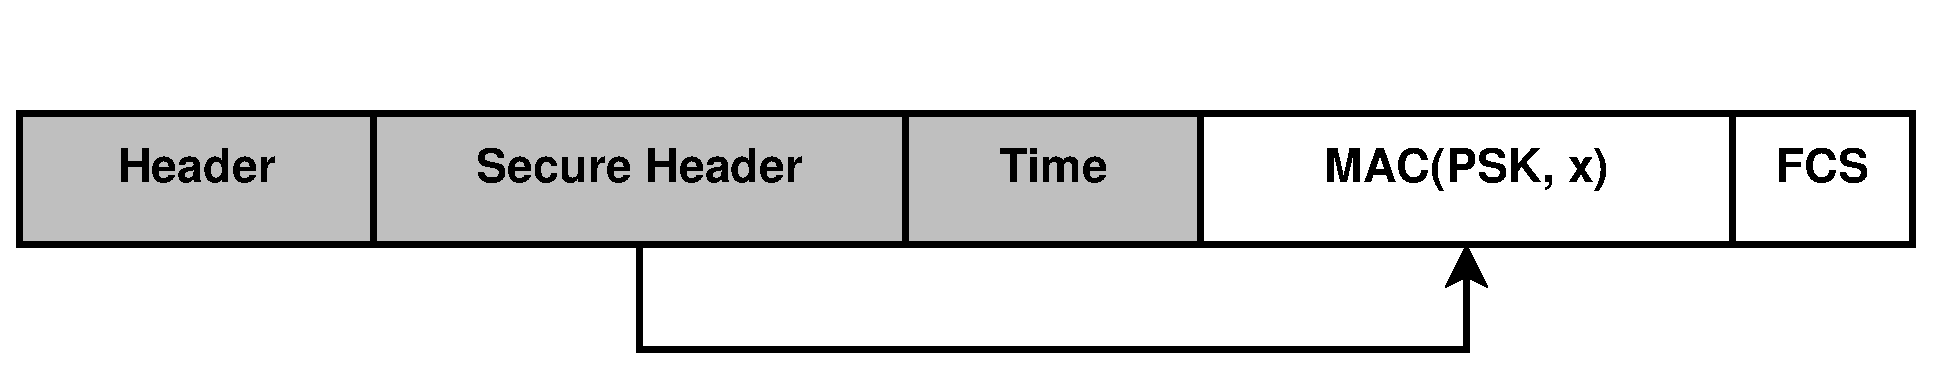
\includegraphics[width=1\textwidth]{figures/formatSyncReq.eps}
 \caption{Synchronization request frame layout}
 \label{fig:syncReqFormat}
\end{figure}
\\
\\
Every device receiving such a request checks the integrity of the message first by recalculating the \gls{mac2}. Afterwards, freshness is checked by comparing
the supplied time with it's local time. If the timing information equals the device's own local time, the device sends a unicast synchronization response
frame, containing it's local time and the actual counter value \ref{fig:syncResFormat}. The accuracy of the time comparison is deliberately reduced by defining
a window of allowed deviation. This allows a new device to join the network even it's local time and the local time of the answering device are not 
perfectly synchronized.
\begin{figure}
  \centering
    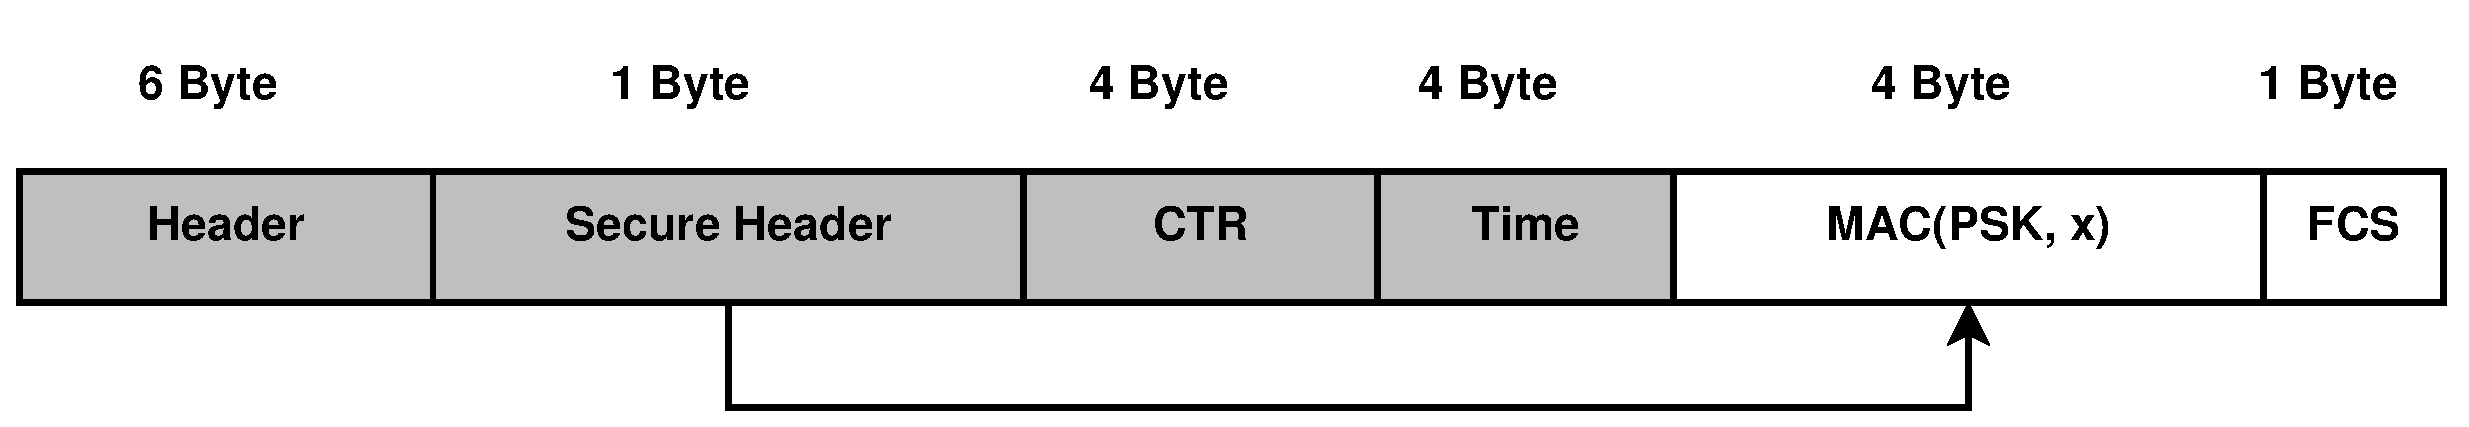
\includegraphics[width=1\textwidth]{figures/formatSyncRes.eps}
 \caption{Synchronization response frame layout}
 \label{fig:syncResFormat}
\end{figure}
If no synchronization response is received within 500ms, up to 2 retries are executed. After that, the device assumes that it is the first device in the
network and resets the global counter $Ctr_{global}$.
\\
\\
The \gls{mac2} is calculated over all frame fields except the trailing frame check fields and parts of the \textit{Header} field. 

\subsection{Discovery service}
Whenever a gateway receives a message on it's cleartext line, 2 distinct discovery broadcast messages are sent, one for each secured line. 
The frame format is shown in 
figure \ref{fig:discReqFormat}. \textit{DH-A} is the newly chosen \gls{ecdh} - parameter of the requesting device.
The \gls{psk} encrypted field contains the group address, CTR contains the incremented global counter $Ctr_{global}$.
\begin{figure}
  \centering
    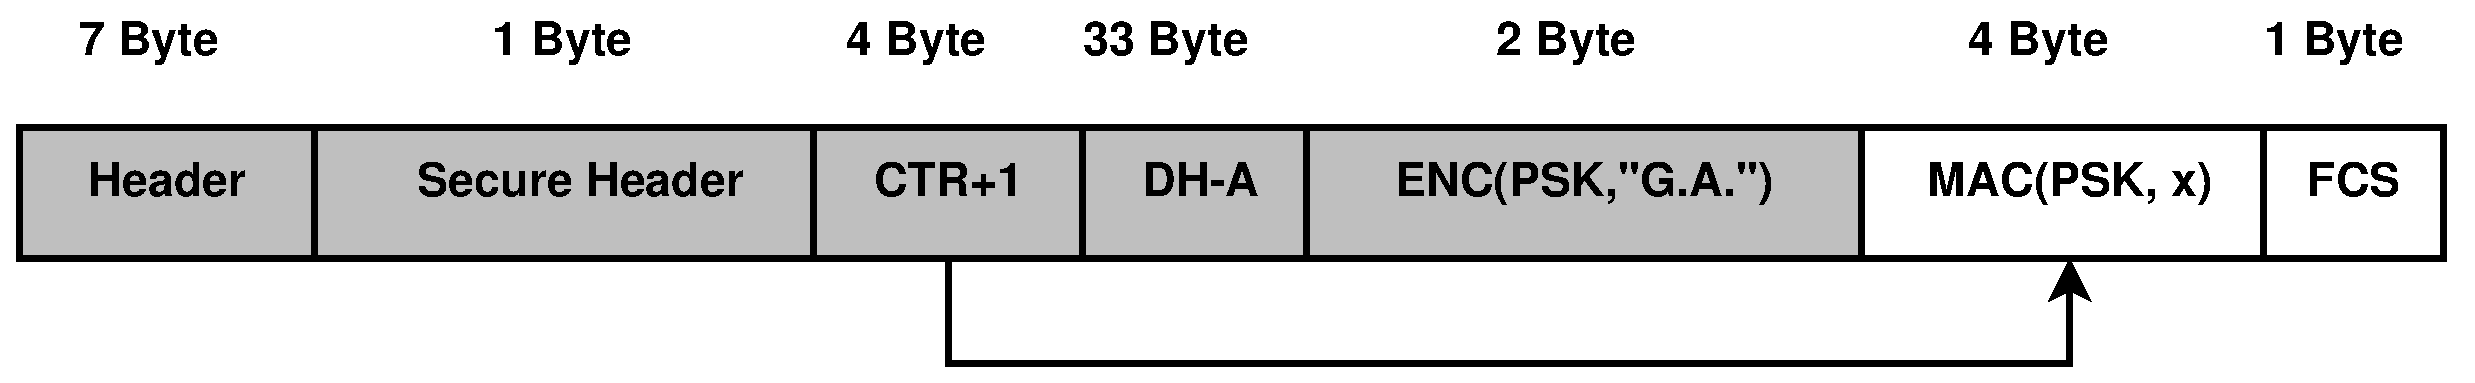
\includegraphics[width=1\textwidth]{figures/formatDiscReq.eps}
 \caption{Discovery request frame layout}
 \label{fig:discReqFormat}
\end{figure}
Every device in the network first checks the authenticity of the received frame by recalculating the \gls{mac2}. If the value differs the received one, the frame
is discarded. Otherwise, the requested group address is obtained by decrypting the corresponding field, and the device 
Every device recognizing the group address prepares a unicast response frame as shown in figure \ref{fig:discResFormat}, 
with \textit{DH-B} it's own newly chosen \gls{ecdh} parameter and the incremented global counter in the \textit{CTR} field. The wanted group address is also
sent, allowing the requester to identify the response message.
\begin{figure}
  \centering
    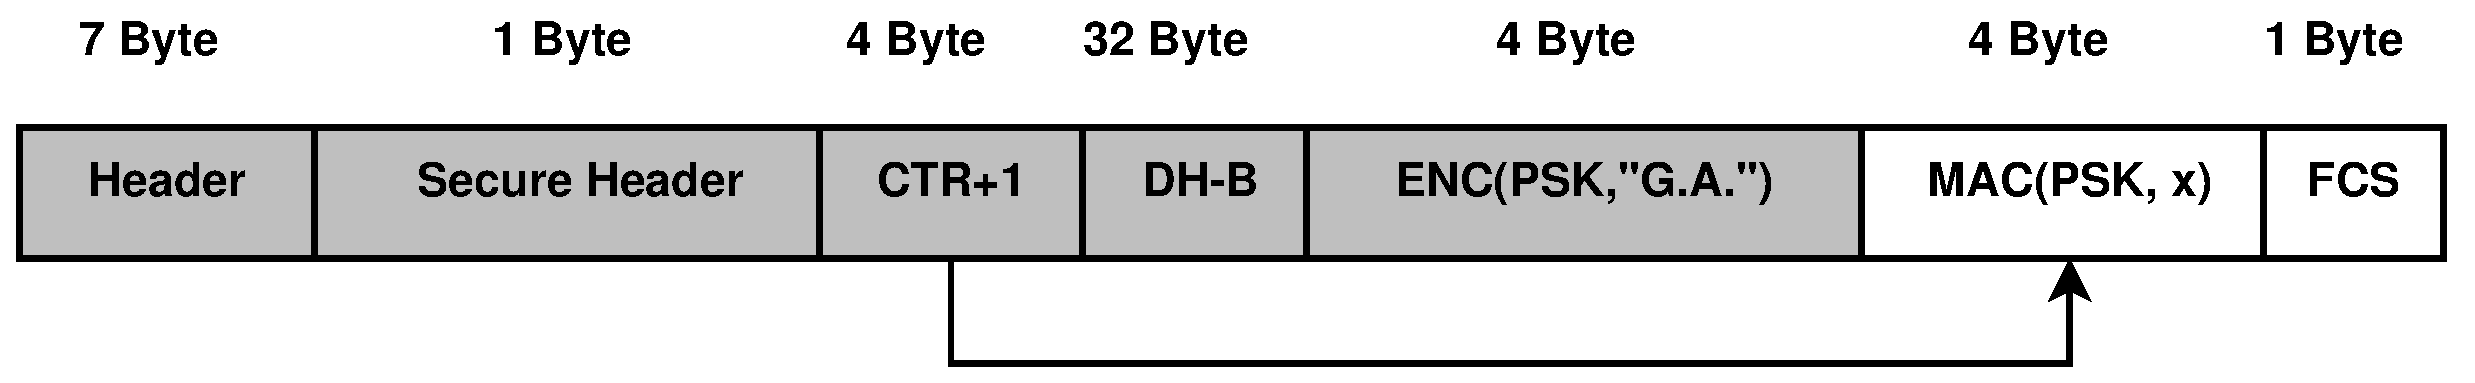
\includegraphics[width=1\textwidth]{figures/formatDiscResp.eps}
 \caption{Discovery response frame layout}
 \label{fig:discResFormat}
\end{figure}
\\
Integrity of the discovery messages is achieved by generating a \gls{mac2} over all frame fields except the frame check field and parts of the \textit{header}
field.
\\
The main logic from the discovery request receiver's point of view is shown in the state machine in \ref{fig:discRecv}

\begin{figure}
\centering
\begin{tikzpicture}[scale=0.2]
\tikzstyle{every node}+=[inner sep=4pt]
\tikzstyle{arrow}=[draw, -latex] 
\tikzset{
    pil/.style={
           ->,
           thick,
           shorten <=1pt,
           shorten >=1pt,}
}

\usetikzlibrary{automata,positioning}
\usetikzlibrary{positioning}

\node[state,initial]												at (15,0)			(rcv)		{Receive}; 
\node[state,text width=1.5cm,align=center]		at (0,-15)		(checkMAC) {Check MAC};
\node[state,text width=1.5cm,align=center]		at (-15,-30)		(discard) {Discard};
\node[state,text width=1.5cm,align=center]		at (15,-30)		(checkCtr) {Check Counter};
\node[state,text width=1.5cm,align=center]		at (0,-45)		(decrypt) {Decrypt};
\node[state,text width=1.5cm,align=center]		at (25,-45)		(sendReply) {Send Reply};

\path[pil,->] (rcv)  edge[] node[text width=1.5cm,align=center] {} (checkMAC); 
\path[pil,->] (discard)  edge[out=90,in=200] node[text width=1.5cm,align=center] {} (rcv); 
\path[pil,->] (checkMAC)  edge[] node[text width=1.5cm,align=left] {MAC invalid} (discard); 
\path[pil,->] (checkMAC)  edge[] node[text width=1.5cm,align=left] {MAC valid} (checkCtr); 
\path[pil,->] (checkCtr)  edge[] node[text width=1.5cm,align=center] {$\le Ctr_{global}$} (discard); 

\path[pil,->] (checkCtr)  edge[] node[text width=1.5cm,align=center] {$> Ctr_{global}$} (decrypt); 
\path[pil,->] (decrypt)  edge[] node[text width=1.5cm,align=center] {GA unknown} (discard); 
\path[pil,->] (decrypt)  edge[] node[text width=1.5cm,align=center] {GA known} (sendReply); 
\path[pil,->] (sendReply)  edge[out=90,in=300] node[text width=1cm,align=right] {} (rcv); 

\end{tikzpicture}
\caption{State machine for processing discovery requests}
\label{fig:discRecv}
\end{figure}

\subsection{Data service}
After receiving one or more discovery responses on one or booth secure line, the device which wants to send the \gls{knx} payload (called requester) now knows the
\glspl{ia} which are responsible for delivering messages to the wanted \gls{ga}. The requester can also derive a shared secret based on \gls{ecdh},
which is used to encrypt the origin \gls{knx} frame and inserted into the frame after the counter value. This counter $CTR-Ind$ is an individual counter, maintained
by the gateway forwarding the \gls{knx} frame received over the cleartext line - see \ref{ctrInd} for details.
\\
Authenticity is guaranteed by calculating a \gls{mac2} over all frame fields except the frame check field.
\\
\\
Figure \ref{fig:dataFormat} shows the layout of such a data frame.

\begin{figure}
  \centering
    \includegraphics[width=1\textwidth]{figures/formatData.eps}
 \caption{Data  frame layout}
 \label{fig:dataFormat}
\end{figure}

\subsection{Data Structures}

The used data structures, referenced above, are introduced in more detail below.

\subsubsection{Secure header}\label{secHdr}
Every frame sent by a security gateway contains a 8 bit header, uniquely determining the type of the frame. Implicitly, this information also determines
the exact type of authentication, encryption or authenticated encryption mode used.

\begin{center}
\begin{tabular}{ c | c | c | c}
 \label{table:secHeader}
   bytevalue & frame type & encryption & authentication \\ \hline
   0000 0000 & invalid & x & x \\
   0000 0001 & invalid & x & x \\
   0000 0010 & synchronization request & no & yes \\
   0000 0011 & synchronization response & no & yes \\
   0000 0100 & discovery request & yes & yes \\
   0000 0101 & discovery response & yes & yes \\
   0000 1000 & data service & yes & yes \\
   0000 1001 & reserved & x & x \\
   ...  & ...  & ... & ... \\
   1111 1111 & reserved & x & x \\
\end{tabular}
\end{center}
Values 0x09 - 0xFF are not used - frames containing such values should be discarded.

\subsubsection{Global counter}\label{ctrInd}
The global counter $Ctr_{global}$ is a 4 byte integer, allowing $2^{32} \approx 4,3$ billion discovery request or response messages to be sent before overflowing,
an amount assumed sufficiently high, argued as follows:
each discovery messages consists of a frame containing 53 byte, sent with 9600 \gls{bps}, resulting in about 44 milliseconds transfer duration. Therefor,
the absolute lower bound of the duration after that $Ctr_{global}$ overflows, assumed the \gls{knx} network is occupied by discovery messages only,
is about 2 years, a very conservative estimate.

\subsubsection{Individual counter}\label{ctrInd}

Every individual counter is a 4 byte integer, responsible for duplicate detection. Two distinct types of individual counters are used: $Ctr_{out}$, referenced
by an \gls{ia}, and $Ctr_{in}$, also referenced by an \gls{ia}.
The main logic is shown in figure \ref{fig:dupSM}.
\\
Whenever a new \gls{knx} frame is received on the cleartext line and the gateway knows which gateway(s) are responsible for the
contained \gls{ga}, the sending gateway determines the outgoing counter value $Ctr_{out}[\gls{ia}]$. If an outgoing counter value for
this \gls{ia} exists 
this means that the device already sent at least one data frame to a \gls{ga}, otherwise this is the first frame. In both cases,
the counter value $Ctr_{out}[\gls{ia}]$ is incremented, saved and used as value for $Ctr_{ind}$. After that, the cleartext frame is
encrypted and inserted into a new unicast data frame, one for each secure line.
\\
\\
Upon reception (the green transition in \ref{fig:dupSM}), at first the validity of the \gls{mac2} is checked - if valid, the receiver checks it's incoming
individual counter value, referenced by the \gls{ia} of the inner frame. If the received counter value $Ctr_{ind}$ is smaller than $Ctr_{in}[\gls{ia}]$,
 $Ctr_{ind}$ is saved as $(Ctr_{in}[\gls{ia}]$ and the inner frame is forwarded. The second frame, which will be handled eventually 
afterwards will bear the counter value $Ctr_{ind} = Ctr_{in}[\gls{ia}]$ and will be discarded, thus eliminating the duplicate.

\begin{figure}
 \centering
\begin{tikzpicture}[scale=0.2]
\tikzstyle{every node}+=[inner sep=2pt]
\tikzstyle{arrow}=[draw, -latex] 
\tikzset{
    pil/.style={
           ->,
           thick,
           shorten <=1pt,
           shorten >=1pt,}
}

\usetikzlibrary{automata,positioning}
\usetikzlibrary{positioning}

\node[state,initial,text width=1cm,align=center]					at (0,-10)			(rcv)		{ rcv}; 
%\node[state,text width=2cm,align=center]					at (0,-15)			(chkCtr)		{Check Counter}; 
\node[state,text width=2.2cm,align=center]					at (-15,-30)			(ctrNew)		{$Ctr_{out}[IA] = 1$}; 
\node[state,text width=2.2cm,align=center]					at (15,-30)			(ctrKnown)	{ inc $Ctr_{out}[IA]$}; 
\node[state,text width=2.0cm,align=center]					at (0,-40)			(dup)		{duplicate, encrypt, send}; 
\node[state,text width=1.5cm,align=center]					at (-15,-55)			(rcv1)		{check MAC, decrypt}; 
\node[state,text width=1.5cm,align=center]					at (15,-55)			(rcv2)		{check MAC, decrypt}; 
\node[state,text width=1.4cm,align=center]					at (0,-70)			(discard)		{Discard}; 
\node[state,text width=1.5cm,align=center]					at (0,-90)			(chk)		{Check Counter}; 
\node[state,text width=1.4cm,align=center]					at (25,-90)			(fwd)		{Forward Frame}; 


\path[pil,->] (rcv)  edge[] node[text width=2cm,align=left] {$Ctr_{out}[IA]$ unknown} (ctrNew); 
\path[pil,->] (rcv)  edge[] node[text width=2cm,align=right] {$Ctr_{out}[IA]$ known} (ctrKnown); 
\path[pil,->] (ctrNew)  edge[] node[text width=1cm,align=right] {} (dup); 
\path[pil,->] (ctrKnown)  edge[] node[text width=3cm,align=right] {} (dup); 
\path[pil,->,color=green] (dup)  edge[out=200,in=90] node[text width=1cm,align=right] {} (rcv1); 
\path[pil,->,color=green] (dup)  edge[out=-20,in=90] node[text width=1cm,align=right] {} (rcv2); 
\path[pil,->] (rcv1)  edge[] node[text width=1.5cm] {MAC invalid} (discard); 
\path[pil,->] (rcv2)  edge[]   node[text width=1.5cm] {MAC invalid} (discard); 
\path[pil,->] (rcv1)  edge[out=270,in=135]   node[text width=1cm] {MAC valid} (chk); 
\path[pil,->] (rcv2)  edge[out=270,in=45]   node[text width=1cm] {MAC valid} (chk); 
\path[pil,->] (chk)  edge[]   node[text width=1cm] {$Ctr_{ind} \le Ctr_{in}[IA]$} (discard); 
\path[pil,->] (chk)  edge[]   node[text width=1cm] {$Ctr_{ind} > Ctr_{in}[IA]$} (fwd); 
% in / out dimension problem...
%\path[pil,->] (fwd)  edge[]   node[] {} (rcv); 

\end{tikzpicture}
\caption{State machine of the duplicate detection logic}
\label{fig:dupSM}
\end{figure}


%%%%%%%%%%%%%%%%%%%%%%%%%%%%%%%%%%%%%%%%%

%%%%%%%%%%%%%%%%%%%%%%%%%%%%%%%%%%%%%%%%%
\chapter{Evaluation}
\label{ch:implementation}


\section{Master daemon}

\subsection{KNX addressing scheme}

Care must be taken that no duplicate knx addresses are used within the network. Therefore, the following addressing convention is proposed:
While it would be possible to use the same addresses on booth lines per gateway, a different scheme is used.
For the secured network, the address ranges starting at address 1.1.1 to address 1.1.15 and 1.2.1 to 1.2.15 are reserved for secure line number
1 and 2 respectively, which allows a maximum of 15 gateways. Different addresses are used mainly because it facilitates debugging. Additionally, the used
address ranges can be re-used outside the secured network by standard devices anyway.
On the unsecured lines, every gateway uses an address from the range 1.0.1 - 1.0.15. Addresses are assigned in a linearly ascending way, so gateway number 1
uses addresses 1.1.1 and 1.2.1 for secure lines 1 and 2, and 1.0.1 for its unsecured line.





%%%%%%%%%%%%%%%%%%%%%%%%%%%%%%%%%%%%%%%%%

%%%%%%%%%%%%%%%%%%%%%%%%%%%%%%%%%%%%%%%%%
\chapter{Results}
\label{ch:conclusion}
\section{Contribution}
To be able to deploy a communication system in more demanding environments, it is necessary to achieve informational security combined with mechanisms for improved availability.
For \gls{knx}, extensions for securing a network against malicious attacks exist, but these extension are not able to handle a fault concerning the communication medium, as well
as \gls{dos} attacks.
Therefore, this work proposes a way to protect against transient hardware failures, as well as active and passive adversaries. For the latter, the proposal is able to resist
restricted \gls{dos} attacks, too. This is achieved by using security gateways which are connected to each other in a redundant way. Standard \gls{knx} devices are connected 
through these gateways, which copy the client's frames into two properly secured frames and send them over both communication lines. The receiving side will check the received
frames for modification, discard one of the two copies and forward the remaining one to the destined standard \gls{knx} device.
\\
\\
It was shown that the proposed solution can withstand malicious attacks, as well as transient hardware failures of one of the secured lines. Therefore, the solution allows to connect
standard \gls{knx} devices which are spatially divided in a secure manner, bridging over areas where malicious behavior cannot be ruled out.
The proposed solution can be deployed in a 'plug-and-play' 
manner, as long as the constraints defined in Section \ref{sec:opContraints} are regarded. Thus, it is possible to add confidentiality, integrity and availability to a \gls{knx}
network just where needed, coexisting with segments with low security demands. By using more than 2 secured lines, the solution can easily be extended to use $n$ instead of 2 secure threads
and communication lines, increasing availability to an even higher level.

\section{Outlook}

The following improvements to the prototype solution are proposed: 
\begin{itemize}
 \item Using a cache for the mapping of group address to security gateways and encryption keys. A gateway receiving data from a client would send a discovery message once and
 cache the address(es) of the responsible gateway(s), together with the corresponding encryption key(s). Subsequent data transfer can be executed without the need for sending
 discovery messages first, reducing the bus load. Of course, a reasonable caching time has to be found after which a cached entry is deleted because newly connected
 clients may not be reachable within this duration.
 \item Obfuscating the size of the data service messages, which  can be achieved by adding an additional length field and corresponding padding, chosen randomly. This makes it harder
 to derive communication profiles.
 \item Attacks can be detected if frames with forged \glspl{mac2} are received, allowing to send an alert to an operator. For the used platform, this can be achieved easily by connecting
 the RaspberryPis to a restricted \gls{ip} network and sending the alarm, for example, by mail or \gls{snmp}.
 Additionally, the address of the attacking device can be added to a blacklist such that traffic coming from this address is discarded immediately.
 \end{itemize}
 
\subsubsection{Restrictions }
During development, the follow restrictions were found. Of course, the constraining assumptions made in Section \ref{sec:opContraints} are still valid. 

\begin{itemize}
  \item While \gls{eibd} can send extended frames, it does not support receiving frames with payload $\geq$ 56 byte. While this clearly violates the \gls{knx} specification, no efforts
  were made to debug this behavior.
  \item With the current \gls{eibd} \gls{api}, sending raw frames is not possible, but only application- or transport layer data units. This implies that 
  it is not possible to set the source address of a written frame. Frames delivered by a security gateway are therefore sent with the gateway's device address, instead of the 
  origin device address. To make the security gateways appear fully transparent to client devices, the \gls{api} must be extended.
 \end{itemize}


 
 

%%%%%%%%%%%%%%%%%%%%%%%%%%%%%%%%%%%%%%%%%


\appendix

%%%%%%%%%%%%%%%%%%%%%%%%%%%%%%%%%%%%%%%%%
\nocite{*}	% generate complete bibliography without corresponding \cites{}

%%%%%%%%%%%%%%%%%%%%%%%%%%%%%%%%%%%%%%%%%
\chapter{Setup of the base system}
\label{ch:basesystem}
The base system consists of raspbian pi board running the raspbian operating system(a Debian variant), the EIBD daemon, shared libraries which
are used by EIBD and the master daemon.
The operating system is based on the Debian project, with the kernel, libraries and binaries ported to the ARM platform, so it is possible to benefit from
using a full-scale operating system, e.g. by using the comfortable packet manager called
\textit{aptitude} provided by Debian. A short introduction to the most important commands is given below as they are needed.

\section{Raspbian}

To obtain a running system for deploying the secure KNX daemon, a prebuilt Debian image is used, which can be ownloaded from the raspberry homepage:

\url{http://downloads.raspberrypi.org/raspbian_latest.torrent}

The image must be unzipped and copied to a suitable memorycard. First-generation raspberries(model 'A') have SD slots, while
all later models come with micro-SD slots. To copy the basic operating system to the memorycard, the linux commandline tool 'dd' can
be used. To find the correct device to write the image to, the following command can be used: 

\begin{lstlisting}[style=BashInputStyle,label=lst:kern.log]
    # tail -f /var/log/kern.log
\end{lstlisting}

After inserting the memorycard into a cardreader, look for output like that:

\begin{lstlisting}[style=BashInputStyle]
    [1004111.533698] sdb: detected capacity change from 7909408768 to 0
    [1004114.055840] sd 6:0:0:0: [sdb] 15448064 512-byte logical blocks: ...
\end{lstlisting}

Here, the proper device to use is the device /dev/sdb.
\textbf{Pay attention to use the correct device in the following command - this device will be overwritten}:

\begin{lstlisting}[style=BashInputStyle]
    # dd if=<Path to Image> of=<Device to overwrite>
\end{lstlisting}

After the write command has finished, the memory card is ready to use. For first time setup, a display must be connected via HDMI. Powering up the raspberry
opens a ncurses configuration dialogue. First thing to do is to resize the root partition to maximum size and set a password for the administrative
account. Optionally, different options like keyboard layout can be set.
To be able to operate the raspberry without external display, it is necessary to start the \gls{ssh} server under \textit{Advanced Options} and assign a 
fixed ip to the host by editing the file \textit{/etc/network/interfaces}, as shown in example \ref{lst:staticIP}. This way it is possible to connect to the
raspberry with a \gls{ssh} client. For password less logins, create an unpriviliged user and
 a \gls{ssh} public/private key pair for that user by executing these commands on the raspberry pi:

\begin{lstlisting}[style=BashInputStyle]
    # groupadd <usergroup>
    # useradd -g <usergroup> -m <username>
    # su <username>
    # ssh-keygen
\end{lstlisting}
 
The program generates the user and the correspoding key pair and saves public and private key in the subdirectory ~/.ssh/ on the actual host. When asked for a passphrase, it is possible
to use a password-less keypair, an option that should only be used in restriced areas.
To actually use the keypair for logging into
the raspberry pi, the public key must be saved in the file \textit{~/.ssh/authorized\_keys}. Additionally, the private key must be copied to every host
from that \gls{ssh} connections to the raspberry pi want to be opened. After that, it is possible to load the private key into memory with the command \textit{ssh-add}
and to connect to the host without a password:

\begin{lstlisting}[style=BashInputStyle]
    # ssh-add // only necessary when non-empty passwort is used for keypair
    # ssh <username>@<host-ip|host-dns-name>
\end{lstlisting}

It is also advisable to update the operating system at this time by running the following commands as user root:

\begin{lstlisting}[style=BashInputStyle]
    # apt-get update
    # apt-get install
\end{lstlisting}

This will install the latest package versions of all installed packages. New software can be installed from the command line with these commands:

\begin{lstlisting}[style=BashInputStyle]
    # apt-cache search <pattern> // print a list matching packages for <pattern> 
    # apt-get install <packagename>
\end{lstlisting}

\section{EIBD}

The maintainer of EIBD only provides binary packages for the i386 architecture, so the daemon and its prerequisites must be built from source to get
suitable binaries and shared libraries for the ARM environment. Building software under GNU Linux or *nix from source always follows this scheme:

\begin{enumerate}
 \item Downloading and extracting the source code
 \item If possible, comparing the developer supplied hash code  with the hash code of the downloaded source files with
 \textit{sha256} or one of its variants to verify that no modified software has been downloaded.
 \item Optionally, apply patches to the source code(not necessary here).
 \item Set the make-options by calling \textit{./configure <options>}, overriding default compilation options by setting the corresponding command line parameters.
 \textit{./configure --help} should print a list of valid options.
 \item Compiling the source code by calling \textit{make}.
 \item Copying the generated binaries and shared libraries into their correct place by calling \textit{make install}. This last step must always be executed
 as user root because the generated files will be copied into system directories which are not writeable by unprivileged users.
\end{enumerate}
EIBD and the needed library \textit{pthsem} are available from these locations:
\\
\\
\url{https://www.auto.tuwien.ac.at/~mkoegler/pth/pthsem_2.0.8.tar.gz}\\
\url{http://sourceforge.net/projects/bcusdk/}
\\
\\
After copying the archives to the raspberry, they must be unpacked and compiled. First the pthsem shared library, which offers user mode multi
threading with semaphores, must be compiled because it is used by EIBD. 
\begin{lstlisting}[style=BashInputStyle]
    # tar -xvzf pthsem-2.0.8.tar.gz
    # cd pthsem-2.0.8
    # ./configure
    # make
    # make install // must be executed as root
\end{lstlisting}
This will, among other things, generate the shared library \textit{libpthsem.so.20} in the directory \textit{/usr/local/lib}. \textit{/usr/local}
 is by convention the destination where self compiled software should reside.
Now that pthsem is available, which is a dependence of the EIBD daemon, EIBD itself is ready for compilation:

\begin{lstlisting}[style=BashInputStyle]
    # tar -xvzf bcusdk-0.0.5.tar.gz
    # cd bcdusk-0.0.5
    # ./configure --without-pth-test --enable-onlyeibd --enable-tpuarts
    # make
    # make install // must be executed as root
\end{lstlisting}

These steps generate the binary \textit{eibd} and lots of helper programs in the directories \textit{/usr/local/bin}, and the shared object
\textit{/usr/local/lib/libeibclient.so.0} that provides the \gls{eibd} \gls{api} and therefore is needed to be linked to the master daemon. 

\section{Revision control}

The source of the master daemon is managed by GIT. GIT is a decentralized revision-control system and is available under Debian/Raspbian after installing
the package 'git'. The command \ref{lst:git} fetches the latest version and creates a directory called 'knxSec' which contains all the needed source files,
a proper makefile \ref{lst:makefile} for the project, as well as all other needed files.

\begin{lstlisting}[style=BashInputStyle,label=lst:git]
    # git clone git@github.com:hglanzer/knxSec.git
\end{lstlisting}

\section{Busware \gls{usb} couplers}

To make the KNX TP1 bus accessible, i.e. to write datagrams to and receive datagrams from the bus, \gls{usb} dongles as shown in figure \ref{fig:busware}
from the company \textit{Busware} are used. Depending on the revision, the bus couplers creates a new device which is used as \gls{url} by the \gls{eibd}.
The coupler will be accessible by \textit{/dev/ACMx}, where x is the number of the device. It may be necessary to flash the bus couplers with the correct
firmware first. The easiest way to check this is to use command \ref{lst:kern.log} and look for output similar to listing \ref{lst:device} when plugging 
the coupler into an \gls{usb} slot.

\begin{lstlisting}[style=BashInputStyle,label=lst:device]
... usb 1-1.2: new full-speed USB device number 19 using ehci_hcd
... usb 1-1.2: New USB device found, idVendor=03eb, idProduct=204b
... usb 1-1.2: New USB device strings: Mfr=1, Product=2, SerialNumber=220
... usb 1-1.2: Product: TPUART
... usb 1-1.2: Manufacturer: busware.de
... usb 1-1.2: SerialNumber: 7543034373135130C140
... cdc_acm 1-1.2:1.0: ttyACM0: USB ACM device
\end{lstlisting}

If no such line like 7 appears, the correct firmware is available as file \textit{firmware/TPUARTtransparent.hex} inside the git project. To actually flash the 
coupler, the programming button on the bottom of the device must be kept pressed while connecting it to an \gls{usb} slot. Afterwards, the commands shown
in \ref{lst:flash} must be executed.

\begin{lstlisting}[style=BashInputStyle,label=lst:flash]
    # apt-get install dfu-programmer
    # dfu-programmer atmega32u4 erase
    # dfu-programmer atmega32u4 flash TPUARTtransparent.hex
    # dfu-programmer atmega32u4 reset
\end{lstlisting}


\begin{figure}
    \centering
    \caption{Busware KNX-USB coupler}
    \label{fig:busware}
\includegraphics[scale=0.2]{figures/busware.png}
\end{figure}

\section{UDEV}

To obtain a consistent naming scheme for the busware dongles, udev rules are provided. This way it is possible to always use the same
device file for the distinct bus lines, no matter in which ordering the dongles are connected to the raspberry.

\section{Test setup}

The test environment consists of 2 raspberry pis, as shown in figure \ref{fig:secArea}. 

\chapter{Code snippets and configuration files}

\begin{lstlisting}[style=BashInputStyle,caption={Raspbian configuration for static ip address},label=lst:staticIP]
# device: eth0
  auto  eth0
  iface eth0 inet static
  address   192.168.0.2
  broadcast 192.168.0.255
  netmask   255.255.255.0
  gateway   192.168.0.1
\end{lstlisting}

\begin{lstlisting}[style=BashInputStyle,caption={Raspbian configuration for dynamic ip address},label=lst:dynamicIP]
# device: eth0
  iface eth0 inet dhcp
\end{lstlisting}

\lstinputlisting[style=BashInputStyle,caption={Makefile for the master daemon},label=lst:makefile]{../src/Makefile}

%%%%%%%%%%%%%%%%%%%%%%%%%%%%%%%%%%

\printglossary
\printbibliography

\end{document}
